% !TEX program = xelatex
% 使用 XeLaTeX 编译
\documentclass[fontsize=12pt, paper=a4, oneside, DIV=calc]{scrbook}

% 基本设置
\usepackage[UTF8]{ctex} % 中文支持
\usepackage{fontspec} % 字体设置
\usepackage{xeCJK} % 中日韩文字支持

% 设置默认字体为无衬线体(思源黑体)
% 中文/英文字体配对:正文用思源宋体(Noto Serif CJK SC)+ Noto Serif,标题用思源黑体(Noto Sans CJK SC)+ Noto Sans,等宽用 Noto Sans Mono CJK SC

\setCJKmainfont{Noto Serif CJK SC}[Scale=MatchLowercase, AutoFakeSlant = 0.15]        % 正文字体(衬线 / 宋体样式)
\setCJKsansfont{Noto Sans CJK SC}[Scale=MatchLowercase, AutoFakeSlant = 0.15] % 无衬线(适合章节标题、图例)
\setCJKmonofont{Noto Sans Mono CJK SC}[Scale=MatchLowercase] % 等宽字体(代码、表格)

% 页面布局和外观设置
\usepackage[automark,headsepline]{scrlayer-scrpage} % 页眉页脚
\clearpairofpagestyles
\ohead{\headmark} % 页眉显示章节名
\ofoot[\pagemark]{\pagemark} % 页脚显示页码

% 数学相关包
\usepackage{amsmath, amssymb, amsthm}

% 图形和颜色
\usepackage{graphicx}
\usepackage{xcolor}
\definecolor{mainblue}{RGB}{0, 90, 156}

\usepackage{booktabs}
\usepackage{longtable}
\usepackage{array}
\usepackage{calc} % 提供增强的计算功能
% 为 Pandoc 片段提供安全的宏定义,避免 Undefined control sequence
\usepackage{graphicx}
\usepackage{listings}
\usepackage{textcomp}

\providecommand{\passthrough}[1]{#1}
% 保证只有在未定义时才提供,避免覆盖模板已有定义
\providecommand{\passthrough}[1]{#1}
\providecommand{\tightlist}{\setlength{\itemsep}{0pt}\setlength{\parskip}{0pt}}
% 自动限制图片不超出行宽并保持纵横比
\makeatletter
\def\maxwidth{\ifdim\Gin@nat@width>\linewidth \linewidth \else \Gin@nat@width\fi}
\makeatother
\setkeys{Gin}{width=\maxwidth,keepaspectratio}

% 如果希望 pandoc 生成的 \pandocbounded 包裹为 figure 环境:
\providecommand{\pandocbounded}[1]{\begin{center}#1\end{center}} % 或者 \providecommand{\pandocbounded}[1]{#1}

\usepackage{enumitem}
\setlist{nosep} % 去掉列表间距
% 超链接设置
\usepackage{hyperref}
\hypersetup{
    colorlinks=true,
    linkcolor=mainblue,
    citecolor=mainblue,
    urlcolor=mainblue,
    pdftitle={昇腾310B实战——从入门到精通边缘计算与人工智能},
    pdfauthor={周贤中}
}

% 定理环境设置
\newtheoremstyle{break}
  {\topsep}{\topsep}%
  {\itshape}{}%
  {\bfseries}{}%
  {\newline}{}%
\theoremstyle{break}
\newtheorem{theorem}{定理}[chapter]
\newtheorem{lemma}[theorem]{引理}
\newtheorem{proposition}[theorem]{命题}
\newtheorem{corollary}[theorem]{推论}
\newtheorem{definition}[theorem]{定义}
\newtheorem{example}[theorem]{例子}
\newtheorem{remark}[theorem]{注记}

% 文档信息
\title{昇腾310B实战\\从入门到精通边缘计算与人工智能}
\author{周贤中}
\date{\today}

% 文档内容开始
\begin{document}

% 封面页
\maketitle

% 前言页
\frontmatter
\chapter*{前言}
书名中的 ``实战'',核心是
``在编程实践中学习''。本书作为昇腾310B芯片的入门指南,将跳出单纯的理论讲解,通过真实的AI推理部署案例,带读者直观理解昇腾310B的硬件架构特性、Atlas工具链使用逻辑与端侧AI项目开发流程
------
从模型适配、量化优化到推理服务部署,每一个知识点都配套可落地的代码示例,让读者在动手编码的过程中,真正掌握昇腾310B的实战应用能力,实现从
``了解芯片'' 到 ``能用芯片落地项目'' 的跨越。

\subsection*{本书定位与目标读者}\label{本书定位与目标读者}

本书面向以下三类读者:

\begin{itemize}
\tightlist
\item
  \textbf{高校学生 /
  科研新人}:希望通过一套系统化路径快速理解边缘AI硬件与部署流程。
\item
  \textbf{嵌入式 / IoT 工程师}:已有一定Linux / C /
  Python基础,希望把AI模型真正跑在边缘端并做性能调优。
\item
  \textbf{AI应用开发者 /
  创客}:已经能使用主流深度学习框架,希望将训练好的模型迁移到昇腾310B进行高效推理与产品化落地。
\end{itemize}

阅读预期:

\begin{itemize}
\tightlist
\item
  零基础读者可依照``快速起步路径''完成第1\textasciitilde3章+精选案例;
\item
  进阶读者可继续深入算子优化、系统整合与复杂多模型协同部署;
\item
  有项目诉求的团队可参考``方法论 +
  附录模板''直接搭建属于自己的边缘AI应用。
\end{itemize}

\subsection*{学习路径速览(建议路线)}\label{学习路径速览建议路线}

\begin{enumerate}
\def\labelenumi{\arabic{enumi}.}
\tightlist
\item
  环境 + 工具链:硬件认知 → 开发环境装配 → CANN工具初试
\item
  基础模型部署:图像分类→ 目标检测 → 语义分割 / OCR / NLP
\item
  性能优化:模型结构裁剪 → 精度-性能权衡(FP16 / INT8)→ 并行与pipeline
\item
  低级能力:自定义算子 → Profiling → ACL / GE 原理 → 内存与数据通路调优
\item
  系统构建:多进程/多模型协同 → 任务调度 → 监控与日志体系
\item
  实战案例:从需求分析 → 方案设计 → 模型适配 → 部署脚本 → 交付验收
\end{enumerate}

\subsection*{全书结构(初版规划)}\label{全书结构初版规划}

\begin{longtable}[]{@{}
  >{\raggedright\arraybackslash}p{(\linewidth - 6\tabcolsep) * \real{0.2500}}
  >{\raggedright\arraybackslash}p{(\linewidth - 6\tabcolsep) * \real{0.2500}}
  >{\raggedright\arraybackslash}p{(\linewidth - 6\tabcolsep) * \real{0.2500}}
  >{\raggedright\arraybackslash}p{(\linewidth - 6\tabcolsep) * \real{0.2500}}@{}}
\toprule\noalign{}
\begin{minipage}[b]{\linewidth}\raggedright
模块
\end{minipage} & \begin{minipage}[b]{\linewidth}\raggedright
章节标题
\end{minipage} & \begin{minipage}[b]{\linewidth}\raggedright
内容聚焦
\end{minipage} & \begin{minipage}[b]{\linewidth}\raggedright
读者收益
\end{minipage} \\
\midrule\noalign{}
\endhead
\bottomrule\noalign{}
\endlastfoot
Part 0 & 导读与准备 & 芯片特性、开发形态、学习地图 & 建立整体心智模型 \\
Part 1 & 昇腾310B硬件与环境 & 硬件结构、固件、驱动、系统配置、容器化 &
能独立搭建可复现环境 \\
Part 2 & CANN 软件栈核心 & CANN组件、ATC模型转换、OM模型结构、ACL编程 &
掌握模型从框架到OM全过程 \\
Part 3 & 边缘计算基础 & 边缘计算价值、典型架构、数据流、协同模式 &
会做架构选型与资源拆分 \\
Part 4 & 模型部署实战 & 分类/检测/NLP/多模态部署、性能测试、批处理与流式
& 会把主流任务完整迁移上板 \\
Part 5 & 性能与算子优化 &
Profiler使用、数据对齐、算子融合、自定义算子开发 &
会定位瓶颈并提升帧率/延迟 \\
Part 6 & 系统工程方法 & 多模型编排、任务调度、异常恢复、日志与监控 &
会构建工程级可维护部署系统 \\
Part 7 & 项目实战方法论 & 需求拆解、Baseline迭代、评测体系、交付模板 &
会组织团队快速交付边缘AI项目 \\
Part 8 & 典型综合案例 & 9个端侧AI实战案例(与 experiments 配套) &
迁移复用案例形成生产力 \\
Part 9 & 附录与工具 & FAQ、性能Checklist、脚手架模板、术语表 &
快速检索与复用加速迭代 \\
\end{longtable}

\subsection*{各模块核心要点概述}\label{各模块核心要点概述}

\begin{enumerate}
\def\labelenumi{\arabic{enumi}.}
\tightlist
\item
  昇腾310B硬件与环境
\end{enumerate}

\begin{itemize}
\tightlist
\item
  SoC架构(昇腾AI Core、内存层次、带宽特性)
\item
  开发板接口与外设(摄像头/存储/网络)
\item
  固件刷新 \& 系统初始化
\item
  Docker / 容器化开发与远程调试
\end{itemize}

\begin{enumerate}
\def\labelenumi{\arabic{enumi}.}
\setcounter{enumi}{1}
\tightlist
\item
  CANN 软件栈与模型转换
\end{enumerate}

\begin{itemize}
\tightlist
\item
  CANN组件:Driver / Runtime / Compiler / Toolkit
\item
  ATC模型转换参数详解(shape、输入格式、最优算子选择)
\item
  OM模型结构与可视化
\item
  ACL编程流程(初始化 → 内存 → 推理 → 释放)
\item
  常见错误(推理精度损失 / 内存不足 / 算子不支持)定位
\end{itemize}

\begin{enumerate}
\def\labelenumi{\arabic{enumi}.}
\setcounter{enumi}{2}
\tightlist
\item
  边缘计算原理
\end{enumerate}

\begin{itemize}
\tightlist
\item
  边云协同模式:云训练 + 边缘推理
\item
  数据生命周期:采集→预处理→推理→缓存→上报
\item
  典型架构模式(单板/多板/异构协同)
\item
  边缘QoS:功耗、热设计、延迟、稳定性
\end{itemize}

\begin{enumerate}
\def\labelenumi{\arabic{enumi}.}
\setcounter{enumi}{3}
\tightlist
\item
  模型部署与优化实践
\end{enumerate}

\begin{itemize}
\tightlist
\item
  图像分类(ResNet / MobileNet)
\item
  目标检测(YOLO / FasterRCNN)
\item
  OCR \& NLP(文本检测 + 轻量文本识别 / 中文BERT推理)
\item
  多模型串联(检测→裁剪→分类)Pipeline设计
\item
  精度 vs.~性能:Batch、FP16、算子融合、降采样策略
\end{itemize}

\begin{enumerate}
\def\labelenumi{\arabic{enumi}.}
\setcounter{enumi}{4}
\tightlist
\item
  低级算子与性能调优
\end{enumerate}

\begin{itemize}
\tightlist
\item
  Profiling 工具使用(时间线 / 算子耗时 / 内存峰值)
\item
  数据对齐与内存复用策略
\item
  常用自定义算子开发模板(算子描述 → 编译 → 集成)
\item
  典型瓶颈案例:数据搬运 \textgreater{} 计算、Host/Device同步等待
\end{itemize}

\begin{enumerate}
\def\labelenumi{\arabic{enumi}.}
\setcounter{enumi}{5}
\tightlist
\item
  系统集成与工程实践
\end{enumerate}

\begin{itemize}
\tightlist
\item
  任务调度(多进程、多线程、异步队列)
\item
  资源隔离与监控(显存 / Host内存 / 温度 / 带宽)
\item
  高可用设计:看门狗、超时熔断、故障降级
\item
  交付形态:容器镜像 / 一键部署脚本 / OTA升级
\end{itemize}

\begin{enumerate}
\def\labelenumi{\arabic{enumi}.}
\setcounter{enumi}{6}
\tightlist
\item
  项目实战方法论
\end{enumerate}

\begin{itemize}
\tightlist
\item
  需求澄清 \& 场景指标设定(Latency / FPS / Accuracy / Power)
\item
  Baseline快速验证:裁剪 vs.~重构 vs.~迁移
\item
  评测体系:功能、性能、稳定性、可维护性
\item
  SRE视角的上线准备 Checklist
\end{itemize}

\begin{enumerate}
\def\labelenumi{\arabic{enumi}.}
\setcounter{enumi}{7}
\tightlist
\item
  综合实战案例(与 \texttt{src/experiment} 配套) 包含 9
  大可复现案例:人脸打卡机、实时跟踪、智能电子琴、掌纹识别、数据采集仪、智能小车、智能相册、手势识别、聊天机器人。每个案例均提供:
\end{enumerate}

\begin{itemize}
\tightlist
\item
  需求说明 \& 功能结构图
\item
  模型与数据选择依据
\item
  转换 \& 部署脚本
\item
  性能测试报告(延迟 / 吞吐 / 资源占用)
\item
  可选 3D 打印结构件与装配说明
\end{itemize}

\begin{enumerate}
\def\labelenumi{\arabic{enumi}.}
\setcounter{enumi}{8}
\tightlist
\item
  附录与工具箱
\end{enumerate}

\begin{itemize}
\tightlist
\item
  常见报错速查表(ATC / ACL / Runtime)
\item
  模型转换与部署参数模板
\item
  性能调优Checklist(内存 / 数据流 / 并行 / 算子)
\item
  术语表 / 推荐资料 / 贡献指南
\end{itemize}

\subsection*{实践驱动与开源协作}\label{实践驱动与开源协作}

本书所有示例代码、脚本、案例与附录工具均开源托管于本仓库。欢迎通过 Issue
/ PR 反馈问题、提交改进、补充案例或翻译。我们鼓励: - 增补新模型 /
新任务的部署范式 - 分享自定义算子优化经验 - 提交性能测试报告(含硬件信息
+ 指标) - 翻译与文档校对

\subsection*{如何使用本书}\label{如何使用本书}

\begin{longtable}[]{@{}
  >{\raggedright\arraybackslash}p{(\linewidth - 6\tabcolsep) * \real{0.2500}}
  >{\raggedright\arraybackslash}p{(\linewidth - 6\tabcolsep) * \real{0.2500}}
  >{\raggedright\arraybackslash}p{(\linewidth - 6\tabcolsep) * \real{0.2500}}
  >{\raggedright\arraybackslash}p{(\linewidth - 6\tabcolsep) * \real{0.2500}}@{}}
\toprule\noalign{}
\begin{minipage}[b]{\linewidth}\raggedright
读者类型
\end{minipage} & \begin{minipage}[b]{\linewidth}\raggedright
推荐阅读路径
\end{minipage} & \begin{minipage}[b]{\linewidth}\raggedright
目标
\end{minipage} & \begin{minipage}[b]{\linewidth}\raggedright
补充建议
\end{minipage} \\
\midrule\noalign{}
\endhead
\bottomrule\noalign{}
\endlastfoot
零基础学生 & Part1 → Part2 → Part4(入门任务) & 能跑通首个模型 &
结合案例做改动实验 \\
嵌入式工程师 & Part1 → Part2 → Part5 → Part6 & 掌握部署与优化 &
关注资源与稳定性章节 \\
AI应用开发者 & Part2 → Part4 → Part7 → Part8 & 快速场景落地 &
记录调参与性能差异 \\
技术负责人 & Part0 → Part3 → Part6 → Part7 & 构建团队方法论 &
制定内部模板体系 \\
\end{longtable}

\subsection*{更新与版本计划}\label{更新与版本计划}

\begin{itemize}
\tightlist
\item
  v0.1(当前):结构规划 + 前3章草稿 + 2个示例案例
\item
  v0.3:补齐核心部署链路 + 性能调优初稿
\item
  v0.6:全案例上线 + 工程化章节完善
\item
  v1.0:补齐附录 + 全面审校 + PDF / LaTeX 发行
\end{itemize}

\subsection*{许可证与引用}\label{许可证与引用}

本书内容采用 Apache 2.0 许可证。引用本书内容请注明: \textgreater{}
《昇腾310B实战:从入门到精通边缘计算与人工智能》(GitHub:
zhouxzh/Ascend310)

\begin{center}\rule{0.5\linewidth}{0.5pt}\end{center}

欢迎加入共建,一起把``边缘AI实战''这件事做成!



% 目录
\tableofcontents

% 主内容开始
\mainmatter


% 第一章
\chapter{昇腾310B边缘计算基础}
\hypertarget{ux6607ux817e310bux5f00ux53d1ux677fux4ecbux7ecd}{%
\section{昇腾310B开发板介绍}\label{ux6607ux817e310bux5f00ux53d1ux677fux4ecbux7ecd}}

OrangePi
AIpro(8T)开发板是香橙派联合华为精心打造的高性能AI开发板,采用昇腾AI技术路线,搭载的昇腾310B为4核64位处理器+AI处理器,集成图形处理器,支持8TOPS
INT8的AI算力,拥有8GB/16GB LPDDR4X内存,可以外接32GB/64GB/128GB/256GB
eMMC模块,支持双4K高清输出。OrangePi
AIpro(8T)引用了相当丰富的接口,包括两个HDMI输出、GPIO接口、Type-C电源接口、支持SATA/NVMe
SSD 2280的M.2插槽、TF插槽、千兆网口、两个USB3.0、一个USB Type-C
3.0、一个Micro
USB(串口打印调试功能)、两个MIPI摄像头、一个MIPI屏等,预留电池接口,可广泛适用于AI边缘计算、深度视觉学习及视频流AI分析、视频图像分析、自然语言处理、智能小车、机械臂、人工智能、无人机、云计算、AR/VR、智能安防、智能家居等领域,覆盖
AIoT各个行业。 OrangePi
AIpro(8T)支持Ubuntu、openEuler操作系统,满足大多数AI算法原型验证、推理应用开发的需求。
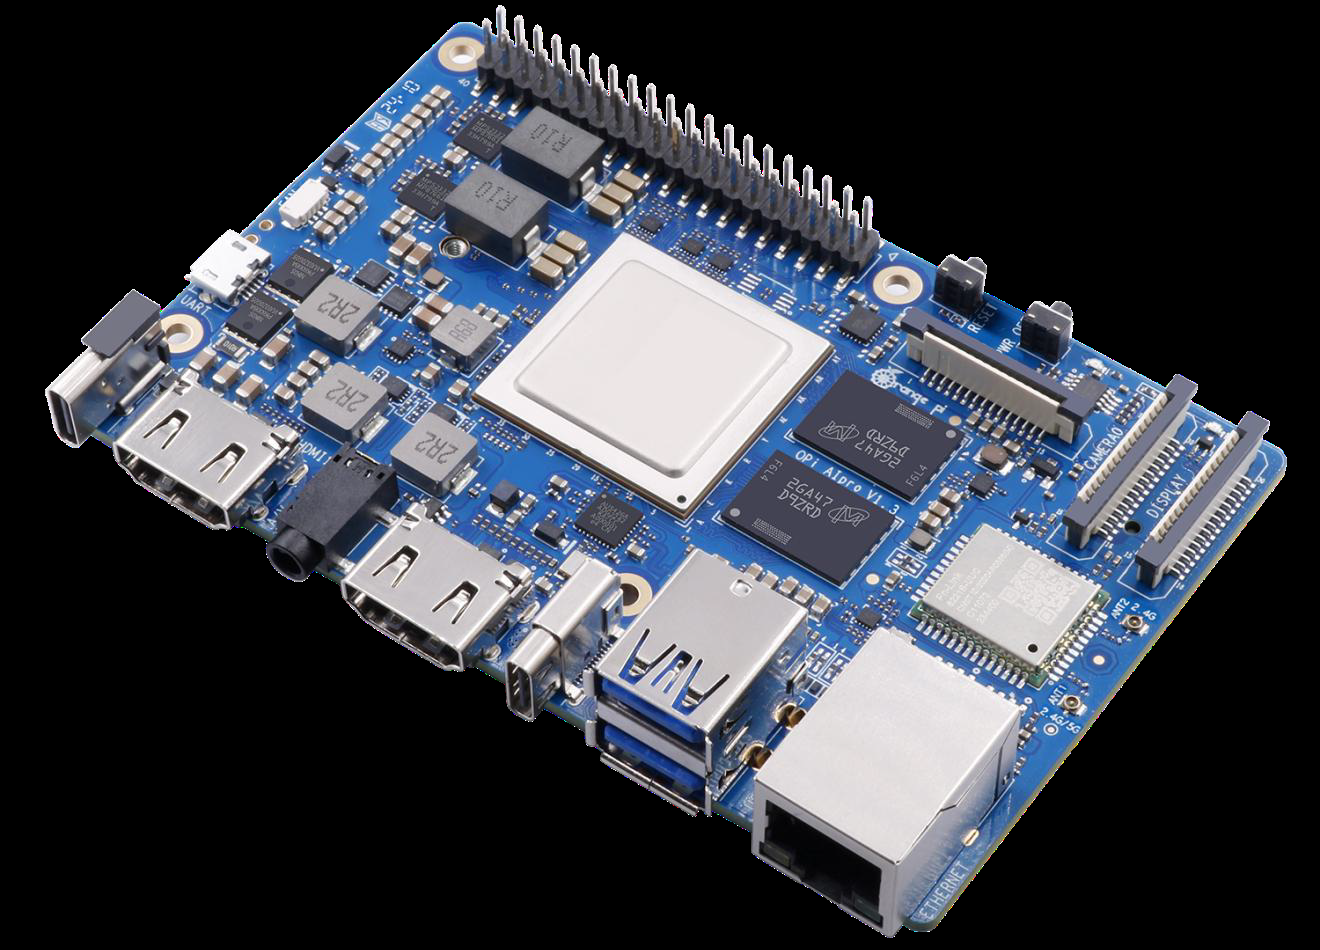
\includegraphics{img0/aipro.png}

\hypertarget{ux5f00ux53d1ux677fux8be6ux7ec6ux89c6ux56fe}{%
\subsection{开发板详细视图}\label{ux5f00ux53d1ux677fux8be6ux7ec6ux89c6ux56fe}}

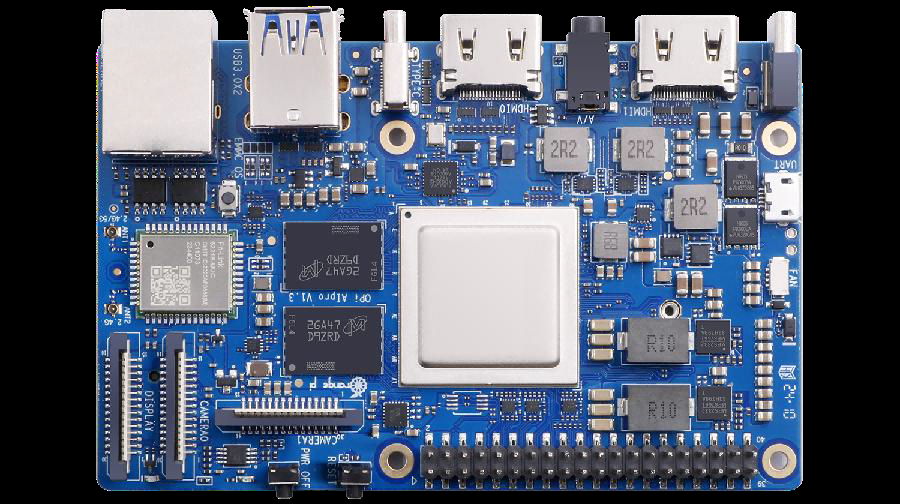
\includegraphics{img0/4.png} 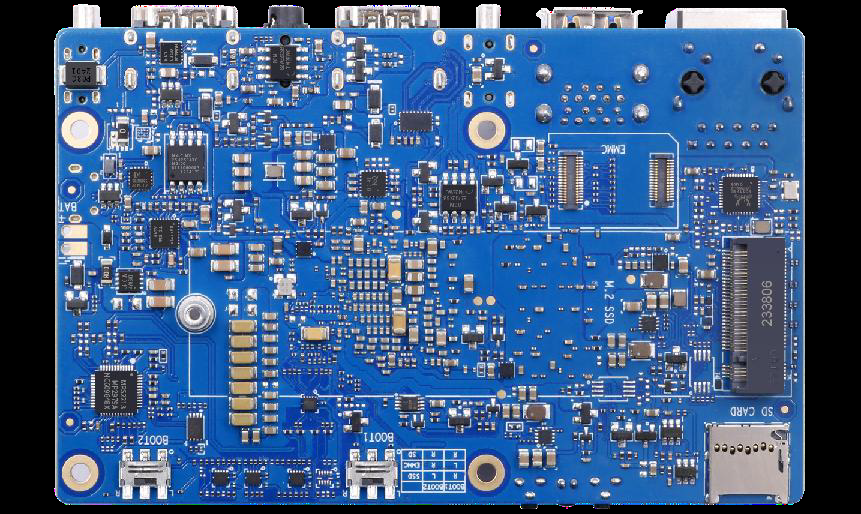
\includegraphics{img0/5.png}
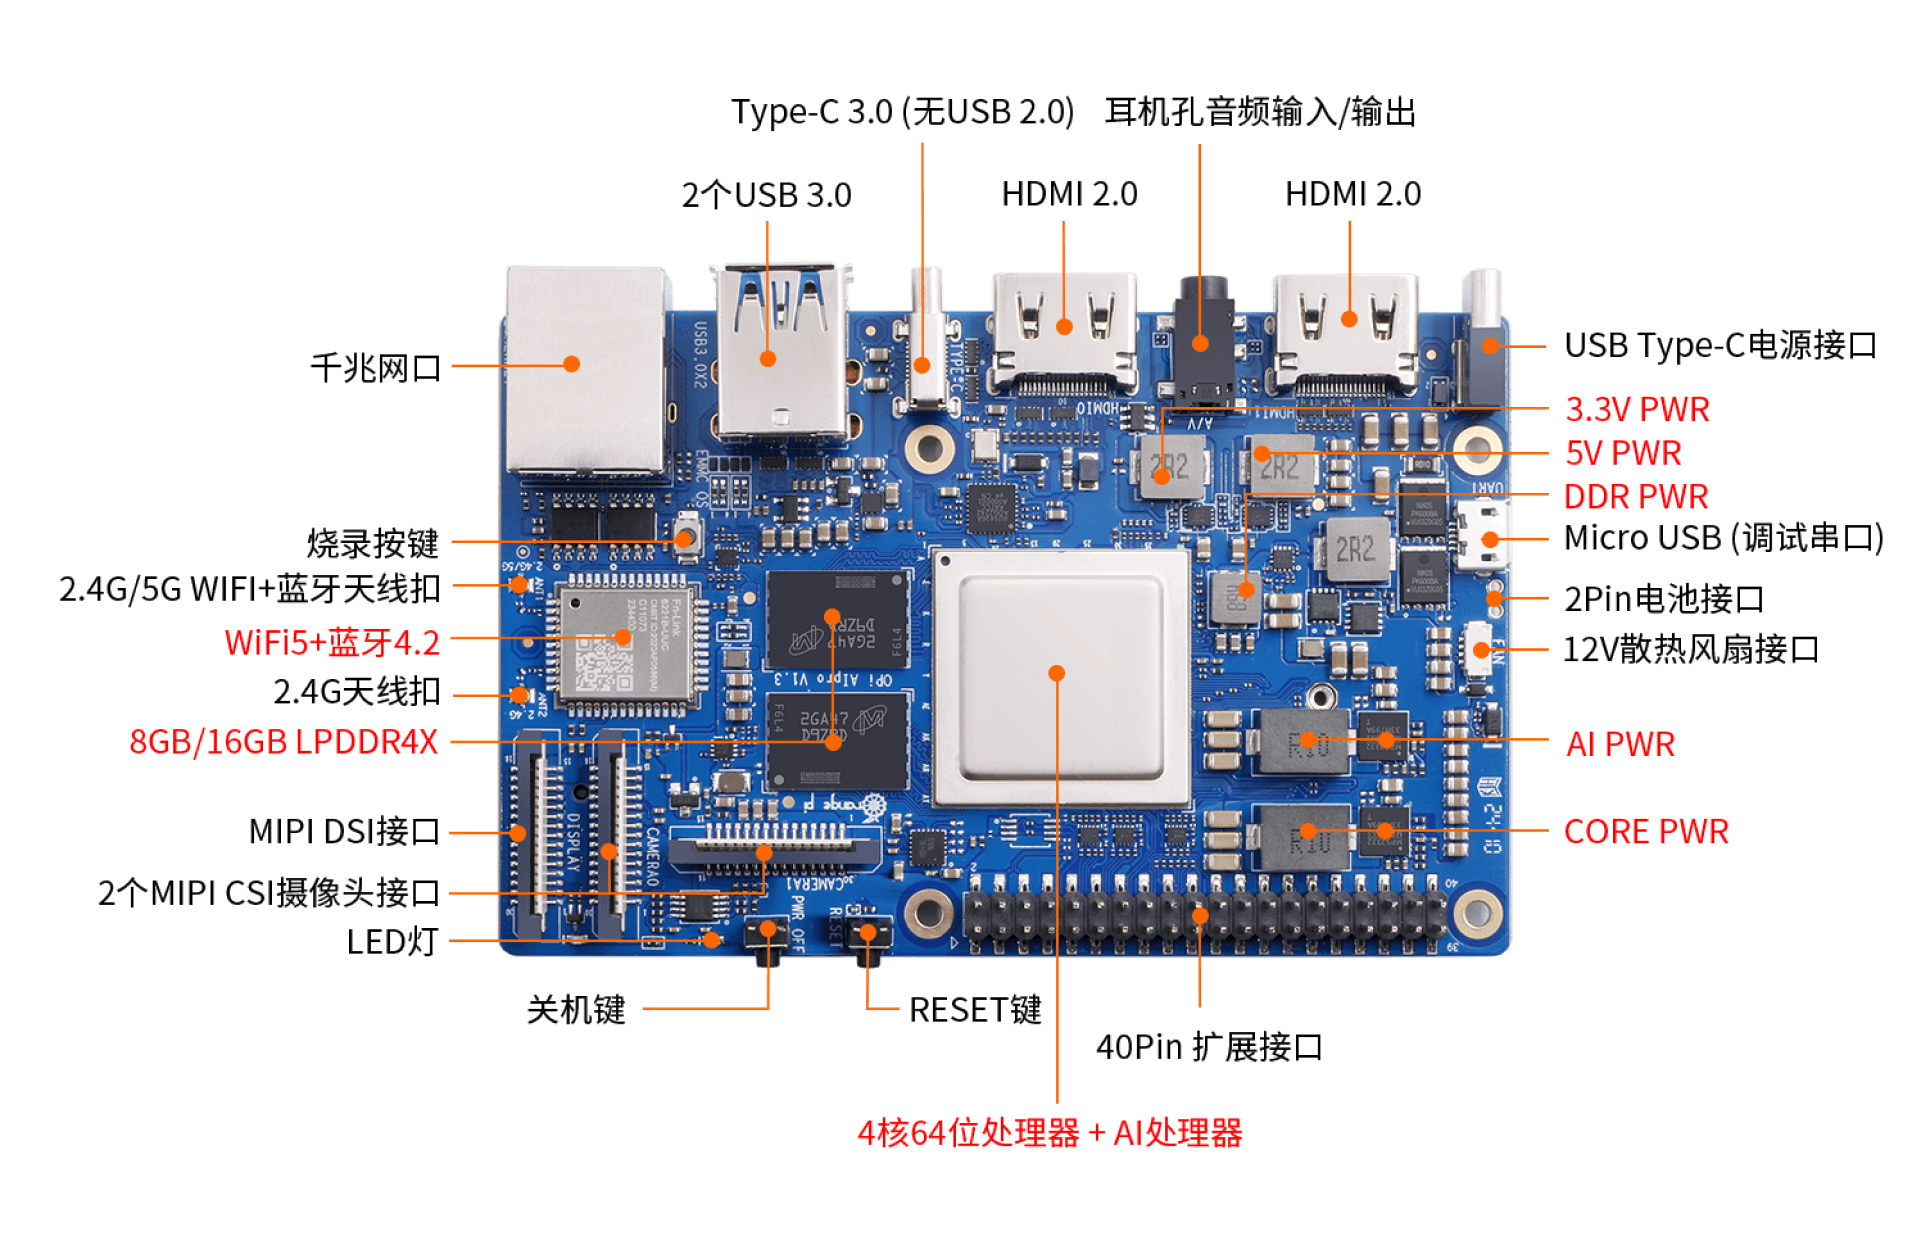
\includegraphics{img0/1.png} 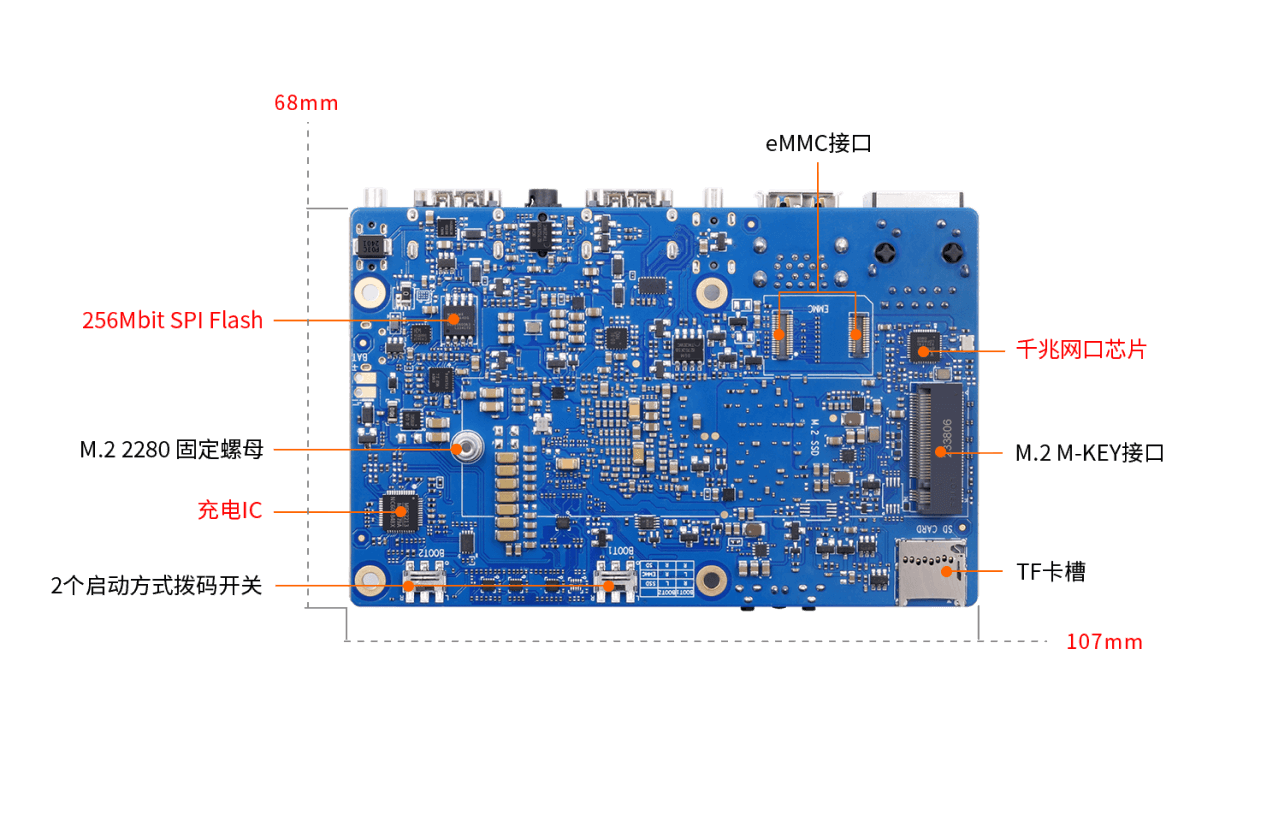
\includegraphics{img0/2.png}
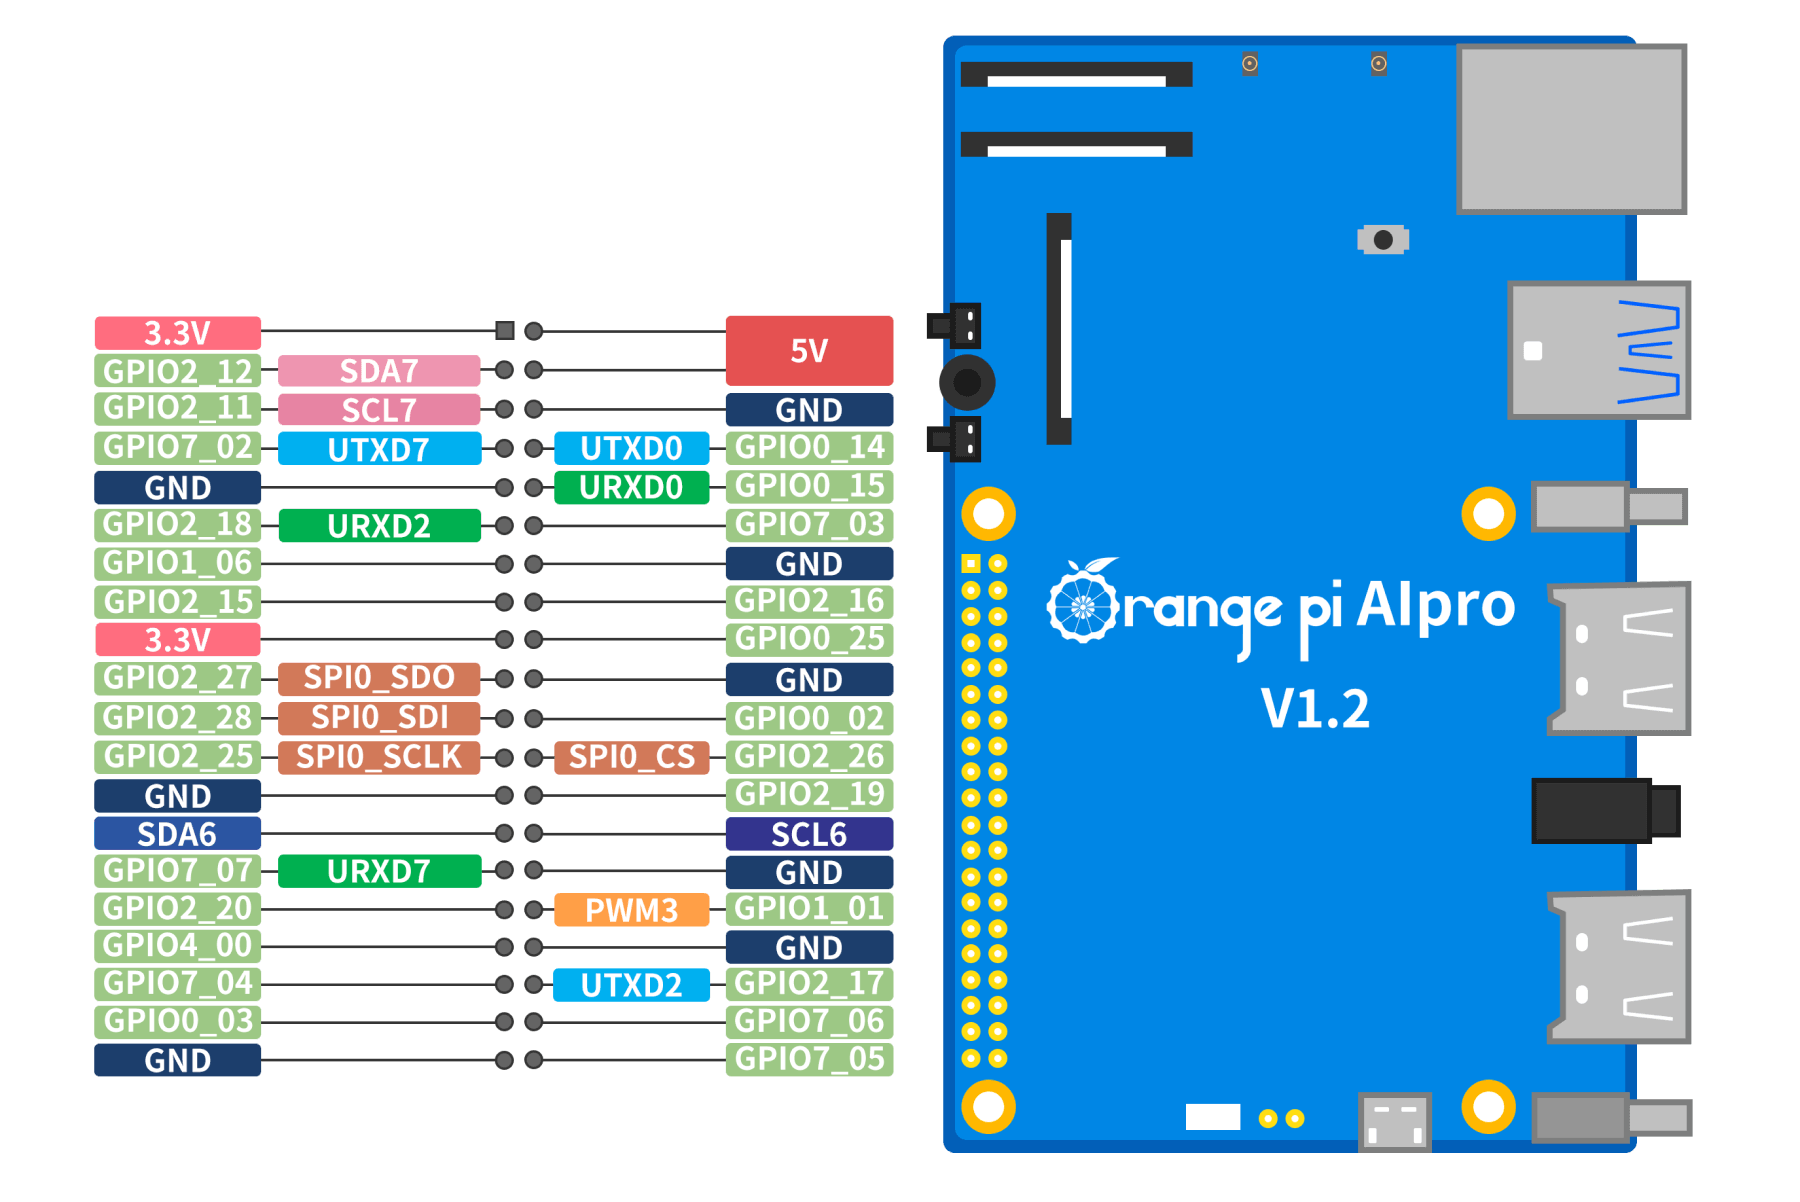
\includegraphics{img0/3.png}

\hypertarget{ux5f00ux53d1ux677fux786cux4ef6ux89c4ux683c}{%
\subsection{开发板硬件规格}\label{ux5f00ux53d1ux677fux786cux4ef6ux89c4ux683c}}

\begin{center}\rule{0.5\linewidth}{0.5pt}\end{center}

\hypertarget{ux6240ux9700ux914dux4ef6}{%
\subsection{所需配件}\label{ux6240ux9700ux914dux4ef6}}

\begin{enumerate}
\def\labelenumi{\arabic{enumi}.}
\item
  TF卡
  容量最小为32GB,速率为Class10级以上的闪迪品牌的TF卡,如下图所示。建议使用64G及以上的TF卡,以避免在开发过程中出现磁盘空间不足的问题。
  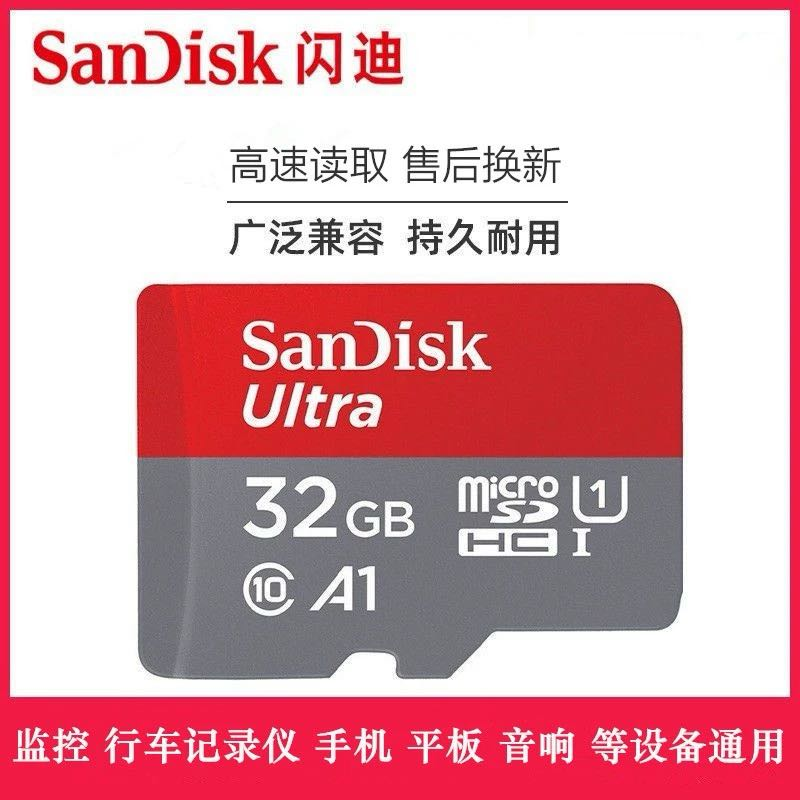
\includegraphics{img1/tf.jpg}
\item
  TF卡读卡器
  用于读写TF卡,刷写系统,建议选择速率为USB3.0以上的,减少系统刷写的等待时间。
  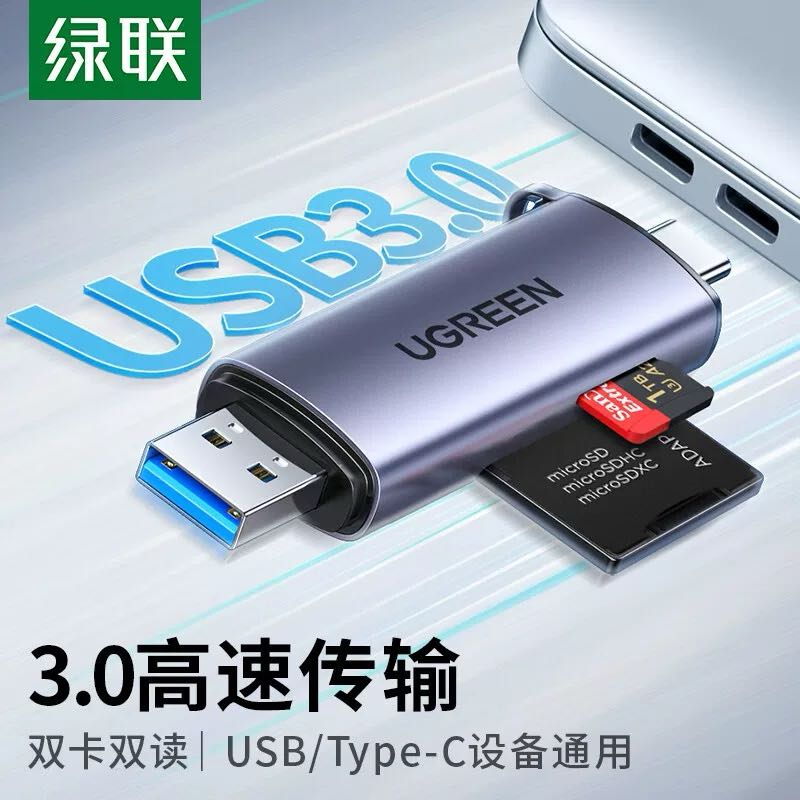
\includegraphics{img1/reader.jpg}
\item
  HDMI线或HDMI转mini-HDMI线
  主要取决于显示器的接口类型该开发板的视频输出接口为标准HDMI接口。
  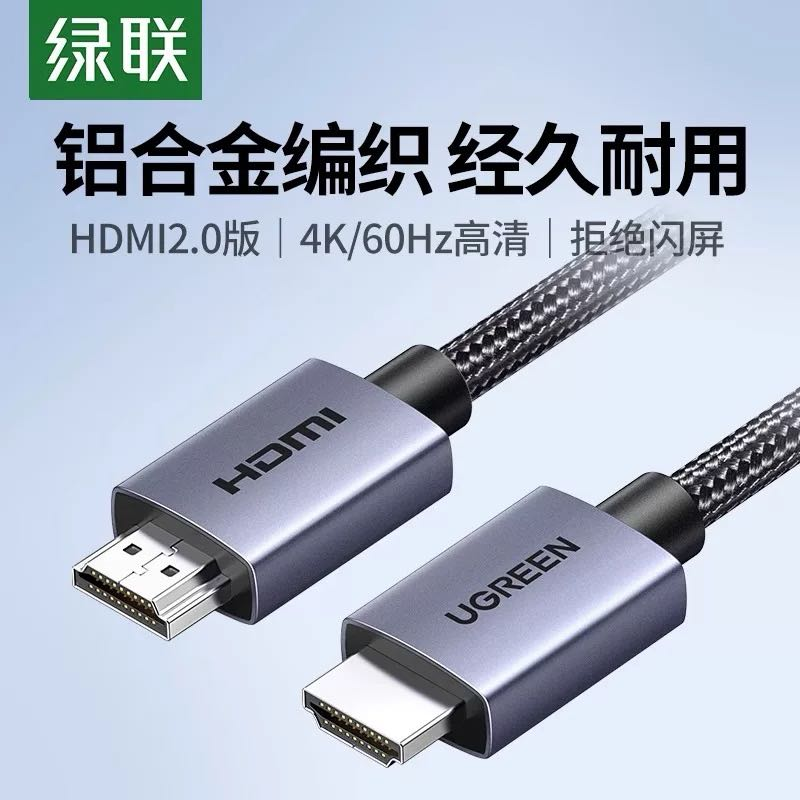
\includegraphics{img1/hdmi.jpg} 
\includegraphics{img1/minihdmi.jpg}
\item
  电源 该开发板的电源输入为PD
  20V,需要搭配支持PD协议20V挡位的65W电源适配器。
  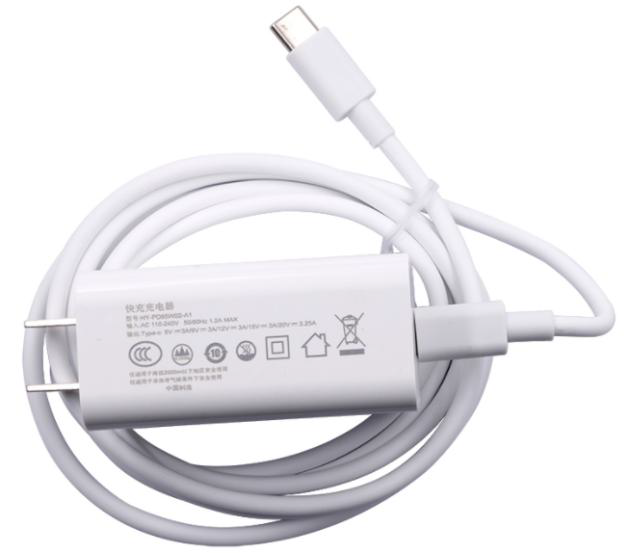
\includegraphics{img1/power.png}
\item
  USB接口的鼠标以及键盘 在无远程访问的条件下对开发板进行本地调试。
  
\includegraphics{img1/mouse.png}
\item
  金属配套外壳 用于保护开发板硬件。 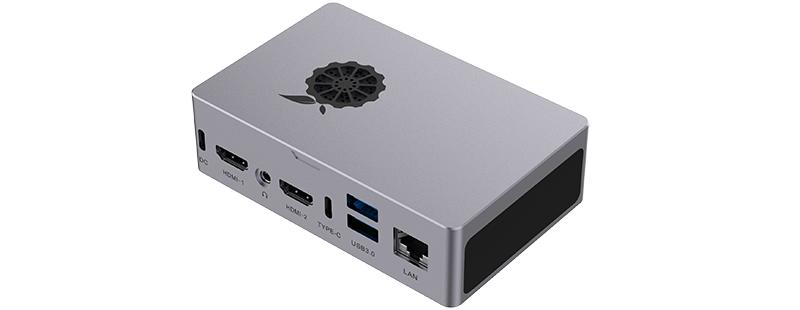
\includegraphics{img1/cover.png}
\item
  12V散热风扇以及散热鳍块
  开发板的风扇接口为2pin,输出电压为12v,支持PWM调速。由于该开发板的CPU发热较大,强烈建议安装主动扇热设备。
  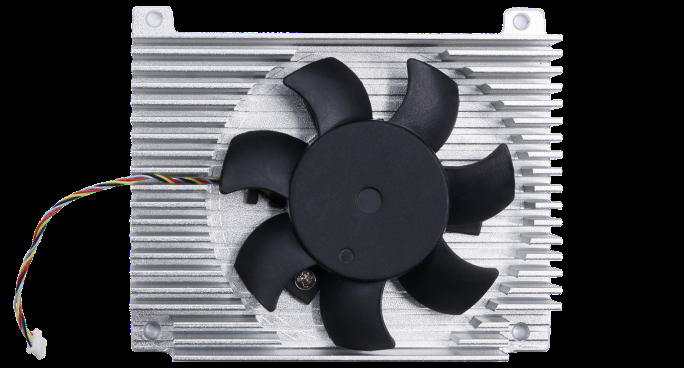
\includegraphics{img1/fan.png}
\item
  Type-C转USB 3.0转接线(可选) OrangePi
  AIPro开发板具有一个Type-C接口,协议为USB3.0(不支持USB
  2.0),可外接支持USB3.0以上协议的外置设备。
  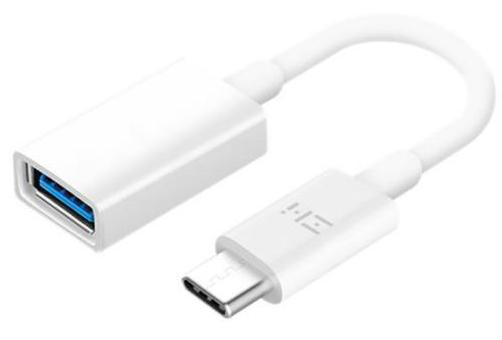
\includegraphics{img1/otg.png}
\item
  M.2接口 2280规格的PCIe Nvme SSD(可选)
  开发板的背部设计有M.2接口,可外接一个M.2的SSD作为开发板的系统盘或者存储。
  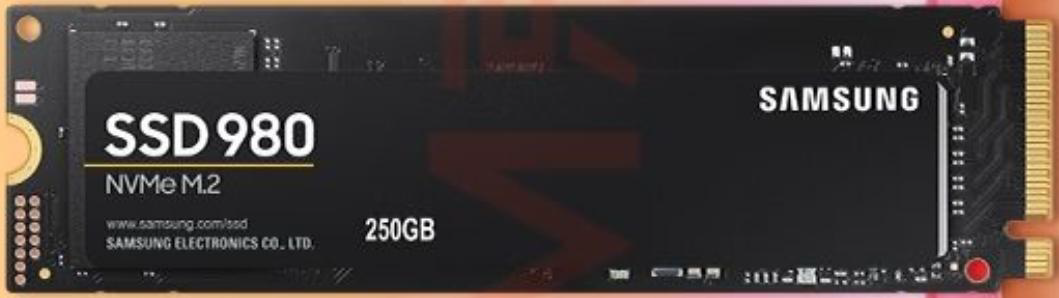
\includegraphics{img1/nvme.png}
\item
  M.2接口 2280规格的Sata Ngff SSD(可选)
  同样,开发板的M.2接口不仅支持PCIe协议,也支持Sata协议,因此也可以使用Sata协议的SSD。
  
\includegraphics{img1/ngff.png}
\item
  香橙派的eMMC模块(可选)
  eMMC(嵌入式多媒体卡)是一种集成了闪存和控制器的低成本存储解决方案,主要用于智能手机、平板电脑和低端笔记本电脑等消费电子产品。其读写速度适中(100-400MB/s),比传统机械硬盘快但不及固态硬盘(SSD),具有体积小、功耗低和易于集成的特点。开发板支持使用eMMC模块作为存储,但需要额外购置eMMC模块。
  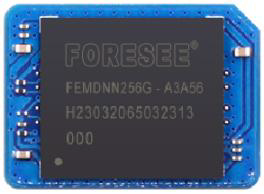
\includegraphics{img1/emmc1.png} 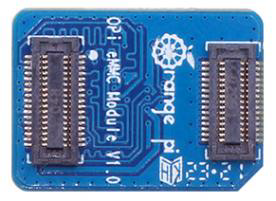
\includegraphics{img1/emmc2.png}
\item
  USB摄像头模块(可选) 可用于图像识别、视频通话等多方面用途。
  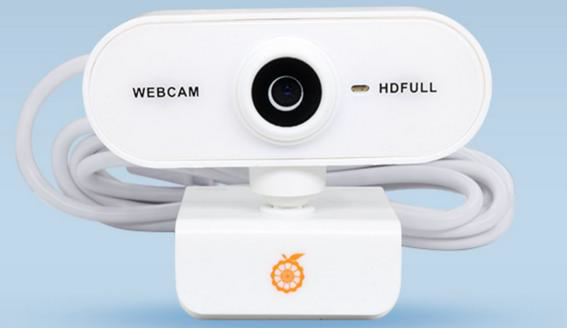
\includegraphics{img1/camera.png}
\item
  网线(可选)
  开发板自带有wifi模块可用于连接wifi,若需要更稳定的网络连接,建议使用网线连接。
  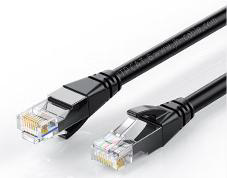
\includegraphics{img1/cable.png}
\item
  树莓派IMX219型号摄像头(MIPI-CSI)(可选)
  开发板带有两个MIPI-CSI接口,可以兼容树莓派的MIPI摄像头,无需占用USB接口。
  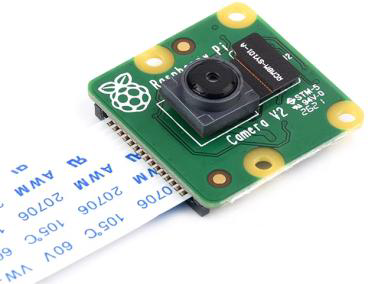
\includegraphics{img1/csi.png}
\item
  树莓派5寸MIPI LCD显示屏(可选)
  开发板带有一个MIPI-DSI显示输出接口,可以直接驱动MIPI的显示屏,而无需外接显示器。
  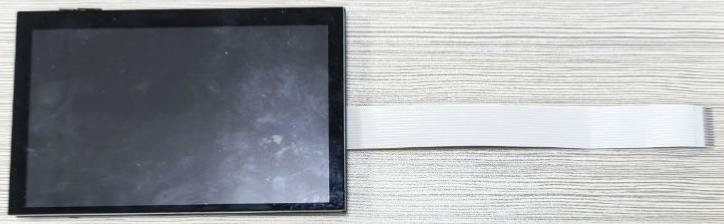
\includegraphics{img1/dsi.png}
\item
  Micro USB数据线(可选) 开发板自带了CH343P芯片,将UART转发为Micro
  USB接口,若需要使用串口对开发板进行调试,则需要使用Micro USB数据线。
  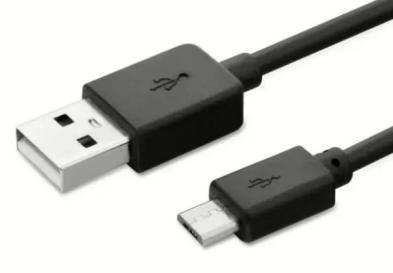
\includegraphics{img1/microusb.png}
\end{enumerate}

\hypertarget{ux4e0bux8f7dux5f00ux53d1ux677fux7684ux7cfbux7edfux955cux50cf}{%
\subsection{下载开发板的系统镜像}\label{ux4e0bux8f7dux5f00ux53d1ux677fux7684ux7cfbux7edfux955cux50cf}}

作为华为生态中重要的一员,开发板不仅支持Ubuntu系统,也支持openEuler系统,但由于开发板自身并无存储,我们在使用开发板的过程中需要使用电脑对TF卡进行系统的刷写,建议使用安装有Windows11
或 Ubuntu22.04以上版本的PC。

首先,打开香橙派官网的\href{http://www.orangepi.cn/html/hardWare/computerAndMicrocontrollers/service-and-support/Orange-Pi-AIpro.html}{技术支持界面}。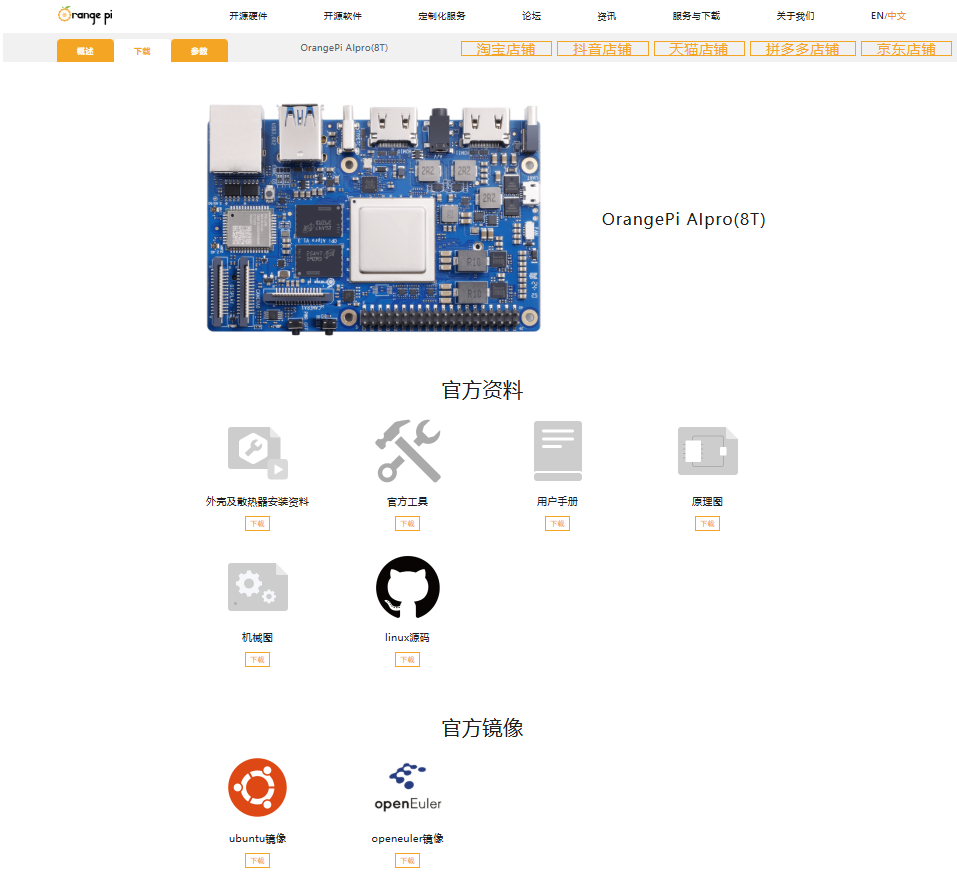
\includegraphics{img1/技术支持.png}

向下滑动网页,找到官方镜像部分,分为Ubuntu和openEuler两个部分,两个系统都是官方为我们编译完成的,且预装了部分昇腾NPU的应用环境以及软件,非常方便新手用户上手使用。

\includegraphics{img1/官方镜像.png}

\hypertarget{ubuntu}{%
\subsubsection{Ubuntu}\label{ubuntu}}

\begin{enumerate}
\def\labelenumi{\arabic{enumi}.}
\tightlist
\item
  点击下载
\includegraphics{img1/download_ubuntu.png}
\item
  复制提取码并跳转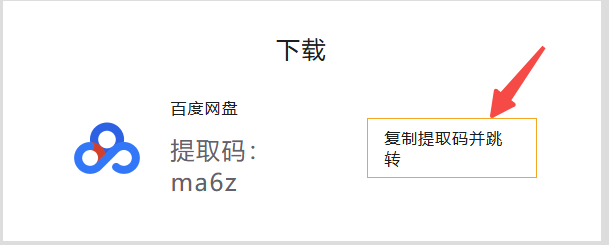
\includegraphics{img1/copyandjump.png}
\item
  打开百度网盘的链接后有一个命名为Ubuntu的文件夹,点开该文件夹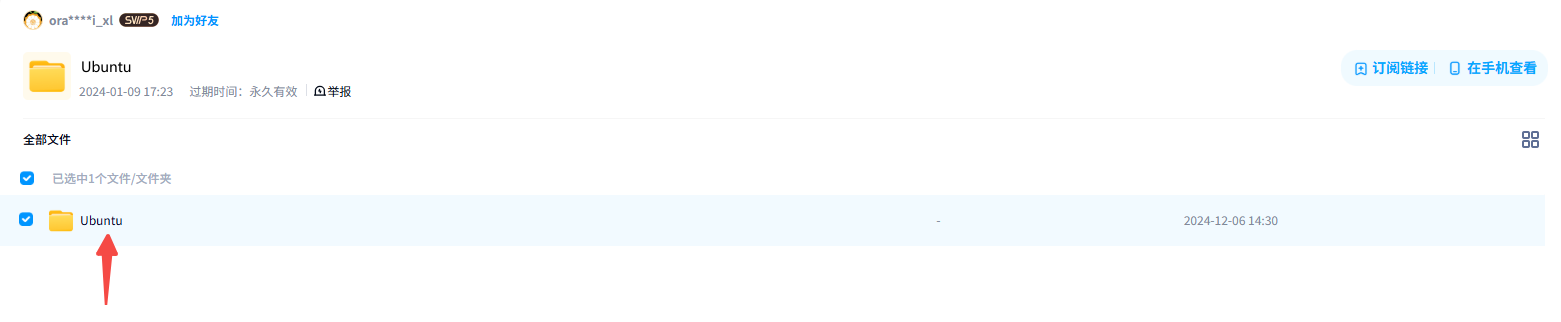
\includegraphics{img1/folder.png}
\item
  文件夹中,后缀为.xz的文件是镜像压缩包文件,.sha文件是压缩包的md5校验码文件,用于校验镜像包文件是否完整。
\item
  文件夹中的镜像有两种,一种文件名带有Desktop的,是带有GUI图形化界面的,另一种文件名带有minimal的,是不具有图形化界面的,只有命令行界面。建议新学习的用户使用带有desktop的镜像。
  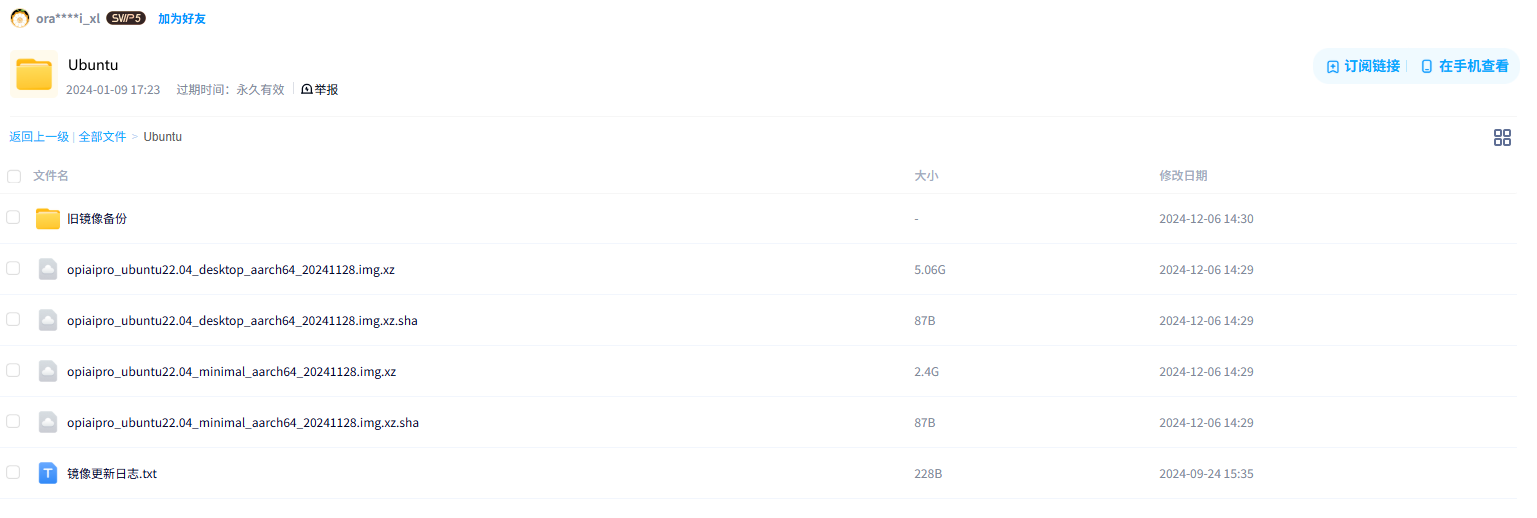
\includegraphics{img1/chooseubuntu.png}
\item
  下载后先校验压缩包是否完整,后解压压缩包
\end{enumerate}

\hypertarget{openeuler}{%
\subsubsection{openEuler}\label{openeuler}}

\begin{enumerate}
\def\labelenumi{\arabic{enumi}.}
\tightlist
\item
  点击下载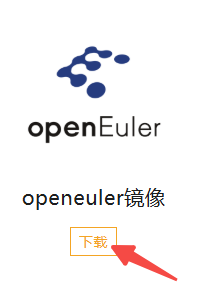
\includegraphics{img1/download_openeuler.png}
\item
  复制提取码并跳转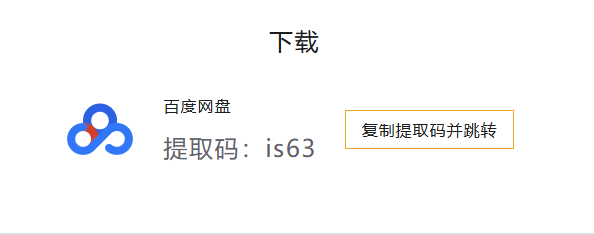
\includegraphics{img1/cpjp.png}
\item
  打开百度网盘的链接后有一个命名为OpenEuler的文件夹,点开该文件夹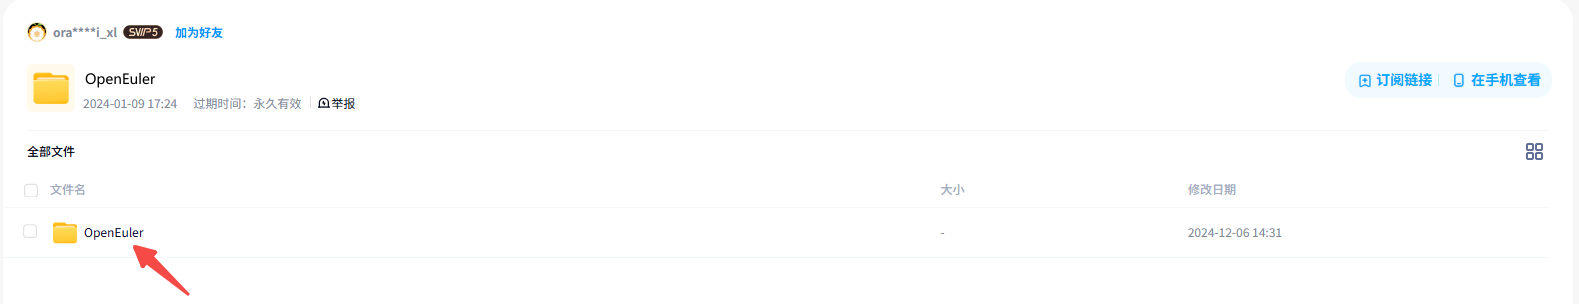
\includegraphics{img1/folderr.png}
\item
  文件夹中,后缀为.xz的文件是镜像压缩包文件,.sha文件是压缩包的md5校验码文件,用于校验镜像包文件是否完整。
\item
  文件夹中的镜像只有一种,即具有GUI图形化界面的openEuler系统。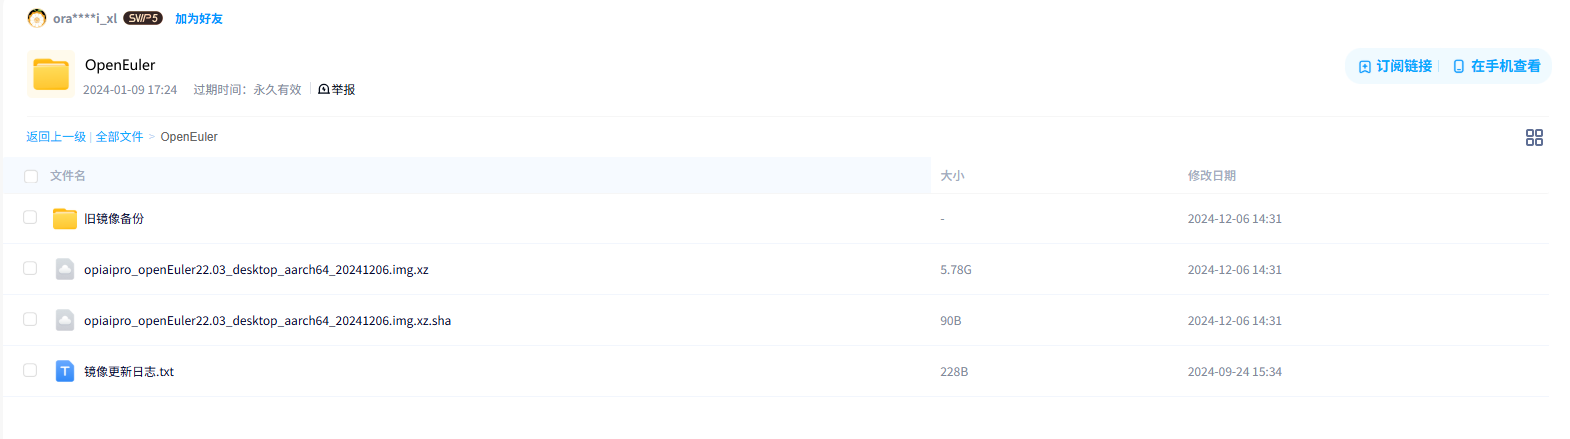
\includegraphics{img1/chooseeuler.png}
\item
  下载后先校验压缩包是否完整,后解压压缩包
\end{enumerate}

\hypertarget{ux4f7fux7528md5ux6821ux9a8cux4e0bux8f7dux7684ux6587ux4ef6}{%
\subsubsection{使用md5校验下载的文件}\label{ux4f7fux7528md5ux6821ux9a8cux4e0bux8f7dux7684ux6587ux4ef6}}

在Windows系统下,可以使用\texttt{certutil\ -hashfile\ \textless{}filename\textgreater{}\ md5};在Ubuntu系统下,可以使用\texttt{md5sum\ \textless{}filename\textgreater{}};在MacOS系统下,可以使用\texttt{md5\ \textless{}filename\textgreater{}}进行计算,此处以Windows系统为例:在文件夹按住Shift键并单击鼠标右键,选择``在终端(Powershell/命令提示符)中打开''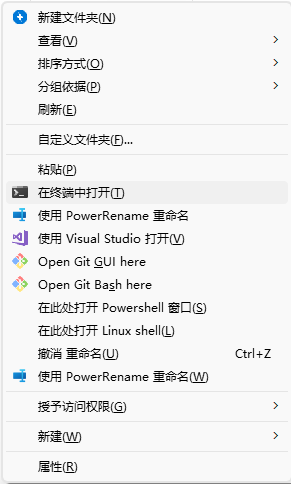
\includegraphics{img1/shell.png},然后在打开的窗口中输入\texttt{certutil\ -hashfile\ opiaipro\_ubuntu22.04\_desktop\_aarch64\_20241128.img.xz\ md5}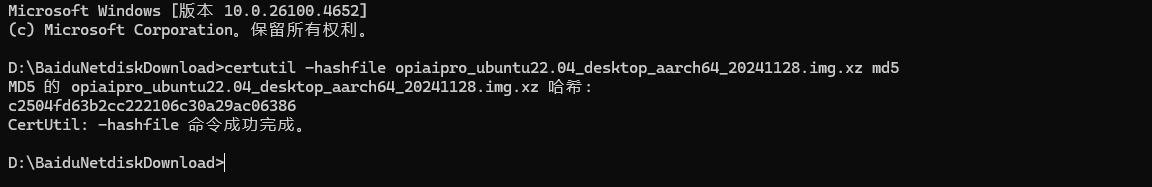
\includegraphics{img1/md5.png},将得到的md5值与\texttt{opiaipro\_ubuntu22.04\_desktop\_aarch64\_20241128.img.xz.sha}文件进行对比,若一致可进行下一步操作,否则需要重新下载。

\hypertarget{ux5237ux5199ux7cfbux7edfux5230tfux5361}{%
\subsection{刷写系统到TF卡}\label{ux5237ux5199ux7cfbux7edfux5230tfux5361}}

\hypertarget{ux4e0bux8f7dux5e76ux5b89ux88c5ux5fc5ux8981ux7684ux5de5ux5177}{%
\subsubsection{下载并安装必要的工具}\label{ux4e0bux8f7dux5e76ux5b89ux88c5ux5fc5ux8981ux7684ux5de5ux5177}}

\begin{quote}
下载链接:\href{http://www.orangepi.cn/html/hardWare/computerAndMicrocontrollers/service-and-support/Orange-Pi-AIpro.html}{官网}
\href{https://pan.baidu.com/s/1Jho73pw91r5GJD2KijY45Q?pwd=3xuz\#list/path=\%2F}{百度网盘}
1. SD Card Formatter
这个是TF卡的快速格式化工具,在每次需要刷写系统之前,都必须先对TF卡进行格式化操作,若不格式化在后续的刷写系统过程中有较大概率出错。
2. balenaEther 这个是系统镜像的刷写工具,用于刷写img镜像文件进入TF卡。
\end{quote}

\hypertarget{ux683cux5f0fux5316tfux5361}{%
\subsubsection{格式化TF卡}\label{ux683cux5f0fux5316tfux5361}}

\begin{enumerate}
\def\labelenumi{\arabic{enumi}.}
\tightlist
\item
  将TF卡插入读卡器中,并将读卡器插入电脑
\item
  打开SD Card Formatter软件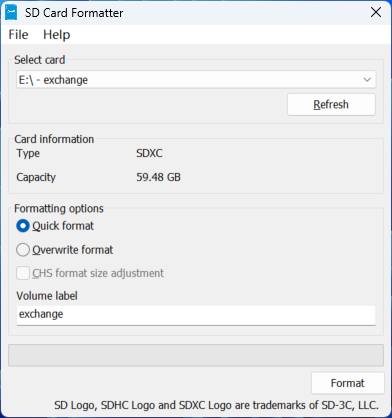
\includegraphics{img1/SDFmt.png}
\item
  点击右下角Format按键,格式化TF卡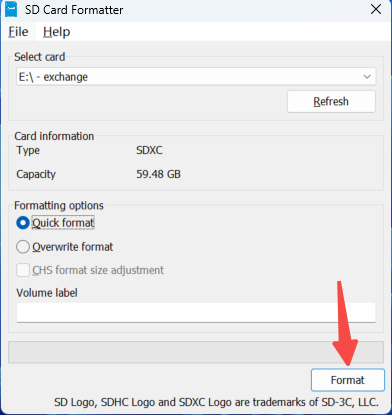
\includegraphics{img1/fmt.png}
  \textgreater{}
  警告内容是关于格式化操作会清除TF卡上原有的所有数据,此处选是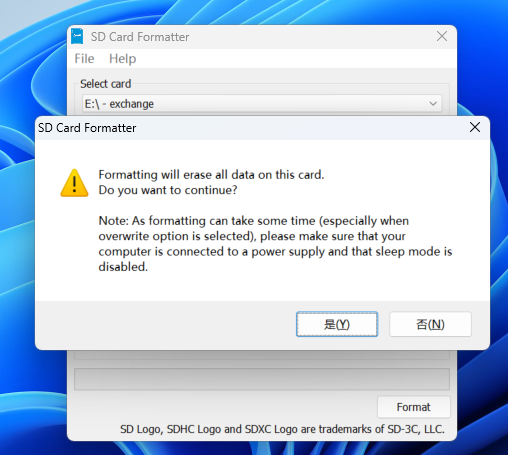
\includegraphics{img1/warning.png}
\item
  等待软件格式化完成,并点击确定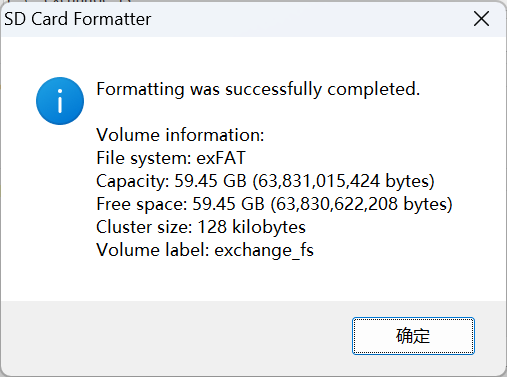
\includegraphics{img1/fmtfin.png}
\end{enumerate}

\hypertarget{ux5237ux5199ux7cfbux7edfux5230tfux5361ux4ee5ubuntuux4e3aux4f8b}{%
\subsubsection{刷写系统到TF卡(以Ubuntu为例)}\label{ux5237ux5199ux7cfbux7edfux5230tfux5361ux4ee5ubuntuux4e3aux4f8b}}

\begin{quote}
此处以Ubuntu为例 1.
打开balenaEther,选择``从文件烧录''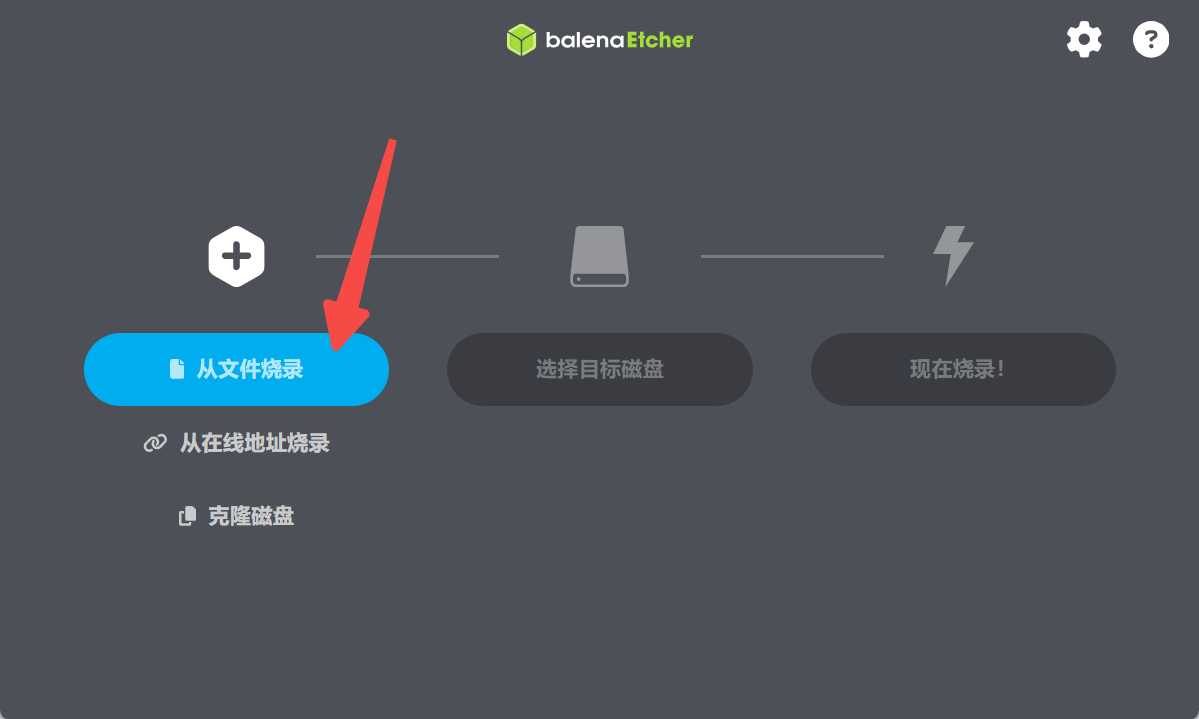
\includegraphics{img1/ether1.png} 2.
选择好要烧录的镜像文件(\textbf{.img}格式),再选择目标磁盘为TF卡对应的位置,如图中名称为``SDXC
Card''的位置,选中并选择``选定1''。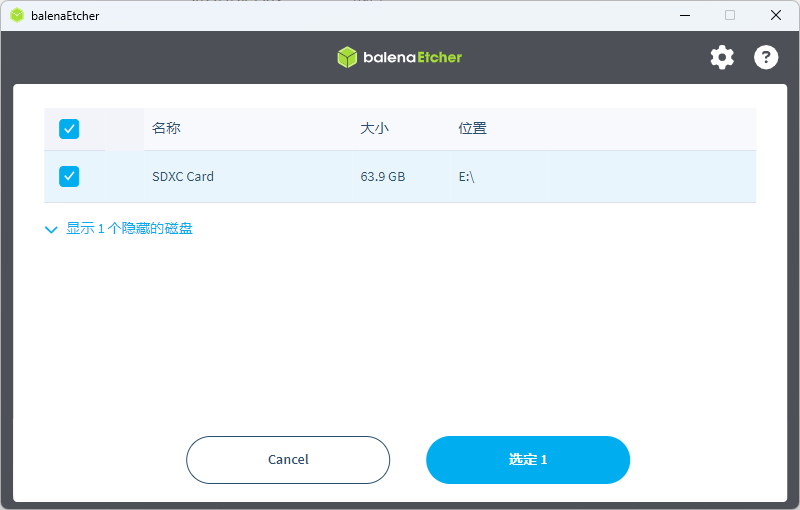
\includegraphics{img1/chooseether.png}
3. 点击``现在烧录!'',耐心等待烧录完成。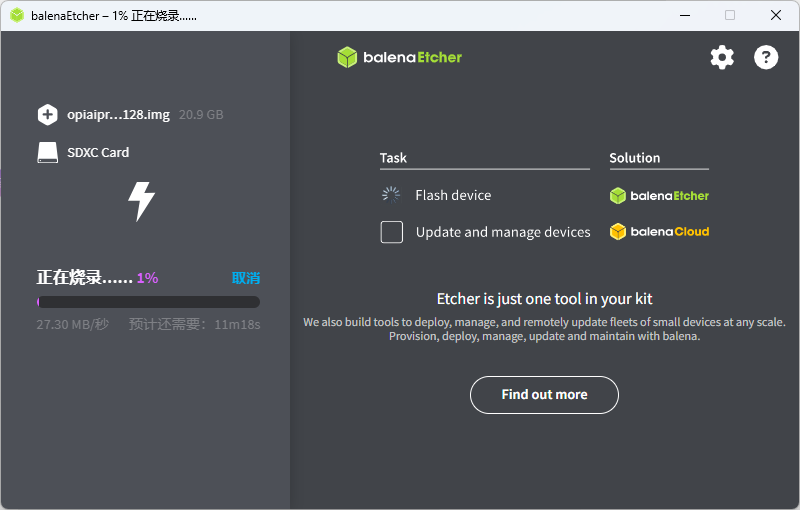
\includegraphics{img1/dd.png}
4. 烧录完成后进入校验过程,也请耐心等待。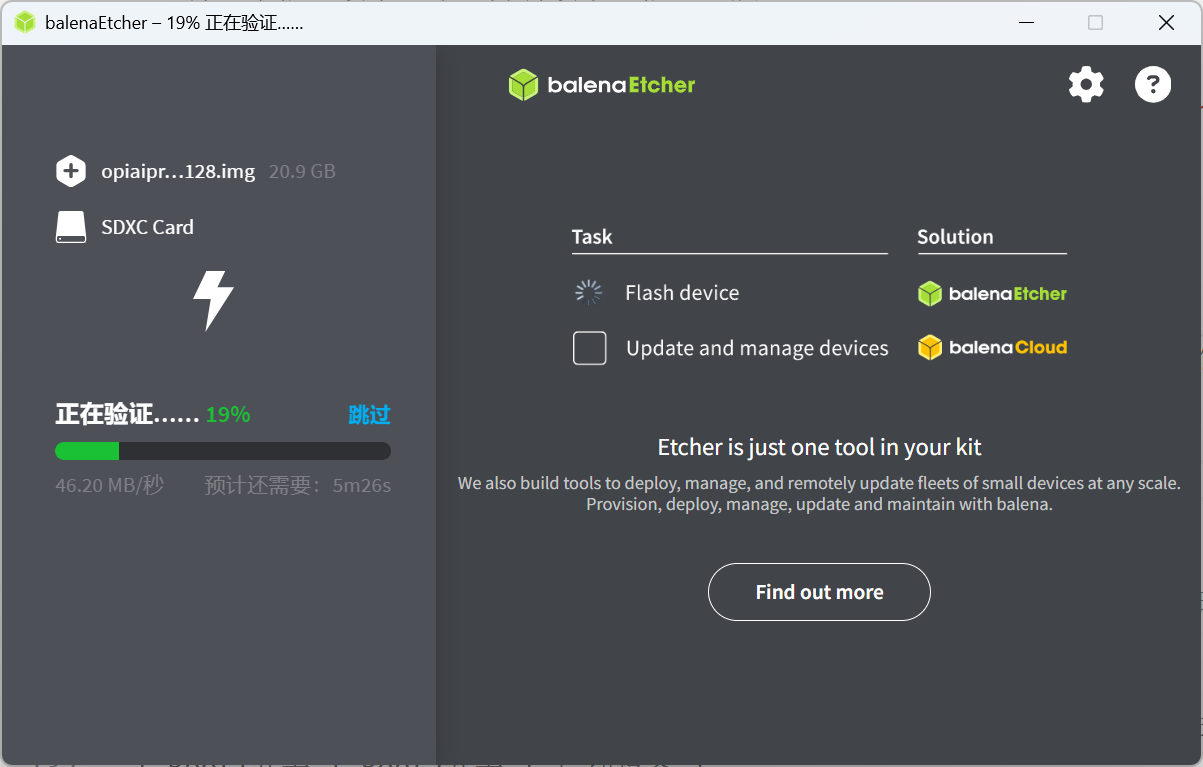
\includegraphics{img1/val.png}
5.
烧录完成后即可关闭程序,并安全弹出TF卡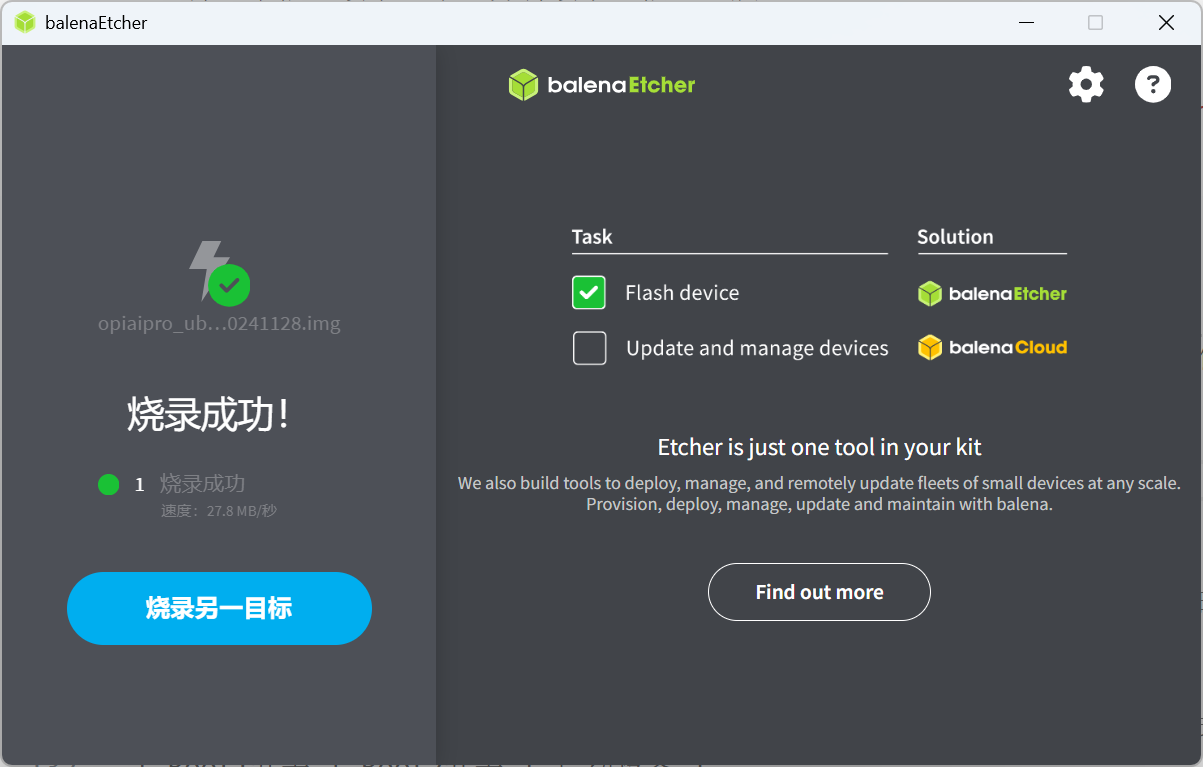
\includegraphics{img1/finish.png}
\end{quote}

\hypertarget{ux5237ux5199ux7cfbux7edfux5230emmc}{%
\subsubsection{刷写系统到eMMC}\label{ux5237ux5199ux7cfbux7edfux5230emmc}}

由于板上并不自带有eMMC模块,若要想使用需要额外购买香橙派的eMMC模块,此处暂时不列入参考,若需使用,请查阅香橙派的用户手册。

\hypertarget{ux5237ux5199ux7cfbux7edfux5230ssd}{%
\subsubsection{刷写系统到SSD}\label{ux5237ux5199ux7cfbux7edfux5230ssd}}

开发板带有M.2接口,可以使用SSD作为启动设备。但SSD需要自行准备,且根据香橙派

\hypertarget{ux8c03ux6574ux8bbeux5907ux542fux52a8ux65b9ux5f0fux7684ux62e8ux7801ux5f00ux5173}{%
\subsubsection{调整设备启动方式的拨码开关}\label{ux8c03ux6574ux8bbeux5907ux542fux52a8ux65b9ux5f0fux7684ux62e8ux7801ux5f00ux5173}}

开发板支持多种启动方式,包括TF卡、eMMC以及M.2
SSD,当这些存储设备都同时存在时,需要让开发板选定一个存储设备作为启动来源。
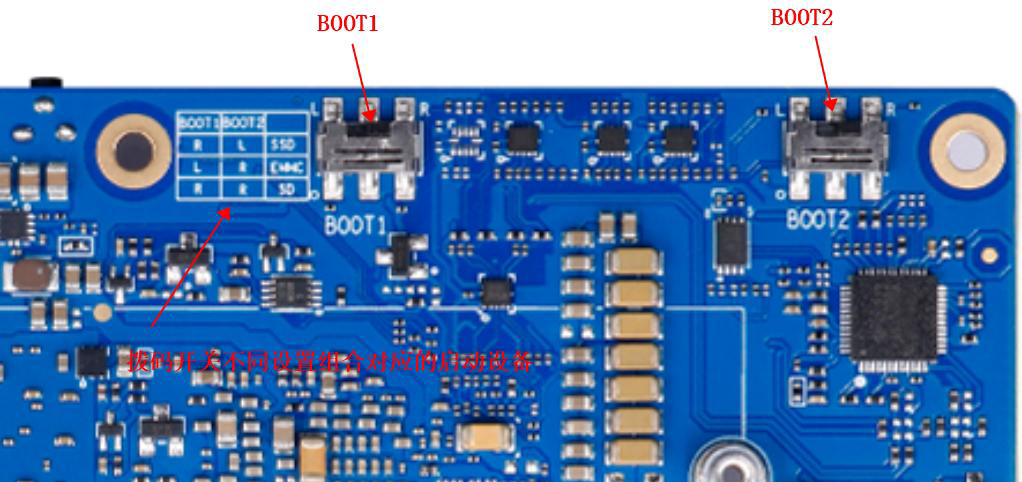
\includegraphics{img1/bootswitch.png}
两个开关都有左、右两种状态,因此共有4种状态,但是目前开发板仅使用3种模式,对应的参数表如下:
\textbar{} Boot1开关 \textbar{} Boot2开关 \textbar{} 启动设备 \textbar{}
\textbar{} :------: \textbar{} :------: \textbar{} :------: \textbar{}
\textbar{} 左 \textbar{} 左 \textbar{} 未使用 \textbar{} \textbar{} 右
\textbar{} 右 \textbar{} TF卡 \textbar{} \textbar{} 左 \textbar{} 右
\textbar{} eMMC \textbar{} \textbar{} 右 \textbar{} 左 \textbar{} M.2
SSD (Nvme或Ngff)\textbar{}
切换拨码开关后,必须要将开发板完全断电再重新上电才能使新的启动配置生效,使用RESET按键重启则不会使新的启动配置生效。

\hypertarget{ux542fux52a8ux5f00ux53d1ux677fubuntu}{%
\subsection{启动开发板(Ubuntu)}\label{ux542fux52a8ux5f00ux53d1ux677fubuntu}}

\begin{itemize}
\tightlist
\item
  图形化界面
\end{itemize}

\begin{enumerate}
\def\labelenumi{\arabic{enumi}.}
\tightlist
\item
  将系统刷写完成的TF卡从读卡器中取出,插入开发板的TF卡插槽中,并确保两个启动开关的位置均在右边,接入HDMI数据线到靠近USB3.0接口的HDMI0接口,然后将Type-C电源线插入开发板最边缘的TYPE-C供电口,等待风扇的声音变小以及屏幕出现系统登录界面。
  
\includegraphics{img1/beforelogin.png}
\item
  进入登录界面后,将键盘接入开发板的USB接口中,默认的登录用户名是\texttt{HwHiAiUser},输入该账户的密码\texttt{Mind@123},登录进入系统。
  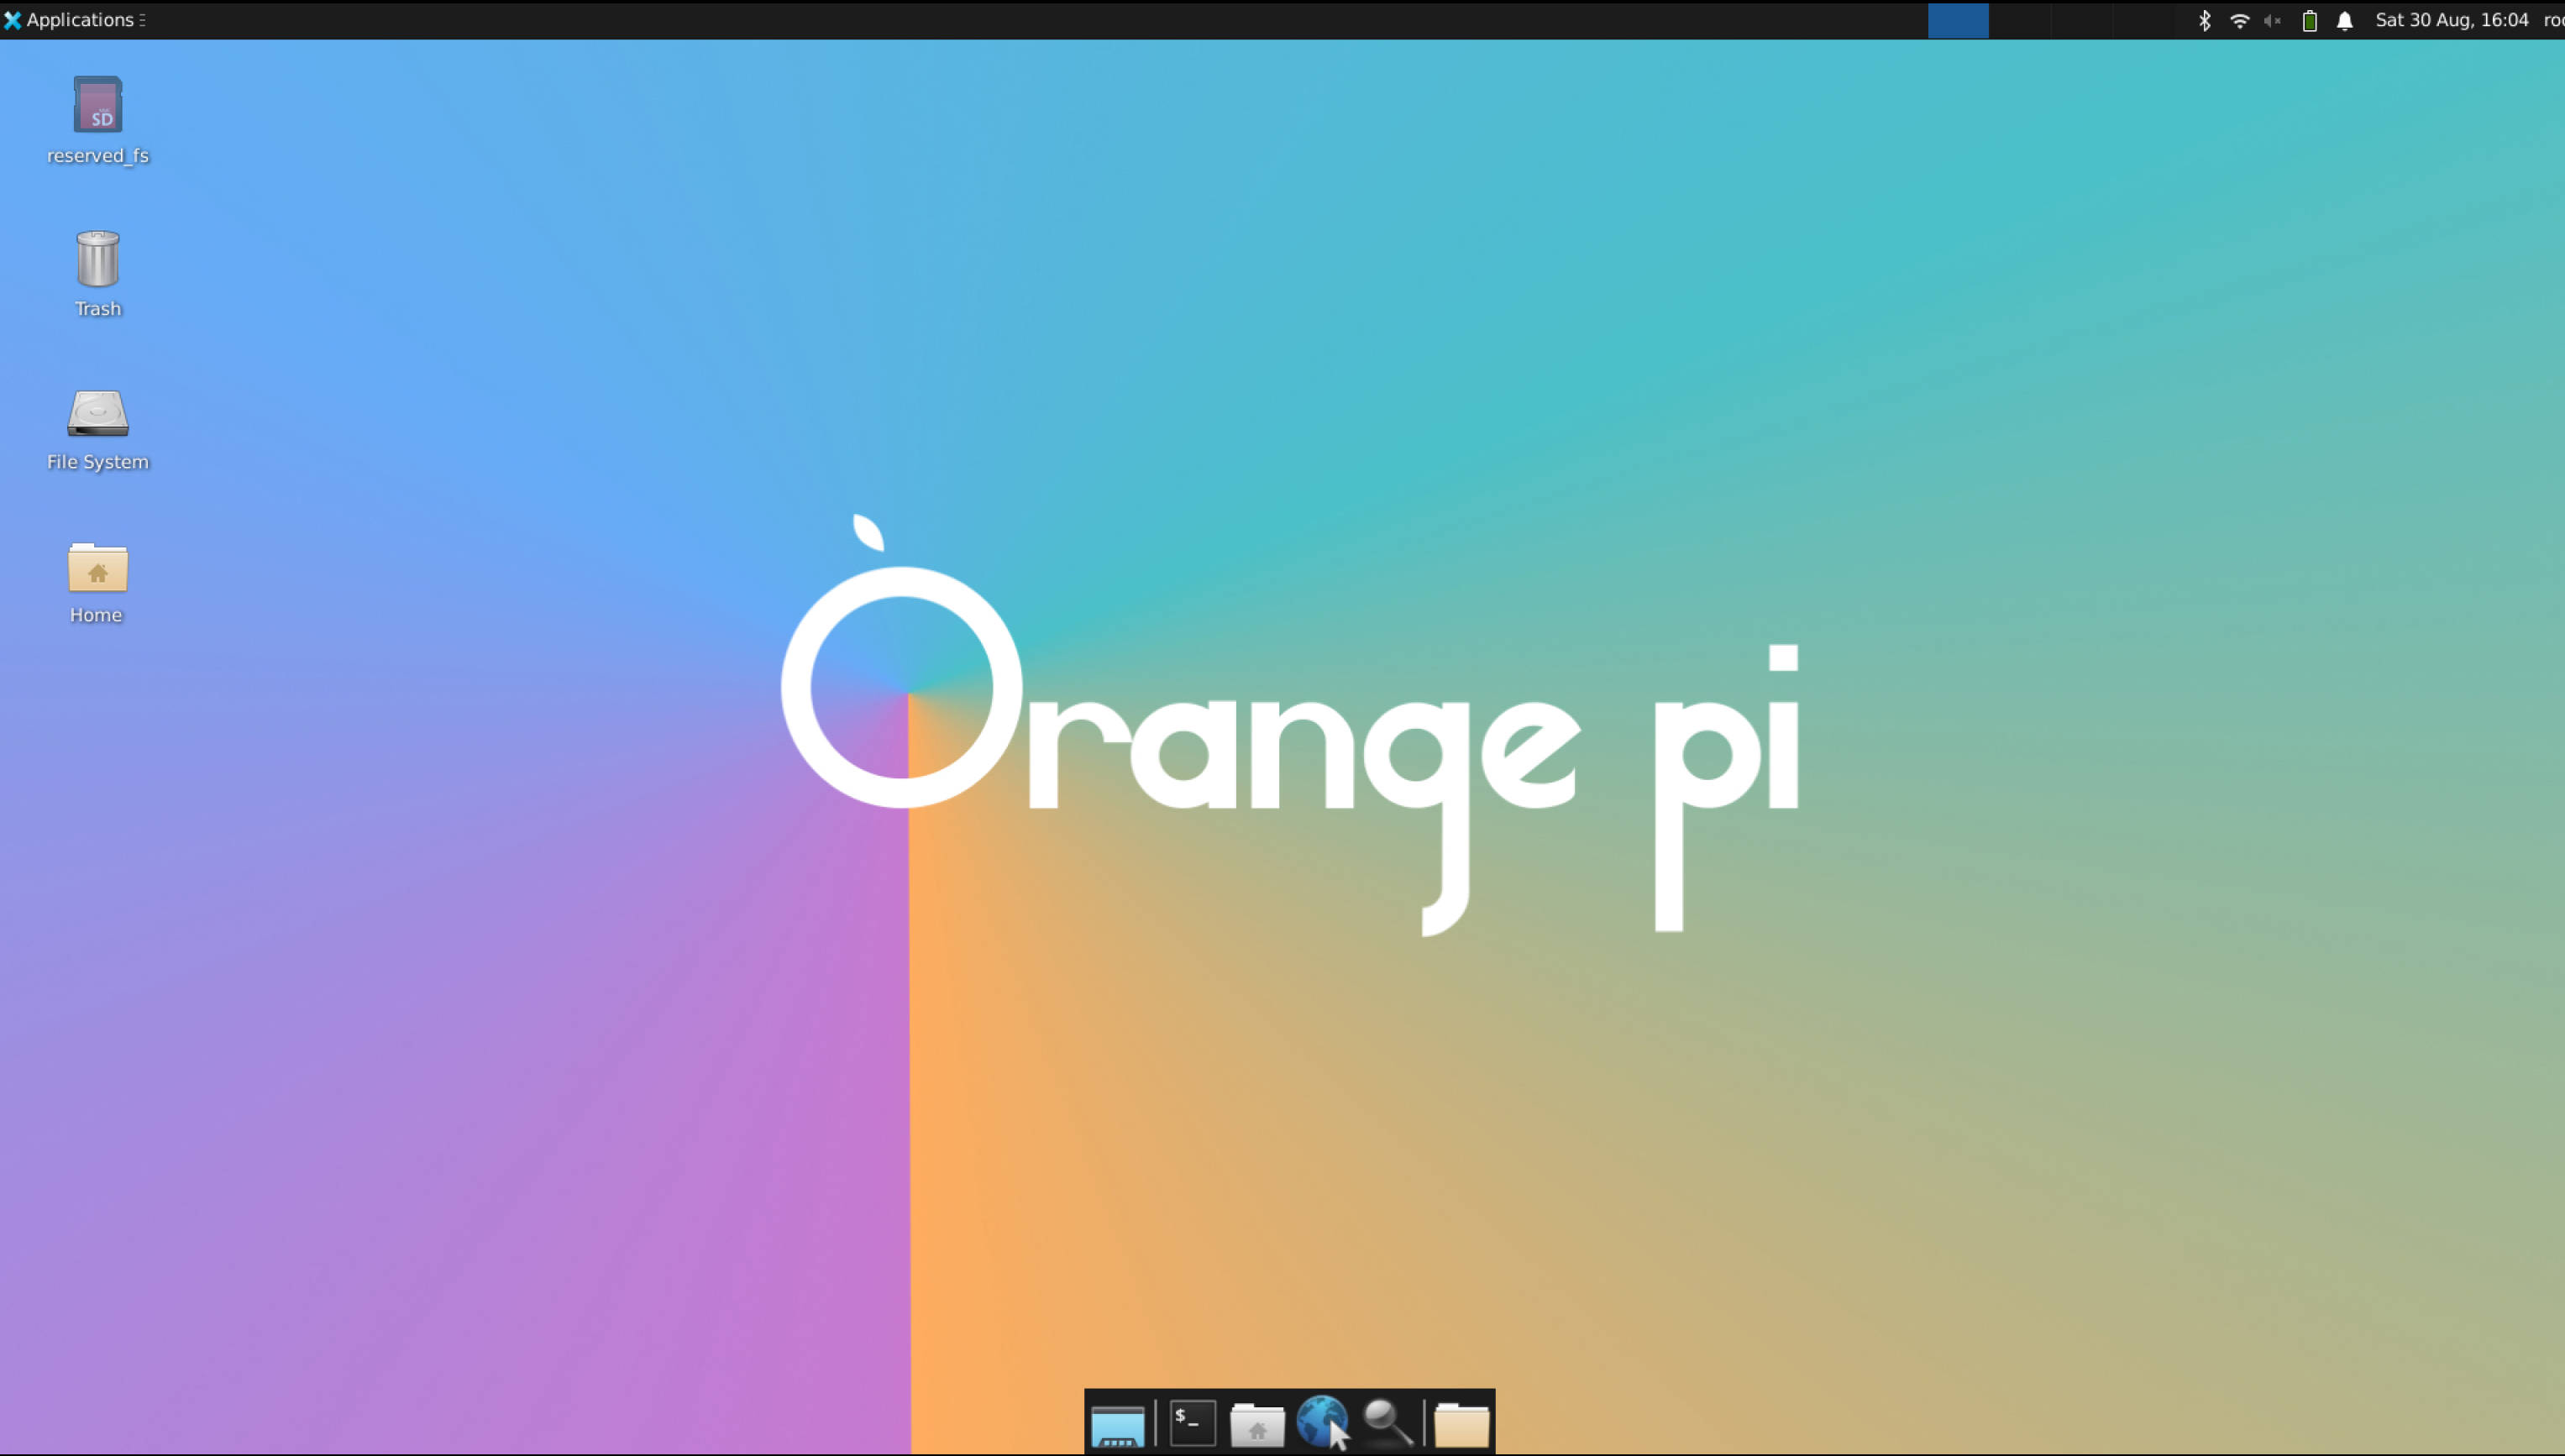
\includegraphics{img1/logingui.png} 默认账户表格: \textbar{} 用户名
  \textbar{} 密码 \textbar{} \textbar{} :---: \textbar{} :--: \textbar{}
  \textbar{} root \textbar{} Mind@123 \textbar{} \textbar{} HwHiAiUser
  \textbar{} Mind@123 \textbar{}
\end{enumerate}

\begin{itemize}
\tightlist
\item
  串口界面
\end{itemize}

\begin{enumerate}
\def\labelenumi{\arabic{enumi}.}
\tightlist
\item
  使用USB2TTL模块,与开发板的GPIO口进行连线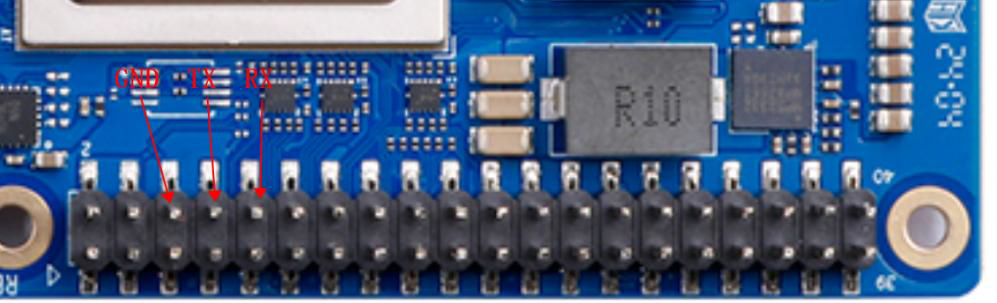
\includegraphics{img1/gpio_ttl.png},开发板的TX(GPIO8)接入USB2TTL模块的RX接口,开发板的RX(GPIO10)则接入模块的TX接口,并连接好GND接地,在Windows电脑下可以使用PUTTY连接串口。
\item
  使用开发板自带的Micro
  USB接口进行串口调试,该方法更为方便,只需要一根Micro
  USB数据线,接入电脑后打开设备管理器查询对应的串口,然后使用PUTTY进行链接即可。
  以Micro USB接口为例:
\item
  使用Micro USB数据线连接开发板和电脑
\item
  打开电脑的设备管理器,选择端口,寻找开发板对应的串口端口号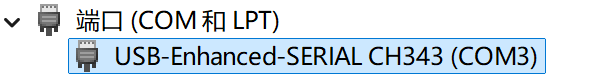
\includegraphics{img1/ttl.png}
\item
  打开串口调试软件(PUTTY)\includegraphics{img1/putty.png},将Connection
  Type选择为\texttt{Serial},然后在Serial
  Line处将端口号修改为设备管理器中查到的端口号,如作者此处端口号为\texttt{COM3},此外,还需要将Speed从9600修改为115200,最后点击Open打开串口。
\item
  等待出现\texttt{Ubuntu\ 22.04.3\ LTS\ orangepiaipro\ ttyAM0}字样,输入登录的用户名HwHiAiUser并回车,然后输入密码Mind@123并回车,注意在输入密码的时候屏幕并不会显示任何东西,登陆后的界面如图所示。
  \includegraphics{img1/serial.png} \includegraphics{img1/login.png}
\end{enumerate}

\hypertarget{ubuntu-xfceux684cux9762ux4f7fux7528ux8bf4ux660e}{%
\subsection{Ubuntu
Xfce桌面使用说明}\label{ubuntu-xfceux684cux9762ux4f7fux7528ux8bf4ux660e}}

目前系统仅支持Ubuntu 22.04 - Jammy系统,内核版本为Linux 5.10 \#\#\#\#
当前版本适配情况
请详见香橙派官方的用户手册,有部分功能仅支持使用官方程序进行测试,无法直接从系统中调用,在使用过程中需注意这些限制。

\hypertarget{hdmiux53e3ux4f7fux7528}{%
\subsubsection{HDMI口使用}\label{hdmiux53e3ux4f7fux7528}}

开发板有两个HDMI2.0 接口,目前只有HDMI0 支持显示Linux
系统的桌面,当Linux 系统的桌面系统关闭时,HDMI0 和HDMI1 还可以用于NVR
二次开 发场景输出图片。

\hypertarget{ux97f3ux9891ux4f7fux7528}{%
\subsubsection{音频使用}\label{ux97f3ux9891ux4f7fux7528}}

Linux 内核没有适配耳机和HDMI 等的ALSA 音频驱动,此部分驱动还在开
发中,目前只能通过音频样例代码来测试耳机、HDMI 的音频播放和板载MIC
的录音功能。或者自行购买Linux系统免驱的USB外置声卡,经测试可以正常使用。


% 第二章
\chapter{CANN 软件栈核心与模型转换全流程}
\section{章节总览}\label{ux7ae0ux8282ux603bux89c8}

本章系统阐述 Ascend CANN 软件栈的分层结构、模型从框架格式到 OM
的转换原理、转换工具 ATC 的关键参数、OM 文件组织结构、AscendCL (ACL)
推理编程模型、精度与性能验证方法以及工程级质量保障流水线建设。阅读完成后应满足:
1. 能解释 Driver / Runtime / Compiler / Toolkit / ACL
各组件职责及交互边界。 2. 能为任意主流视觉模型编写一份无二义性的 ATC
转换命令并说明参数意义。 3. 能通过脚本解析 OM
模型的输入输出信息、算子统计与内存占用估算。 4. 能以 C 或 Python
写出健壮的最小推理程序(含异常处理与资源释放)。 5.
能定位转换/推理常见错误,给出复现、分析与修复路径。 6. 能构建``转换 →
精度对齐 → 性能基线 → 回归监测''的自动流水线。

\section{CANN
软件栈分层与数据流}\label{cann-ux8f6fux4ef6ux6808ux5206ux5c42ux4e0eux6570ux636eux6d41}

\begin{longtable}[]{@{}
  >{\raggedright\arraybackslash}p{(\linewidth - 6\tabcolsep) * \real{0.1667}}
  >{\raggedright\arraybackslash}p{(\linewidth - 6\tabcolsep) * \real{0.1667}}
  >{\raggedright\arraybackslash}p{(\linewidth - 6\tabcolsep) * \real{0.3333}}
  >{\raggedright\arraybackslash}p{(\linewidth - 6\tabcolsep) * \real{0.3333}}@{}}
\toprule\noalign{}
\begin{minipage}[b]{\linewidth}\raggedright
层级
\end{minipage} & \begin{minipage}[b]{\linewidth}\raggedright
组件
\end{minipage} & \begin{minipage}[b]{\linewidth}\raggedright
核心职责
\end{minipage} & \begin{minipage}[b]{\linewidth}\raggedright
典型交互
\end{minipage} \\
\midrule\noalign{}
\endhead
\bottomrule\noalign{}
\endlastfoot
硬件抽象 & Driver & 设备初始化、资源枚举、功耗/温度接口 & npu-smi /
Runtime \\
运行时 & Runtime & 上下文(Context)管理、Stream/Task 调度、内存分配 & ACL
/ Compiler \\
编译优化 & Graph Compiler &
图解析、拓扑排序、算子匹配、内存复用、算子融合 & ATC / Runtime \\
工具链 & Toolkit & ATC 转换、Profiling、Dump、可视化、日志 & 开发者 \\
API 层 & AscendCL & C 接口封装:模型管理 / 内存 / 数据传输 / 执行 &
应用 \\
\end{longtable}

数据流(框架模型 → OM → 推理)核心阶段: 1. 前端导出:PyTorch →
ONNX(维度常量化、算子展开)。 2. ATC 编译:图解析 → Shape Infer →
算子选择 → Kernel 排布 → 内存映射 → 生成 OM(二进制 + 元数据段)。 3.
运行加载:aclmdlLoadFromFile 读取 OM Header,分配 Device
内存,构建执行计划(Task 列表)。 4. 推理执行:Host 侧准备输入 → H2D
拷贝 → Runtime 提交 Task → 硬件执行 → D2H 拷贝 → 后处理。

\section{环境一致性与安装验证}\label{ux73afux5883ux4e00ux81f4ux6027ux4e0eux5b89ux88c5ux9a8cux8bc1}

环境差异是隐性失败根源,建议形成``安装后自检''脚本,校验以下要点: 1.
版本矩阵:固件/Driver/CANN/ATC 必须在官方 Release Note 支持组合内。 2.
环境变量:\passthrough{\lstinline!ASCEND\_INSTALL\_PATH!}
指向安装根;\passthrough{\lstinline!LD\_LIBRARY\_PATH!} 中包含
\passthrough{\lstinline!driver!} 与
\passthrough{\lstinline!runtime/lib64!};Python 绑定需在
\passthrough{\lstinline!PYTHONPATH!} 中。 3.
设备可见:\passthrough{\lstinline!npu-smi info!} 返回芯片型号
\passthrough{\lstinline!Ascend310B!} 且状态正常,无
\passthrough{\lstinline!Fault!} 标记。 4.
转换工具:\passthrough{\lstinline!atc --version!}
输出版本与期望匹配;\passthrough{\lstinline!atc --help!}
能正常列出参数。 5. 运行权限:当前用户具备访问
\passthrough{\lstinline!/dev/davinci*!}
设备节点读写权限(若无,加入相应用户组或 udev 规则)。 6. Python
依赖:\passthrough{\lstinline!numpy!}, \passthrough{\lstinline!onnx!},
\passthrough{\lstinline!onnxruntime!} (精度对齐),
\passthrough{\lstinline!pyyaml!}, 自编写工具包。

\section{模型准备与输入规范统一}\label{ux6a21ux578bux51c6ux5907ux4e0eux8f93ux5165ux89c4ux8303ux7edfux4e00}

\begin{longtable}[]{@{}lll@{}}
\toprule\noalign{}
项 & 说明 & 决策标准 \\
\midrule\noalign{}
\endhead
\bottomrule\noalign{}
\endlastfoot
边界 Shape & 静态 or 动态 & 场景多尺寸/Batch 波动? \\
Layout & NCHW / NHWC & 上游预处理 \& 算子最佳实现 \\
颜色空间 & RGB / BGR / YUV & 原始采集格式 + 算子期望 \\
归一化 & mean/std / scale & 训练环节定义必须完全对齐 \\
精度策略 & FP16 / INT8 & 性能目标 \& 可接受精度损失 \\
Quant 校准集 & 代表性样本 & 覆盖亮度/场景/尺寸多样性 \\
\end{longtable}

核心风险:训练与部署输入不一致(尺寸拉伸方式、通道顺序、归一化顺序、色彩空间转换位置)。必须输出``输入契约文件''(JSON/YAML)标注:\passthrough{\lstinline!shape!}、\passthrough{\lstinline!dtype!}、\passthrough{\lstinline!layout!}、\passthrough{\lstinline!color\_space!}、\passthrough{\lstinline!mean/std!}、\passthrough{\lstinline!range!}、\passthrough{\lstinline!precision\_mode!}。

\section{ATC
模型转换详解}\label{atc-ux6a21ux578bux8f6cux6362ux8be6ux89e3}

典型命令(以 ResNet50 为例,支持 FP16):

\begin{lstlisting}
atc \
  --model=resnet50.onnx \
  --framework=5 \
  --output=resnet50_fp16 \
  --input_format=NCHW \
  --input_shape="input:1,3,224,224" \
  --soc_version=Ascend310B \
  --precision_mode=allow_fp32_to_fp16 \
  --op_select_implmode=high_performance \
  --log=info \
  --insert_op_conf=aipp.cfg
\end{lstlisting}

关键参数说明: \textbar{} 参数 \textbar{} 作用 \textbar{} 注意事项
\textbar{} \textbar{} ---- \textbar{} ---- \textbar{} --------
\textbar{} \textbar{} \passthrough{\lstinline!--framework!} \textbar{}
输入框架类型 (5=ONNX) \textbar{} 与实际导出一致,否则形状推理异常
\textbar{} \textbar{} \passthrough{\lstinline!--input\_shape!}
\textbar{} 静态 shape 指定 \textbar{} 多输入以逗号分隔
\passthrough{\lstinline!in1:1,3,224,224;in2:1,128!} \textbar{}
\textbar{} \passthrough{\lstinline!--dynamic\_batch\_size!} \textbar{}
动态 Batch \textbar{} 与 \passthrough{\lstinline!--input\_shape!}
不能混用静态冲突 \textbar{} \textbar{}
\passthrough{\lstinline!--dynamic\_image\_size!} \textbar{} 动态分辨率
\textbar{} YOLO 等多尺度部署 \textbar{} \textbar{}
\passthrough{\lstinline!--precision\_mode!} \textbar{} 精度策略
\textbar{}
\passthrough{\lstinline!allow\_mix\_precision!}、\passthrough{\lstinline!allow\_fp32\_to\_fp16!}
\textbar{} \textbar{} \passthrough{\lstinline!--soc\_version!}
\textbar{} 硬件目标 \textbar{} 与实际芯片匹配;310B 与 310P 不可混淆
\textbar{} \textbar{} \passthrough{\lstinline!--insert\_op\_conf!}
\textbar{} AIPP(预处理) \textbar{} 可下沉色彩空间转换、均值/方差
\textbar{} \textbar{} \passthrough{\lstinline!--op\_select\_implmode!}
\textbar{} 算子实现优先级 \textbar{}
\passthrough{\lstinline!high\_precision!} vs
\passthrough{\lstinline!high\_performance!} \textbar{} \textbar{}
\passthrough{\lstinline!--input\_format!} \textbar{} 模型输入排布
\textbar{} 与 \passthrough{\lstinline!--input\_shape!} 一致性检查
\textbar{} \textbar{} \passthrough{\lstinline!--output\_type!}
\textbar{} 输出 dtype \textbar{} 常用于 INT8 推理后转 FP32 便于后处理
\textbar{} \textbar{} \passthrough{\lstinline!--enable\_small\_channel!}
\textbar{} 小通道优化 \textbar{} 某些轻量网络加速 \textbar{}

\subsection{自定义算子加载}\label{ux81eaux5b9aux4e49ux7b97ux5b50ux52a0ux8f7d}

\begin{enumerate}
\def\labelenumi{\arabic{enumi}.}
\tightlist
\item
  定义 JSON 描述(输入输出、属性)。
\item
  编写 Kernel 源码并使用官方编译脚本生成 \passthrough{\lstinline!.so!}。
\item
  ATC 阶段通过 \passthrough{\lstinline!--optypelist\_for\_impl!} 或
  \passthrough{\lstinline!--soc\_version!} + JSON 注册;运行时放置在
  \passthrough{\lstinline!ASCEND\_OPP\_PATH!} 对应目录。
\end{enumerate}

\subsection{日志与告警}\label{ux65e5ux5fd7ux4e0eux544aux8b66}

常见告警分类: - 未使用节点 (prune) → 确认是否为训练辅助算子 (e.g.,
Dropout)。 - 算子降级 → 检查是否 fallback 到
Host;对性能敏感需重写/替换结构。 - 精度截断 →
记录发生算子,评估对最终指标影响;必要时关闭相关优化策略。

\section{OM 文件结构解读}\label{om-ux6587ux4ef6ux7ed3ux6784ux89e3ux8bfb}

OM 通常包含: 1. Header:魔数、版本、输入输出 Tensor
数、DataType、Format。 2. Graph
Meta:节点拓扑、算子类型列表、权重偏移指针。 3. Weights
Segment:连续存放常量权重与常量张量。 4. Task List:调度指令列表(Kernel
Launch / MemCopy / Event)。 5. AIPP 配置(可选):预处理算子参数表。

\subsection{解析与统计脚本要点}\label{ux89e3ux6790ux4e0eux7edfux8ba1ux811aux672cux8981ux70b9}

\begin{itemize}
\tightlist
\item
  调用 \passthrough{\lstinline!aclmdlQuerySize!}
  得到模型工作内存与权重内存需求。
\item
  利用 \passthrough{\lstinline!aclmdlGetInputIndexByName!} /
  \passthrough{\lstinline!aclmdlGetInputDims!} 获取 IO 维度与 dtype。
\item
  自建表格:\passthrough{\lstinline!\{op\_type: count\}!}
  用于识别热点类型(后续优化参考)。
\end{itemize}

\section{ACL
推理编程模型}\label{acl-ux63a8ux7406ux7f16ux7a0bux6a21ux578b}

典型生命周期: 1. 初始化:\passthrough{\lstinline!aclInit!} →
\passthrough{\lstinline!aclrtSetDevice!} →
\passthrough{\lstinline!aclrtCreateContext!} → (可选) 创建 Stream。 2.
模型:\passthrough{\lstinline!aclmdlLoadFromFile!} → 查询 IO 描述 →
预分配 Device Buffer。 3. 数据准备:Host 侧申请内存(Pinned 优先)→
格式/归一化 → H2D 拷贝。 4.
执行:\passthrough{\lstinline!aclmdlExecute!} 或 异步
\passthrough{\lstinline!aclmdlExecuteAsync!} + Stream 同步。 5.
输出处理:D2H 拷贝 → 解码 / Softmax / NMS。 6.
资源释放:\passthrough{\lstinline!aclmdlUnload!} → Free buffers →
Destroy Context → \passthrough{\lstinline!aclFinalize!}。

\subsection{C
语言最小示例(核心片段)}\label{c-ux8bedux8a00ux6700ux5c0fux793aux4f8bux6838ux5fc3ux7247ux6bb5}

\begin{lstlisting}
// 省略错误检查宏定义 ERR_CHK
aclInit(NULL);
aclrtSetDevice(0);
aclrtContext ctx; aclrtCreateContext(&ctx, 0);
uint32_t modelId; size_t wSize, rSize;
aclmdlLoadFromFile("resnet50_fp16.om", &modelId);
aclmdlDesc *desc = aclmdlCreateDesc();
aclmdlGetDesc(desc, modelId);
// 输入准备
void *hostIn = malloc(3*224*224*2); // FP16
void *devIn; aclrtMalloc(&devIn, 3*224*224*2, ACL_MEM_MALLOC_NORMAL_ONLY);
aclrtMemcpy(devIn, 3*224*224*2, hostIn, 3*224*224*2, ACL_MEMCPY_HOST_TO_DEVICE);
aclmdlDataset *input = aclmdlCreateDataset();
aclDataBuffer *inBuf = aclCreateDataBuffer(devIn, 3*224*224*2);
aclmdlAddDatasetBuffer(input, inBuf);
// 输出
size_t outSize = 1000 * 2; // FP16 logits
void *devOut; aclrtMalloc(&devOut, outSize, ACL_MEM_MALLOC_NORMAL_ONLY);
aclmdlDataset *output = aclmdlCreateDataset();
aclDataBuffer *outBuf = aclCreateDataBuffer(devOut, outSize);
aclmdlAddDatasetBuffer(output, outBuf);
aclmdlExecute(modelId, input, output);
// 回拷
void *hostOut = malloc(outSize);
aclrtMemcpy(hostOut, outSize, devOut, outSize, ACL_MEMCPY_DEVICE_TO_HOST);
// 解析 softmax ...
// 清理省略
\end{lstlisting}

\subsection{Python 封装思路}\label{python-ux5c01ux88c5ux601dux8def}

官方 Python 包接口层次相似,建议封装
\passthrough{\lstinline!ModelSession!} 类:

\begin{lstlisting}
class ModelSession:
    def __init__(self, om_path):
        self.model_id = load(om_path)
        self.desc = query(self.model_id)
        self._alloc_io_buffers()
    def infer(self, np_input: np.ndarray):
        # preprocess -> copy H2D -> execute -> copy D2H -> postprocess
        return logits
    def __del__(self):
        self._release()
\end{lstlisting}

\section{性能与初步调优策略}\label{ux6027ux80fdux4e0eux521dux6b65ux8c03ux4f18ux7b56ux7565}

\begin{longtable}[]{@{}llll@{}}
\toprule\noalign{}
问题 & 诊断信号 & 初级优化 & 进阶优化 \\
\midrule\noalign{}
\endhead
\bottomrule\noalign{}
\endlastfoot
时延波动大 & P95 \textgreater\textgreater{} P50 & 固定 Batch / 预热 &
Stream 并行 + Pin 内存 \\
吞吐不足 & 利用率低 & FP16 & 多实例并行 \\
拷贝过多 & H2D 大占比 & 合并预处理 & AIPP 下沉 \\
算子退化 & 日志 Fallback & 替换模型结构 & 自定义算子 \\
\end{longtable}

关键早期收集指标:平均时延、P95、H2D+Pre
占比、推理核心阶段占比、内存峰值。

\section{常见错误分类与排查路径}\label{ux5e38ux89c1ux9519ux8befux5206ux7c7bux4e0eux6392ux67e5ux8defux5f84}

\begin{longtable}[]{@{}
  >{\raggedright\arraybackslash}p{(\linewidth - 8\tabcolsep) * \real{0.1250}}
  >{\raggedright\arraybackslash}p{(\linewidth - 8\tabcolsep) * \real{0.2500}}
  >{\raggedright\arraybackslash}p{(\linewidth - 8\tabcolsep) * \real{0.2500}}
  >{\raggedright\arraybackslash}p{(\linewidth - 8\tabcolsep) * \real{0.2500}}
  >{\raggedright\arraybackslash}p{(\linewidth - 8\tabcolsep) * \real{0.1250}}@{}}
\toprule\noalign{}
\begin{minipage}[b]{\linewidth}\raggedright
场景
\end{minipage} & \begin{minipage}[b]{\linewidth}\raggedright
日志/现象
\end{minipage} & \begin{minipage}[b]{\linewidth}\raggedright
根因类型
\end{minipage} & \begin{minipage}[b]{\linewidth}\raggedright
排查步骤
\end{minipage} & \begin{minipage}[b]{\linewidth}\raggedright
修复
\end{minipage} \\
\midrule\noalign{}
\endhead
\bottomrule\noalign{}
\endlastfoot
ATC Unsupported Op & E190xx & 模型含新算子 & onnxsim → 拆解 &
替换/重写 \\
动态 Shape OOM & 执行时内存溢出 & 最大分辨率超预算 & 统计输入分布 &
分桶/裁剪 \\
精度下降 & Top1 -5\% & 归一化差异 & 离线对齐脚本 & 修正预处理 \\
输出 NAN & logits 异常 & 上溢/量化尺度错误 & Dump 中间 Tensor &
重新校准 \\
设备不可见 & aclInit 失败 & Driver 未加载 & dmesg \& npu-smi &
重装驱动 \\
\end{longtable}

\section{质量保障与自动化流水线}\label{ux8d28ux91cfux4fddux969cux4e0eux81eaux52a8ux5316ux6d41ux6c34ux7ebf}

流水线阶段: 1. Export:框架导出 + ONNX Simplify +
模型签名(\passthrough{\lstinline!inputs/name/dtype/layout/mean/std!}).
2. Convert:ATC 命令模板参数化(YAML → 渲染)。 3. Validate:ONNXRuntime
vs OM 输出差异 (L1/L2/TopK 差异率 \textless{} 阈值)。 4.
Benchmark:Warmup N + Run M,记录 JSON
\passthrough{\lstinline!\{avg, p50, p95, memory\}!}。 5.
Archive:产物归档(om, atc.log, metrics.json, signature.json)。 6.
Regression:新提交对比基线差异,超阈值报警。

\subsection{精度对齐示例指标}\label{ux7cbeux5ea6ux5bf9ux9f50ux793aux4f8bux6307ux6807}

\begin{longtable}[]{@{}lll@{}}
\toprule\noalign{}
指标 & 计算方式 & 推荐阈值 \\
\midrule\noalign{}
\endhead
\bottomrule\noalign{}
\endlastfoot
Top1 差异 & abs(top1\_acc\_onnx - top1\_acc\_om) & ≤0.2\% \\
平均 L1 & mean( & y\_onnx - y\_om \\
最大相对误差 & max( & d \\
\end{longtable}

\section{Dump / Profiling /
调试手段}\label{dump-profiling-ux8c03ux8bd5ux624bux6bb5}

\begin{longtable}[]{@{}llll@{}}
\toprule\noalign{}
工具 & 使用时机 & 价值 & 代价 \\
\midrule\noalign{}
\endhead
\bottomrule\noalign{}
\endlastfoot
Dump 中间 Tensor & 精度异常 & 对齐中间层 & I/O 与存储占用 \\
Profiling Timeline & 性能不达标 & 定位瓶颈 & 额外开销 (W\%) \\
日志级别升高 (\passthrough{\lstinline!--log=debug!}) & 转换失败 &
细粒度错误码 & 噪声多 \\
校准数据捕获 & INT8 偏差大 & 重新校准 & 需准备代表性样本 \\
\end{longtable}

Dump 配置:通过环境变量或 JSON 指定层名称白名单,避免全量 Dump
导致性能与空间压力。

\section{动态 Shape
策略与内存规划}\label{ux52a8ux6001-shape-ux7b56ux7565ux4e0eux5185ux5b58ux89c4ux5212}

多分辨率/Batch 场景建议: 1. 分桶:统计历史尺寸 → 选 3\textasciitilde5
个``代表桶'' → ATC 生成多 OM;运行时按最近桶选择。 2. Padding:对齐到
32/64 边界,减少算子内部分支;记录真实尺寸用于后处理。 3.
内存预估:最大桶内存 + 安全冗余 15\% 作为部署阈值,超出触发降级。

\section{精度验证流程与脚本要点}\label{ux7cbeux5ea6ux9a8cux8bc1ux6d41ux7a0bux4e0eux811aux672cux8981ux70b9}

流程:采样输入集(校准集或验证集子集)→ ONNXRuntime 前向 → Ascend 前向 →
指标聚合 → 报告。 脚本关键: 1. 随机种子固定; 2.
输入预处理完全共用函数; 3. 支持逐层 Dump 比对(差异 \textgreater{} 阈值
输出层名)。

\section{安全与合规考量}\label{ux5b89ux5168ux4e0eux5408ux89c4ux8003ux91cf}

\begin{itemize}
\tightlist
\item
  模型资产:带版权或敏感权重需加密存储(考虑文件系统权限+传输校验
  hash)。
\item
  日志脱敏:避免输出用户数据路径/片段;开关化控制。
\item
  Dump
  数据:限定开发模式,生产禁用;数据自动过期删除策略(时间或数量)。
\end{itemize}

\section{章节小结}\label{ux7ae0ux8282ux5c0fux7ed3}

本章从宏观分层、转换编译、OM 结构、ACL
编程、性能与精度保障、调试工具、自动化流水线到动态 Shape
与安全实践建立了闭环。掌握这些内容后即可进入后续``边缘系统架构与部署实践''章节,扩展到多模型、多进程及系统级优化。

\section{实践任务}\label{ux5b9eux8df5ux4efbux52a1}

\begin{enumerate}
\def\labelenumi{\arabic{enumi}.}
\tightlist
\item
  任选一个公开 ONNX 分类模型(如 ResNet50)完成 ATC 转换,提交:命令 +
  atc.log。
\item
  以 C 或 Python 实现最小推理程序,输出前 5 TopK 结果与 softmax 概率。
\item
  编写对齐脚本比较 50 张图片 ONNX vs OM 输出差异(报告 L1/Top1 差异)。
\item
  收集 Profiling Timeline,列出前 3 耗时算子类型及优化建议。
\item
  输出
  \passthrough{\lstinline!signature.json!}、\passthrough{\lstinline!metrics.json!}、\passthrough{\lstinline!conversion\_meta.yaml!}
  并归档。
\end{enumerate}


% 第三章
\chapter{昇腾310B算子开发基础}
昇腾310B在通用算子覆盖广度上已能满足大多数推理任务,但在以下场景,自定义算子(Custom
Op)能显著提升功能完备性与性能确定性:模型含未支持/半支持算子、复合算子频繁导致访存过多、需要业务特化(如阈值/形态学/后处理融合)、或内置实现对特定尺寸/布局性能欠佳。第三章将给出``为什么、怎么做、如何验证与上线''的完整路径。

\section{算子开发概述}\label{ux7b97ux5b50ux5f00ux53d1ux6982ux8ff0}

\begin{itemize}
\tightlist
\item
  目标与收益:

  \begin{itemize}
  \tightlist
  \item
    功能补齐:覆盖模型图中未支持或语义差异较大的算子;
  \item
    性能确定性:融合多算子、减少GM\textless-\textgreater UB搬运与中间落地、利用向量化内核;
  \item
    工程可维护:以``算子契约''形式固化输入/输出/属性与边界行为,便于回归与复用。
  \end{itemize}
\item
  执行形态:

  \begin{itemize}
  \tightlist
  \item
    AI Core(推荐):基于 TBE/TE/TIK 运行于 NPU 核心,适合数值密集型;
  \item
    AICPU(可选):C/C++ 在 AICPU/Host
    侧执行,适合控制流/轻量处理(注意H2D/D2H成本)。
  \end{itemize}
\item
  产物要素:

  \begin{itemize}
  \tightlist
  \item
    算子描述(op info/proto):声明
    op\_type、inputs/outputs、dtype\_format 组合、属性与形状推断;
  \item
    算子实现(Kernel):TE/TIK 计算+调度或 AICPU C++ 实现;
  \item
    注册与打包:产物按规范放入 OPP 目录,ATC/Runtime 可发现与加载。
  \end{itemize}
\end{itemize}

\section{开发的理论基础}\label{ux5f00ux53d1ux7684ux7406ux8bbaux57faux7840}

\begin{enumerate}
\def\labelenumi{\arabic{enumi})}
\tightlist
\item
  硬件与存储层次:
\end{enumerate}

\begin{itemize}
\tightlist
\item
  GM(Global Memory):容量大、带宽高;
\item
  UB(Unified Buffer):片上高速缓存,容量有限;
\item
  DMA:GM↔UB 的数据搬运,偏好大块连续传输;
\item
  向量/标量单元:支持vadd/vmul/vmax等,需数据对齐(常见16/32)。
\end{itemize}

\begin{enumerate}
\def\labelenumi{\arabic{enumi})}
\setcounter{enumi}{1}
\tightlist
\item
  计算表达与调度:
\end{enumerate}

\begin{itemize}
\tightlist
\item
  TE(Tensor Expression)描述计算公式;Schedule 负责
  tile/并行/向量化/缓存;
\item
  TIK 提供更贴近硬件的 DSL,便于精细控制 DMA 与 UB 管理;
\item
  目标:以较少的GM往返在UB内完成尽可能多的计算,提升算子算子效率与吞吐。
\end{itemize}

\begin{enumerate}
\def\labelenumi{\arabic{enumi})}
\setcounter{enumi}{2}
\tightlist
\item
  算子契约(Operator Contract):
\end{enumerate}

\begin{itemize}
\tightlist
\item
  输入/输出张量的
  shape、dtype、layout(NCHW/NC1HWC0等)、属性(如alpha、mode);
\item
  广播与对齐规则、边界行为(溢出/饱和/舍入)、精度策略(FP16/FP32混合);
\item
  动态shape与静态shape:实现需覆盖契约内的形状组合并保证UB不溢出。
\end{itemize}

\begin{enumerate}
\def\labelenumi{\arabic{enumi})}
\setcounter{enumi}{3}
\tightlist
\item
  数值与精度:
\end{enumerate}

\begin{itemize}
\tightlist
\item
  FP16 常用于 310B 推理通路;必要时在关键步骤采用临时 FP32 计算再回写;
\item
  误差控制:选择合适的舍入策略,避免饱和/下溢导致NAN/INF。
\end{itemize}

\section{开发流程(AI Core
路线)}\label{ux5f00ux53d1ux6d41ux7a0bai-core-ux8defux7ebf}

\begin{enumerate}
\def\labelenumi{\arabic{enumi}.}
\tightlist
\item
  环境准备与约束
\end{enumerate}

\begin{itemize}
\tightlist
\item
  安装 CANN/Toolkit 并确认 \passthrough{\lstinline!atc --version!}
  正常;
\item
  设置环境变量:\passthrough{\lstinline!ASCEND\_INSTALL\_PATH!}、\passthrough{\lstinline!ASCEND\_OPP\_PATH!};
\item
  目标芯片:\passthrough{\lstinline!soc\_version=Ascend310B!};优先使用
  FP16 与硬件友好布局(如NC1HWC0)。
\end{itemize}

\begin{enumerate}
\def\labelenumi{\arabic{enumi}.}
\setcounter{enumi}{1}
\tightlist
\item
  定义算子信息(op info/proto)
\end{enumerate}

\begin{itemize}
\tightlist
\item
  声明 \passthrough{\lstinline!op\_type!}、inputs/outputs
  名称与数量、可支持的 \passthrough{\lstinline!dtype\_format!}
  组合、属性与默认值;
\item
  提供形状推断规则(静态或依据属性/输入维度计算)。
\end{itemize}

\begin{enumerate}
\def\labelenumi{\arabic{enumi}.}
\setcounter{enumi}{2}
\tightlist
\item
  编写算子实现(TE/TBE/TIK)
\end{enumerate}

\begin{itemize}
\tightlist
\item
  计算表达(示例:Add+ReLU 融合伪代码):
\end{itemize}

\begin{lstlisting}
# y = relu(x1 + x2)
import te.lang.cce as tbe
from te import tvm

def add_relu_compute(x1, x2):
        y = tbe.vadd(x1, x2)
        z = tbe.vmaxs(y, tvm.const(0.0, x1.dtype))
        return z
\end{lstlisting}

\begin{itemize}
\tightlist
\item
  调度要点:

  \begin{itemize}
  \tightlist
  \item
    Tile 到 UB 容量可承载的块大小;
  \item
    连续向量访问,减少非对齐;
  \item
    合并搬运,避免频繁小块 DMA;
  \item
    小尺寸路径避免调度开销超过计算开销。
  \end{itemize}
\end{itemize}

\begin{enumerate}
\def\labelenumi{\arabic{enumi}.}
\setcounter{enumi}{3}
\tightlist
\item
  编译与注册
\end{enumerate}

\begin{itemize}
\tightlist
\item
  使用 Toolkit 提供的编译入口生成 kernel 与元数据;
\item
  将实现与描述文件放入 \passthrough{\lstinline!ASCEND\_OPP\_PATH!} 下
  custom 目录(如
  \passthrough{\lstinline!op\_impl/custom/ai\_core/tbe!}、\passthrough{\lstinline!op\_proto/custom!})。
\end{itemize}

\begin{enumerate}
\def\labelenumi{\arabic{enumi}.}
\setcounter{enumi}{4}
\tightlist
\item
  与 ATC 集成
\end{enumerate}

\begin{itemize}
\tightlist
\item
  转换模型时指定 \passthrough{\lstinline!--soc\_version=Ascend310B!};
\item
  确保 OPP 路径可被 ATC 读取,必要时调整
  \passthrough{\lstinline!--op\_select\_implmode!};
\item
  转换日志中应能看到自定义算子被匹配与编译。
\end{itemize}

\begin{enumerate}
\def\labelenumi{\arabic{enumi}.}
\setcounter{enumi}{5}
\tightlist
\item
  运行时部署
\end{enumerate}

\begin{itemize}
\tightlist
\item
  目标环境包含同版本 OPP(含 custom 产物);
\item
  设置环境变量使 Runtime 能定位到自定义实现;
\item
  按常规 ACL 流程加载 OM 并执行推理。
\end{itemize}

\begin{enumerate}
\def\labelenumi{\arabic{enumi}.}
\setcounter{enumi}{6}
\tightlist
\item
  验证与度量
\end{enumerate}

\begin{itemize}
\tightlist
\item
  功能:与 NumPy/ONNX
  参考实现对齐,随机多组张量比较(平均绝对/相对误差、边界样本);
\item
  性能:Warmup≥3 次,采样≥50 次,统计 avg/p95/FPS;
\item
  资源:Profiling 检查 MemCopy 占比、Kernel 占比、Idle;
\item
  兼容:覆盖不同 shape/dtype/layout 组合。
\end{itemize}

\begin{enumerate}
\def\labelenumi{\arabic{enumi}.}
\setcounter{enumi}{7}
\tightlist
\item
  打包与版本化
\end{enumerate}

\begin{itemize}
\tightlist
\item
  输出 \passthrough{\lstinline!op\_contract.yaml!}(契约)与
  \passthrough{\lstinline!benchmark.json!}(性能);
\item
  目录建议:
\end{itemize}

\begin{lstlisting}
op_pkg/<op_type>/<version>/
    ├─ op_proto/custom/
    ├─ op_impl/custom/ai_core/tbe/
    ├─ tests/
    └─ docs/
\end{lstlisting}

\section{常见问题与排查}\label{ux5e38ux89c1ux95eeux9898ux4e0eux6392ux67e5}

\begin{itemize}
\tightlist
\item
  ATC 提示 Unsupported Op:检查 op 描述是否生效、路径与
  \passthrough{\lstinline!soc\_version!} 是否匹配;
\item
  运行时回退(fallback):确认 \passthrough{\lstinline!dtype\_format!}
  覆盖到当前张量组合;
\item
  性能无提升:检查是否出现额外 layout 转换、tile 过小造成 DMA 频繁;
\item
  精度异常:核对归一化/广播规则、溢出与舍入策略,必要时局部切 FP32;
\item
  动态 shape OOM:缩小 tile 或分桶处理,保证 UB 与工作区不溢出。
\end{itemize}

\section{章节小结}\label{ux7ae0ux8282ux5c0fux7ed3}

自定义算子是 310B
场景下实现``功能补齐与性能确定性''的关键手段。遵循``明确契约 → 正确调度
→ 可观测验证 →
规范打包''的路径,选择计算/访存比例合适、出现频繁的目标起步,先易后难、以基线与回归保障质量与收益的可持续。

\section{实践任务}\label{ux5b9eux8df5ux4efbux52a1}

\begin{enumerate}
\def\labelenumi{\arabic{enumi}.}
\tightlist
\item
  选择你项目中的一个复合算子(例如归一化+阈值),写出算子契约草案(IO/attr/dtype\_format/边界)。
\item
  基于 TE 写出该算子的计算表达伪代码,并说明预期的 tile 与向量化策略。
\item
  在开发环境完成编译注册,将产物放入 OPP custom 目录并用一个最小模型验证
  ATC 识别。
\item
  设计功能与性能验证脚本:随机张量对齐、Warmup/采样策略、输出 avg/p95
  与资源占比。
\item
  生成 \passthrough{\lstinline!op\_contract.yaml!} 与
  \passthrough{\lstinline!benchmark.json!},并归档到
  \passthrough{\lstinline!op\_pkg/<op\_type>/<version>/!}。
\end{enumerate}


% 第四章
\chapter{典型模型部署实践}
\section{章节总览}\label{ux7ae0ux8282ux603bux89c8}

本章以``统一流程 → 四类典型任务(分类/检测/OCR/NLP)→ 多模型 Pipeline →
工程化目录与脚本 → 性能基线采集 →
问题诊断''逻辑展开,强调``可复现、可量化、可演进''的部署范式。所有示例策略均可推广到后续复杂场景(多输入、多分辨率、流式/批式混合)。

\section{统一部署工作流与契约化}\label{ux7edfux4e00ux90e8ux7f72ux5de5ux4f5cux6d41ux4e0eux5951ux7ea6ux5316}

标准六步:模型选择 → 框架导出 ONNX → ATC 转换(参数冻结)→
推理引擎封装(I/O 契约)→ 运行形态编排 → 验证(精度 + 性能)。
核心产物: \textbar{} 文件 \textbar{} 作用 \textbar{} \textbar{} ----
\textbar{} ---- \textbar{} \textbar{} export.py \textbar{} 导出 \& 简化
ONNX \textbar{} \textbar{} atc.sh \textbar{} 标准化转换命令 \textbar{}
\textbar{} config.yaml \textbar{} 输入/归一化/颜色/阈值 \textbar{}
\textbar{} signature.json \textbar{} 模型输入输出字段与 dtype \textbar{}
\textbar{} metrics.json \textbar{} 性能统计(avg/p95/memory) \textbar{}

输入预处理必须模块化,业务层仅提供原始图像对象;可在 AIPP
中下沉部分(色彩空间、均值/方差),减少 Host 侧拷贝和转换。

\section{图像分类:ResNet /
MobileNet}\label{ux56feux50cfux5206ux7c7bresnet-mobilenet}

\subsection{模型导出}\label{ux6a21ux578bux5bfcux51fa}

PyTorch →
ONNX:\passthrough{\lstinline!torch.onnx.export(model, dummy, opset\_version=13, dynamic\_axes=None)!};确保去掉训练专属层(Dropout,
BN 置 eval)。 \#\#\# 预处理一致性 1. Resize: 保持短边 256 → CenterCrop
224。 2. Normalize: mean/std 与训练保持一致。 3. Layout:
NCHW;若原始图像为 HWC(RGB) → 转 BGR/或保持一致并在 config 标记。 \#\#\#
转换要点
\passthrough{\lstinline!--precision\_mode=allow\_fp32\_to\_fp16!};若需
INT8:先做离线标定导出校准表,再加量化参数。 \#\#\# 推理后处理 Softmax →
ArgTopK → LabelMap。为避免数值不稳定:FP16 logits 可先转 FP32 再
softmax。 \#\#\# 性能采集 Warmup 5 次,采集 100 次:记录 avg, p50, p95,
max;统计预处理耗时占比:\passthrough{\lstinline!pre\_ms / total\_ms!},超过
25\% 提示 AIPP 下沉或批处理优化。

\section{目标检测:YOLO /
FasterRCNN}\label{ux76eeux6807ux68c0ux6d4byolo-fasterrcnn}

\subsection{输入尺寸与
Letterbox}\label{ux8f93ux5165ux5c3aux5bf8ux4e0e-letterbox}

Letterbox 使图像等比例缩放 +
填充,保持方形输入。部署需重现训练阶段相同逻辑,否则框坐标偏移。保存
\passthrough{\lstinline!scale!} 与 \passthrough{\lstinline!pad!}
用于反算原始坐标。 \#\#\# 多输出解析 YOLOv5s OM
输出通常包含一个或多个特征拼接张量:\passthrough{\lstinline!(num\_boxes, attributes)!};后处理:过滤
conf \textgreater{} 阈值 → 按类合并 → NMS。 \#\#\# NMS 实现决策
\textbar{} 方案 \textbar{} 优点 \textbar{} 缺点 \textbar{} \textbar{}
---- \textbar{} ---- \textbar{} ---- \textbar{} \textbar{} CPU Python
\textbar{} 简单 \textbar{} 高开销,多框场景慢 \textbar{} \textbar{} CPU
C++ SIMD \textbar{} 中等复杂 \textbar{} 仍需 D2H 拷贝 \textbar{}
\textbar{} Device Kernel \textbar{} 减少拷贝 \textbar{} 实现复杂
\textbar{} 先评估 D2H + CPU NMS 占比,\textgreater15\% 再考虑下沉。
\#\#\# 动态尺度支持 转换阶段可生成多尺度 OM 或使用动态
shape;推荐:统计输入分辨率 → 选择 3 桶(640/704/768)提升命中率。

\section{OCR:文本检测 + 识别
Pipeline}\label{ocrux6587ux672cux68c0ux6d4b-ux8bc6ux522b-pipeline}

\subsection{结构}\label{ux7ed3ux6784}

检测模型(DB) → 文本框多边形 → 透视裁剪 → 识别模型(CRNN / SVTR)。
\#\#\# 难点与策略 \textbar{} 环节 \textbar{} 风险 \textbar{} 对策
\textbar{} \textbar{} ---- \textbar{} ---- \textbar{} ---- \textbar{}
\textbar{} 多边形裁剪 \textbar{} 仿射失真 \textbar{} 统一仿射矩阵 +
padding \textbar{} \textbar{} 长短文本差异 \textbar{} 序列长度不均
\textbar{} 动态 Batch 分组(长度分桶) \textbar{} \textbar{} 识别延迟
\textbar{} 串行处理 \textbar{} 检测与上一批识别并行 \textbar{}
\textbar{} 字典映射 \textbar{} 乱码/对齐 \textbar{} 固定 vocab + 版本号
\textbar{} \#\#\# CTC 解码 贪心:移除重复与 blank;大规模需 Beam
Search(权衡性能)。

\section{NLP:BERT 推理优化}\label{nlpbert-ux63a8ux7406ux4f18ux5316}

\subsection{序列长度策略}\label{ux5e8fux5217ux957fux5ea6ux7b56ux7565}

\begin{enumerate}
\def\labelenumi{\arabic{enumi}.}
\tightlist
\item
  静态最大长度(简单,浪费算力)。
\item
  Bucketing:按输入长短分类(32/64/128/256),多 OM。
\item
  动态 shape:需评估内存分配抖动;提前预热各常见长度。 \#\#\# FP16
  注意点 LayerNorm/Softmax 数值范围敏感;若发现精度下降:保持部分算子
  FP32(通过混合精度策略或模型修改)。 \#\#\# 性能指标
  tokens/s、avg\_latency\_ms(batch=1 与
  batch\textgreater1)、内存占用;观察自注意力占比,必要时进行剪枝(去除冗余
  head)或蒸馏。
\end{enumerate}

\section{多模型 Pipeline
串联}\label{ux591aux6a21ux578b-pipeline-ux4e32ux8054}

案例:检测 → 裁剪 → 分类。 \textbar{} Stage \textbar{} 输入/输出
\textbar{} 并行策略 \textbar{} 指标采集 \textbar{} \textbar{} -----
\textbar{} -------- \textbar{} -------- \textbar{} -------- \textbar{}
\textbar{} Detector \textbar{} 原始帧 → 框 \textbar{} 批处理+单模型
\textbar{} 时延/框数 \textbar{} \textbar{} Cropper \textbar{} 帧+框 →
Patch 列表 \textbar{} 多线程 CPU \textbar{} 单 Patch 平均耗时 \textbar{}
\textbar{} Classifier \textbar{} Patch → TopK 类别 \textbar{} 合批
(N≤32) \textbar{} FPS/准确率 \textbar{} \#\#\# 优化要点 1. Buffer
池:重用图像与 Patch 内存,避免频繁 malloc。 2. 批量裁剪:收集一定数量
Patch 再统一预处理。 3. 超时控制:某帧超过阈值后续结果丢弃,保持实时性。
4. 滑窗统计:最近 60s FPS、平均队列深度。

\section{工程目录与脚本标准}\label{ux5de5ux7a0bux76eeux5f55ux4e0eux811aux672cux6807ux51c6}

\begin{lstlisting}
deploy/
  classify/
    export.py
    atc.sh
    config.yaml
  detect/
    export.py
    atc.sh
  ocr/
    export_det.py
    export_rec.py
    atc_det.sh
    atc_rec.sh
runtime/
  core/acl_session.cpp
  preprocess/
  postprocess/
  pipelines/
tests/
  data/
  benchmark/
docs/
  model_cards/
\end{lstlisting}

版本归档要求: \textbar{} 产物 \textbar{} 检查点 \textbar{} \textbar{}
---- \textbar{} ------- \textbar{} \textbar{} *.om \textbar{} 与 atc.log
hash 对应 \textbar{} \textbar{} signature.json \textbar{}
与运行时动态查询一致 \textbar{} \textbar{} metrics.json \textbar{}
包含时间戳/commit\_sha \textbar{} \textbar{} model\_card.md \textbar{}
模型来源/License/精度 \textbar{}

\section{性能基线方法与统计置信}\label{ux6027ux80fdux57faux7ebfux65b9ux6cd5ux4e0eux7edfux8ba1ux7f6eux4fe1}

推荐: 1. Warmup 5\textasciitilde10 次; 2. 收集 ≥200 次稳定样本; 3.
计算 avg, p50, p95, p99; 4.
计算置信区间:\passthrough{\lstinline!mean ± 1.96 * (std/sqrt(n))!}; 5.
记录环境:芯片序列号/温度区间/电源模式/版本矩阵。 差异判定:新版本 avg
降低 \textgreater5\% 或 p95 上升 \textgreater8\% 触发报警分析。

\section{常见问题诊断深度版}\label{ux5e38ux89c1ux95eeux9898ux8bcaux65adux6df1ux5ea6ux7248}

\begin{longtable}[]{@{}llll@{}}
\toprule\noalign{}
问题 & 表现 & 诊断步骤 & 修复 \\
\midrule\noalign{}
\endhead
\bottomrule\noalign{}
\endlastfoot
输出全 0 & logits 恒定 & Dump 中间 tensor & 校验预处理/权重损坏 \\
检测框偏移 & 坐标不准 & 可视化缩放/Pad 参数 & 修正 letterbox 逆变换 \\
OCR 乱码 & 字符错位 & 对比 index→char 映射 & 统一 vocab \& 排序 \\
BERT 性能差 & tokens/s 低 & 分析长度分布 & 分桶/裁剪长度 \\
Pipeline 堵塞 & 帧延迟增长 & 监控队列深度 & 降帧/扩线程池 \\
内存持续上涨 & long run OOM & 内存快照/工具 & 释放缓存/池化 \\
\end{longtable}

\section{章节小结}\label{ux7ae0ux8282ux5c0fux7ed3}

本章提供四类典型任务部署详解,并抽象了跨任务可复用的脚手架与性能度量方法。重点在于``输入契约统一''、``阶段解耦''、``可观察性内建''。掌握后可进入性能与算子优化专题。

\section{实践任务}\label{ux5b9eux8df5ux4efbux52a1}

\begin{enumerate}
\def\labelenumi{\arabic{enumi}.}
\tightlist
\item
  部署 ResNet50:输出 Top5 及概率、提交 metrics.json。
\item
  部署 YOLOv5s:5 张测试图片生成可视化结果(描述框坐标与类别统计)。
\item
  构建 OCR 双模型流水线:统计单帧平均文本块数 + 平均识别耗时。
\item
  BERT:对 3 组长度(32/64/128) 测 tokens/s 与时延差异,生成对比表。
\item
  Pipeline 检测→分类:实现批裁剪 + Buffer
  池,比较优化前后平均时延下降百分比。
\end{enumerate}


% 第五章
\chapter{性能与算子优化初阶}
\section{章节总览}\label{ux7ae0ux8282ux603bux89c8}

本章聚焦``定位 → 解释 → 改善''闭环:从性能分析模型、Profiling
工具、瓶颈模式分类、布局与精度策略、内存与并行调度、到自定义算子开发与验证标准,提供工程可落地方法。目标是让读者具备:A)
定量证明问题;B) 选择低风险优化策略;C) 保证功能与性能回归一致性。

\section{性能拆解与衡量框架}\label{ux6027ux80fdux62c6ux89e3ux4e0eux8861ux91cfux6846ux67b6}

总时延公式:\passthrough{\lstinline!T\_total = T\_pre + T\_h2d + T\_infer + T\_d2h + T\_post + T\_idle!}。
吞吐上限受制于 \passthrough{\lstinline!max(T\_component)!};需收集: -
平均/分位数 (p50/p95); - 波动系数 CV=std/mean(\textgreater0.15
需进一步剖析); - 稳定性:长跑 1h 是否存在漂移 (内存泄漏或热降频)。
对比优化前后必须保留固定随机种子和数据集,消除噪声。

\section{Profiling
工具与时间线解读}\label{profiling-ux5de5ux5177ux4e0eux65f6ux95f4ux7ebfux89e3ux8bfb}

关键观测元素: \textbar{} 轨迹 \textbar{} 意义 \textbar{} 异常信号
\textbar{} \textbar{} ---- \textbar{} ---- \textbar{} --------
\textbar{} \textbar{} Stream Timeline \textbar{} 内核调度顺序 \textbar{}
大量空洞 gap \textbar{} \textbar{} MemCopy \textbar{} H2D/D2H 开销
\textbar{} 频繁小块拷贝 \textbar{} \textbar{} Task Kernel \textbar{}
算子执行 \textbar{} 个别算子异常拖长 \textbar{} \textbar{} Sync/Wait
\textbar{} Host 等待 \textbar{} Wait 占比高 \textbar{}

使用策略: 1. 先全量 Profile → 定位热点范围; 2. 二次局部
Profile(过滤特定算子类型); 3. 导出 JSON → 自动解析器归档:算子耗时
TOPK,Copy 占比,Idle 时间。

\section{瓶颈模式与处置策略矩阵}\label{ux74f6ux9888ux6a21ux5f0fux4e0eux5904ux7f6eux7b56ux7565ux77e9ux9635}

\begin{longtable}[]{@{}
  >{\raggedright\arraybackslash}p{(\linewidth - 8\tabcolsep) * \real{0.1176}}
  >{\raggedright\arraybackslash}p{(\linewidth - 8\tabcolsep) * \real{0.2353}}
  >{\raggedright\arraybackslash}p{(\linewidth - 8\tabcolsep) * \real{0.2353}}
  >{\raggedright\arraybackslash}p{(\linewidth - 8\tabcolsep) * \real{0.2941}}
  >{\raggedright\arraybackslash}p{(\linewidth - 8\tabcolsep) * \real{0.1176}}@{}}
\toprule\noalign{}
\begin{minipage}[b]{\linewidth}\raggedright
模式
\end{minipage} & \begin{minipage}[b]{\linewidth}\raggedright
识别特征
\end{minipage} & \begin{minipage}[b]{\linewidth}\raggedright
定量指标
\end{minipage} & \begin{minipage}[b]{\linewidth}\raggedright
处置优先级
\end{minipage} & \begin{minipage}[b]{\linewidth}\raggedright
策略
\end{minipage} \\
\midrule\noalign{}
\endhead
\bottomrule\noalign{}
\endlastfoot
调度空洞 & Timeline gap 多 & Idle \textgreater{} 10\% & 高 & 合并小算子
/ 预加载数据 \\
访存受限 & 算子耗时与内存带宽正相关 & 算子内核利用率低 & 中 & Layout
变换 / Tile 分块 \\
H2D 瓶颈 & MemCopy 比例高 & H2D\textgreater20\% & 高 &
合并/异步/Pin/AIPP 下沉 \\
后处理拖慢 & Post\textgreater25\% & NMS/Decode 长 & 中 & 并行化 / Device
化 \\
量化退化 & INT8 未获收益 & 时延差\textless10\% & 低 &
重新校准/混合精度 \\
单 Stream 阻塞 & 单流串行 & Stream=1 & 中 & 多流/流水线 \\
\end{longtable}

优先处理``结构性收益''\textgreater``微优化'',避免局部手工 hack
影响可维护性。

\section{Layout /
内存访问优化}\label{layout-ux5185ux5b58ux8bbfux95eeux4f18ux5316}

常见格式:NCHW(框架常用)、NHWC(部分算子优化)、NC1HWC0(硬件友好对齐),转换策略:在数据首次落地时转换一次;若前后模型不同布局,以中间标准布局连接,减少重复重排。
对齐:通道/宽高按 16/32 边界对齐可提升访存一致性;小通道 (\textless16)
可考虑 \passthrough{\lstinline!--enable\_small\_channel!}
以加载优化内核。 缓存复用:多模型共享中间 Buffer(需尺寸与 dtype
一致),通过分配表管理生命周期。

\section{精度与性能的层级折衷}\label{ux7cbeux5ea6ux4e0eux6027ux80fdux7684ux5c42ux7ea7ux6298ux8877}

\begin{longtable}[]{@{}llll@{}}
\toprule\noalign{}
精度层级 & 描述 & 性能收益 & 风险 \\
\midrule\noalign{}
\endhead
\bottomrule\noalign{}
\endlastfoot
FP32 & 基准 & - & 内存带宽/算力高 \\
FP16 & 半精度 & 1.2\textasciitilde1.6x & 累积误差 \\
INT8 对称 & 量化整型 & 1.5\textasciitilde2.2x & 量化噪声 \\
混合精度 & 局部高精度 & 中等 & 实现复杂 \\
\end{longtable}

量化流程要点: 1. 收集代表性校准集(覆盖光照/尺度/类别分布); 2.
校准统计(MinMax / KL); 3. 评估 Top1/Top5
差异、关键指标差异(mAP/F1)。 误差定位:Dump 中间张量(FP32 vs INT8)→
层级误差分布 → 定位失真层(常见:激活饱和/尺度不均衡)。

\section{内存管理专题}\label{ux5185ux5b58ux7ba1ux7406ux4e13ux9898}

策略: 1. 长期 Buffer:模型 I/O、常量 Workspace; 2. 短期 Buffer:Batch
临时中间; 3. 建立内存池(按 size class 分类
1KB/4KB/16KB/64KB/大块),分配 → 归还; 4. 避免频繁
\passthrough{\lstinline!aclrtMalloc/Free!}:使用池化接口封装; 5.
监控:每 60s 记录一次池使用率与系统剩余内存,突增后回收未引用对象; 6.
大对象对齐:按 512B/4KB 对齐减少碎片。

\section{并行与流水线}\label{ux5e76ux884cux4e0eux6d41ux6c34ux7ebf}

多 Stream:将独立算子或多模型分离到不同 Stream 并行调度;注意 Host
侧同步点过多会抵消收益。Pipeline:Pre → Infer → Post 分线程队列,目标是
In-Flight 帧数达到平衡(过多增加延迟,过少利用率低)。
自适应调度:定期评估每阶段平均耗时,动态调整线程池大小(PID 控制思想)。

\section{自定义算子开发与评估}\label{ux81eaux5b9aux4e49ux7b97ux5b50ux5f00ux53d1ux4e0eux8bc4ux4f30}

决策条件: \textbar{} 条件 \textbar{} 必须满足至少一项 \textbar{}
\textbar{} ---- \textbar{} ---------------- \textbar{} \textbar{}
复合算子频繁出现 \textbar{} 合并降低访存 \textbar{} \textbar{}
内置实现回退 Host \textbar{} 存在高额拷贝 \textbar{} \textbar{}
内核模式不适配输入规模 \textbar{} 小尺寸性能差 \textbar{}

流程:需求分析 → JSON 定义(\passthrough{\lstinline!op\_type!}, attr,
inputs/outputs) → Kernel C++ 模板 (向量化 / Tile) → 编译注册 → ATC 识别
→ 功能单测(随机张量对比)→ 性能对比(3 次 Warmup + 50 次统计)。
评估表: \textbar{} 版本 \textbar{} 输入规模 \textbar{} 平均耗时(us)
\textbar{} P95(us) \textbar{} 访存次数 \textbar{} 速度提升 \textbar{}
备注 \textbar{} \textbar{} ---- \textbar{} -------- \textbar{}
----------- \textbar{} ------- \textbar{} -------- \textbar{} --------
\textbar{} ---- \textbar{}

\section{优化案例:Add + ReLU
融合}\label{ux4f18ux5316ux6848ux4f8badd-relu-ux878dux5408}

原始:Add → ReLU 两个算子各自读写内存; 融合:单 Kernel 计算
\passthrough{\lstinline!out = relu(a+b)!}:减少一次读写;
收益估算:内存带宽主导场景中延迟≈(T\_add + T\_relu - 重叠),实际提升
10\textasciitilde25\%。 验证:随机输入 100 次 → 检查数值一致(允许 1e-6
FP16 差异)→ Benchmark 对比。

\section{性能报告与回归模板}\label{ux6027ux80fdux62a5ux544aux4e0eux56deux5f52ux6a21ux677f}

\begin{lstlisting}
{
    "commit": "<git-sha>",
    "model": "resnet50_fp16",
    "batch": 1,
    "avg_latency_ms": 5.87,
    "p95_latency_ms": 6.24,
    "throughput_fps": 170.3,
    "h2d_ms_ratio": 0.11,
    "post_ms_ratio": 0.05,
    "memory_peak_mb": 486,
    "temperature_c_range": "54-58",
    "profiling_date": "2025-09-04T10:21:00Z"
}
\end{lstlisting}

自动化:CI 中若 \passthrough{\lstinline!avg\_latency\_ms!} 高于基线 5\%
→ 标红注释。

\section{章节小结}\label{ux7ae0ux8282ux5c0fux7ed3}

性能优化不等于盲调:应以数据驱动 +
分层定位为前提,先解决架构级与内存/拷贝问题,再考虑算子级微调与自定义算子开发。量化收益需伴随精度风险评估,内存与并行策略需要可观测支撑。

\section{实践任务}\label{ux5b9eux8df5ux4efbux52a1}

\begin{enumerate}
\def\labelenumi{\arabic{enumi}.}
\tightlist
\item
  对一个部署模型收集 Profiling JSON,输出前 5 算子耗时与占比表。
\item
  实现 H2D 合并:将 3 个连续小拷贝合并为单次,比较平均时延改善。
\item
  尝试 INT8 量化:输出精度与性能对比(Top1/Latency/FPS)。
\item
  编写一个 Add+ReLU 融合算子伪代码 + 预期性能提升估算。
\item
  生成基线性能报告,并设定 CI 回归阈值策略文本说明。
\end{enumerate}

\section{昇腾310B自定义算子开发全流程}\label{ux6607ux817e310bux81eaux5b9aux4e49ux7b97ux5b50ux5f00ux53d1ux5168ux6d41ux7a0b}

本节面向 Ascend 310B
推理场景,给出``什么时候需要自定义算子、用什么方法开发、如何编译注册、怎样验证与上线''的系统指引。读完后,你应能独立完成一个简单自定义算子的端到端落地。

\subsection{开发概述}\label{ux5f00ux53d1ux6982ux8ff0}

\begin{itemize}
\tightlist
\item
  目标:当模型中存在``内置算子不支持/性能欠佳/需要业务特化融合''的场景,通过自定义算子(Custom
  Op)补齐功能或获得确定性性能收益。
\item
  实现形态:

  \begin{itemize}
  \tightlist
  \item
    AI Core(TBE/TE/TIK,运行于 NPU
    核心,适合数值密集型向量/矩阵计算)。
  \item
    AICPU(C++/CPU 实现,在 Host/AICPU
    执行,适合控制流或少量数据处理,注意 H2D/D2H 开销)。
  \end{itemize}
\item
  产物:算子描述(op info/proto)、算子实现(AI Core: Python
  实现并编译为内核;AICPU: C++ so)、注册与打包(放入 OPP 路径),以及
  ATC 与运行时可识别的元数据。
\item
  适配 310B:选择
  \passthrough{\lstinline!soc\_version=Ascend310B!},优先 FP16
  数据通路;对齐 NC1HWC0 等硬件友好布局;小通道/小尺寸注意 tile 策略。
\end{itemize}

\subsection{开发的理论基础}\label{ux5f00ux53d1ux7684ux7406ux8bbaux57faux7840}

\begin{enumerate}
\def\labelenumi{\arabic{enumi}.}
\tightlist
\item
  硬件/内存模型(简要):

  \begin{itemize}
  \tightlist
  \item
    GM(Global Memory):大容量全局显存,带宽高、时延高;
  \item
    UB(Unified Buffer):片上高速缓冲,容量有限,需 tile 分块搬运;
  \item
    Vector/Scalar 单元:提供 vadd/vmul/vmax
    等向量指令,需保证数据对齐(通常以 16/32 对齐)。
  \item
    DMA:GM 与 UB 之间的数据搬运,批量大块优于频繁小块。
  \end{itemize}
\item
  计算表达与调度:

  \begin{itemize}
  \tightlist
  \item
    TE(Tensor Expression):描述计算公式与算子图(compute);
  \item
    Schedule:描述分块(tilling)、并行、缓存、向量化等执行计划;
  \item
    TIK DSL:更接近硬件指令级的编程接口,适合精细控制。
  \end{itemize}
\item
  算子契约(Operator Contract):

  \begin{itemize}
  \tightlist
  \item
    输入/输出张量的 shape、dtype、format(如
    NCHW/NC1HWC0)、属性(attr);
  \item
    广播/对齐规则、边界行为(溢出/饱和/舍入)、精度策略(FP16/FP32
    混合)。
  \end{itemize}
\item
  形状推断与动态 shape:

  \begin{itemize}
  \tightlist
  \item
    ATC 需要根据 op 描述完成 shape infer;
  \item
    动态尺寸需在实现中处理 tile 策略切换并保证 UB 不溢出。
  \end{itemize}
\end{enumerate}

\subsection{开发流程(AI Core
为例)}\label{ux5f00ux53d1ux6d41ux7a0bai-core-ux4e3aux4f8b}

以下流程以一个``Add+ReLU 融合''示例说明,读者可据此扩展到实际业务算子。

\begin{enumerate}
\def\labelenumi{\arabic{enumi})}
\tightlist
\item
  环境准备
\end{enumerate}

\begin{itemize}
\tightlist
\item
  确保 CANN/Toolkit 已安装,能使用
  \passthrough{\lstinline!atc!}、Profiling 等工具;
\item
  设置环境变量:

  \begin{itemize}
  \tightlist
  \item
    \passthrough{\lstinline!ASCEND\_INSTALL\_PATH!} 指向 Toolkit 根;
  \item
    \passthrough{\lstinline!ASCEND\_OPP\_PATH!} 指向 OPP 包路径(custom
    算子将被放置于此);
  \item
    \passthrough{\lstinline!soc\_version=Ascend310B!}(ATC/编译时指定)。
  \end{itemize}
\end{itemize}

\begin{enumerate}
\def\labelenumi{\arabic{enumi})}
\setcounter{enumi}{1}
\tightlist
\item
  定义算子信息(op info/proto)
\end{enumerate}

\begin{itemize}
\tightlist
\item
  指定:\passthrough{\lstinline!op\_type!}、inputs/outputs
  名称、dtype/format 组合、属性列表、融合类型等;
\item
  作用:

  \begin{itemize}
  \tightlist
  \item
    供 ATC 做图解析、形状推断与算子选择;
  \item
    供运行时校验输入输出与 kernel 适配。
  \end{itemize}
\end{itemize}

\begin{enumerate}
\def\labelenumi{\arabic{enumi})}
\setcounter{enumi}{2}
\tightlist
\item
  编写算子实现(TE/TBE)
\end{enumerate}

\begin{itemize}
\item
  计算表达: ```python \# 伪代码:y = relu(x1 + x2) import te.lang.cce
  as tbe from te import tvm

  def add\_relu\_compute(x1, x2): y = tbe.vadd(x1, x2) z = tbe.vmaxs(y,
  tvm.const(0.0, x1.dtype)) return z ```
\item
  调度策略(示例要点):

  \begin{itemize}
  \tightlist
  \item
    选择合适的 tile 以满足 UB 容量;
  \item
    将连续内存访问向量化,减少非对齐访问;
  \item
    尽量合并搬运,减少 GM\textless-\textgreater UB 往返;
  \item
    小尺寸场景避免过度拆分导致调度开销占比过高。
  \end{itemize}
\end{itemize}

\begin{enumerate}
\def\labelenumi{\arabic{enumi})}
\setcounter{enumi}{3}
\tightlist
\item
  编译与注册
\end{enumerate}

\begin{itemize}
\tightlist
\item
  使用官方提供的 TBE
  编译入口生成内核与元数据(具体命令因版本而异,遵循已安装 Toolkit
  的说明);
\item
  将生成的实现文件/元数据放入
  \passthrough{\lstinline!ASCEND\_OPP\_PATH!} 下的 custom 目录(如
  \passthrough{\lstinline!op\_impl/custom/ai\_core/tbe!}、\passthrough{\lstinline!op\_proto/custom!})。
\end{itemize}

\begin{enumerate}
\def\labelenumi{\arabic{enumi})}
\setcounter{enumi}{4}
\tightlist
\item
  与 ATC 集成
\end{enumerate}

\begin{itemize}
\tightlist
\item
  在模型转换时指定 \passthrough{\lstinline!--soc\_version=Ascend310B!};
\item
  确保 ATC 能从 \passthrough{\lstinline!ASCEND\_OPP\_PATH!} 读取到你的
  op 描述与实现信息;
\item
  若需要限制实现选择,可使用
  \passthrough{\lstinline!--op\_select\_implmode!} 配合算子实现指示。
\end{itemize}

\begin{enumerate}
\def\labelenumi{\arabic{enumi})}
\setcounter{enumi}{5}
\tightlist
\item
  运行时部署与加载
\end{enumerate}

\begin{itemize}
\tightlist
\item
  运行环境中需要包含同样的 OPP 目录(含 custom 实现);
\item
  应用进程启动时配置环境变量,使 Runtime 能定位自定义算子实现;
\item
  按常规 ACL 流程加载 OM 并执行推理。
\end{itemize}

\begin{enumerate}
\def\labelenumi{\arabic{enumi})}
\setcounter{enumi}{6}
\tightlist
\item
  验证与度量
\end{enumerate}

\begin{itemize}
\tightlist
\item
  功能正确性:与参考实现(NumPy/ONNXRuntime)对齐,随机多组张量比较(均值绝对误差、相对误差、边界样本)。
\item
  性能评估:Warmup 3 次 + 采样 50 次,输出
  avg/p95/FPS;对比内置算子或未融合版本;
\item
  资源占用:Profiling 检查 MemCopy 占比、Kernel 占比、Idle;
\item
  兼容性:不同 shape/dtype/format 组合覆盖测试。
\end{itemize}

\begin{enumerate}
\def\labelenumi{\arabic{enumi})}
\setcounter{enumi}{7}
\tightlist
\item
  文档与产物归档
\end{enumerate}

\begin{itemize}
\tightlist
\item
  输出
  \passthrough{\lstinline!op\_contract.yaml!}(IO/Attr/格式/边界规则);
\item
  输出
  \passthrough{\lstinline!benchmark.json!}(avg/p95、对比基线、硬件/版本信息);
\item
  产物目录:\passthrough{\lstinline!op\_pkg/<op\_type>/<version>/\{op\_proto, op\_impl, tests, docs\}!}。
\end{itemize}

\subsection{AICPU 路线(可选)}\label{aicpu-ux8defux7ebfux53efux9009}

\begin{itemize}
\tightlist
\item
  适用:控制流、轻量数据处理或暂不需在 NPU 上运行的功能性算子;
\item
  实现:C/C++ 编写,遵循 AICPU 接口,注册到相应目录生成动态库;
\item
  注意:Host 执行会引入 H2D/D2H;若在性能关键路径,优先 AI Core 版本。
\end{itemize}

\subsection{常见问题与排错}\label{ux5e38ux89c1ux95eeux9898ux4e0eux6392ux9519}

\begin{itemize}
\tightlist
\item
  ATC 提示 Unsupported Op:检查 op info 是否被正确放置且生效;确认
  \passthrough{\lstinline!soc\_version!} 与路径;
\item
  运行时 Fallback:确认实现 dtype/format 与模型一致;必要时扩充
  \passthrough{\lstinline!dtype\_format!} 组合;
\item
  性能未达预期:增大 tile、减少小块 DMA、合并计算、检查是否出现额外
  layout 转换;
\item
  精度差异:检查饱和/舍入策略、对齐与广播规则、数据范围(FP16 溢出)。
\end{itemize}

\subsection{本章小结}\label{ux672cux7ae0ux5c0fux7ed3}

自定义算子是 310B
场景下``功能补齐与性能确定性''的关键手段。核心抓手包括:明确契约(IO/格式/属性)、用
TE/TIK 描述计算并设计合理调度、放在 OPP 中正确注册、生效于 ATC
与运行时、用可度量的基线进行功能/性能回归。建议从``融合与复合算子''起步,优先选择计算密集、访存友好的目标,循序渐进积累模板与脚手架,以降低维护成本。


% 第六章
\chapter{系统工程与高可用部署}
\section{章节总览}\label{ux7ae0ux8282ux603bux89c8}

从单机多模型到工程化高可用体系:进程与线程模型、调度与优先级、配置与热更新、日志指标监控、故障感知和自愈、版本交付与灰度回滚。核心目标:让推理系统具备``可观察、可控、可自愈、可演进''。

\section{部署形态与演进路线}\label{ux90e8ux7f72ux5f62ux6001ux4e0eux6f14ux8fdbux8defux7ebf}

\begin{longtable}[]{@{}llll@{}}
\toprule\noalign{}
阶段 & 形态 & 特征 & 触发升级条件 \\
\midrule\noalign{}
\endhead
\bottomrule\noalign{}
\endlastfoot
POC & 单进程 & 简单,耦合高 & 模型增加/稳定性需求 \\
Beta & 多进程模块化 & 隔离故障 & 资源利用不均/需要扩展 \\
Prod 基础 & 本地 RPC 服务化 & 清晰 API 契约 & 多板协同/多客户端 \\
Prod 进阶 & 容器化 + 编排 & 可滚动更新 & 大规模交付/远程运维 \\
Edge 集群 & 中心调度 + 远程控制 & 全局负载均衡 & 弹性/集中监控 \\
\end{longtable}

进程边界建议:\passthrough{\lstinline!capture!}、\passthrough{\lstinline!infer!}、\passthrough{\lstinline!postprocess!}、\passthrough{\lstinline!upload!}、\passthrough{\lstinline!monitor!}、\passthrough{\lstinline!watchdog!}。隔离崩溃影响并实现差异化资源限额(CPU亲和
+ 内存限制)。

\section{进程与线程模型设计}\label{ux8fdbux7a0bux4e0eux7ebfux7a0bux6a21ux578bux8bbeux8ba1}

\subsection{基本原理}\label{ux57faux672cux539fux7406}

\begin{enumerate}
\def\labelenumi{\arabic{enumi}.}
\tightlist
\item
  最小可信核心:推理执行逻辑 + 输入输出队列;
\item
  外围增强:监控、日志聚合、健康探针不影响核心路径。
\end{enumerate}

\subsection{线程池建议}\label{ux7ebfux7a0bux6c60ux5efaux8bae}

\begin{longtable}[]{@{}
  >{\raggedright\arraybackslash}p{(\linewidth - 4\tabcolsep) * \real{0.3333}}
  >{\raggedright\arraybackslash}p{(\linewidth - 4\tabcolsep) * \real{0.2222}}
  >{\raggedright\arraybackslash}p{(\linewidth - 4\tabcolsep) * \real{0.4444}}@{}}
\toprule\noalign{}
\begin{minipage}[b]{\linewidth}\raggedright
线程组
\end{minipage} & \begin{minipage}[b]{\linewidth}\raggedright
职责
\end{minipage} & \begin{minipage}[b]{\linewidth}\raggedright
数量估算
\end{minipage} \\
\midrule\noalign{}
\endhead
\bottomrule\noalign{}
\endlastfoot
Capture & 采集与解码 & 摄像头数 (N) \\
Preprocess & Resize/Normalize & ceil(N * frame\_rate * pre\_time /
CPU核) \\
Inference & 调用 ACL & 通常 1\textasciitilde2 (避免过度上下文切换) \\
Postprocess & NMS/Decode & 与 Inference 分离防止阻塞 \\
Upload & 事件上报 & 1\textasciitilde2 \\
Monitor & 指标收集 & 1 \\
\end{longtable}

CPU
亲和:将推理线程绑定至高性能核心,避免迁移污染缓存;预处理线程放置在剩余核心以平衡。

\section{任务调度与优先级控制}\label{ux4efbux52a1ux8c03ux5ea6ux4e0eux4f18ux5148ux7ea7ux63a7ux5236}

多级队列:RealtimeQueue(最大长度
L1,满则丢弃旧帧)、NormalQueue(批处理)、BackgroundQueue(低优先日志/统计)。
令牌桶限速:对外部请求(远程推理 API)采取令牌桶控制
QPS;令牌不足则延迟或返回限流错误码。
超时策略:当帧在队列停留超过阈值(如 2 ×
平均推理时延)标记过期,进入降级路径(丢弃或简化处理)。

\section{配置管理与热更新}\label{ux914dux7f6eux7ba1ux7406ux4e0eux70edux66f4ux65b0}

配置划分:

\begin{longtable}[]{@{}llll@{}}
\toprule\noalign{}
类别 & 内容 & 更新频率 & 是否热更新 \\
\midrule\noalign{}
\endhead
\bottomrule\noalign{}
\endlastfoot
资源 & 线程数、队列长度 & 低 & 是 \\
模型 & 路径、版本、精度模式 & 中 & 滚动加载 \\
策略 & 阈值、降级条件 & 中高 & 是 \\
安全 & Token、公钥 & 低 & 非热(需重启) \\
\end{longtable}

热更新流程:文件变更 → 校验 schema → 写入新 shadow 副本 →
原子指针切换(正在执行任务继续使用旧配置直至完成)。

\section{日志体系与追踪}\label{ux65e5ux5fd7ux4f53ux7cfbux4e0eux8ffdux8e2a}

结构化字段:\passthrough{\lstinline!ts, level, module, thread, trace\_id, latency\_ms, event!}。
Trace ID:跨进程通过 IPC/RPC header 传递;用于从采集到上报的全链路追踪。
日志级别动态调整:接收管理命令(Unix Domain Socket /
本地控制端口)将模块日志级别置 DEBUG 进行临时诊断。
切割策略:按大小(100MB)或按时间(小时),超限自动压缩归档;保留策略 N
天 + 关键事件永久。

\section{指标监控与探针}\label{ux6307ux6807ux76d1ux63a7ux4e0eux63a2ux9488}

探针:

\begin{itemize}
\tightlist
\item
  Liveness:进程是否在运行(看门狗检查心跳文件更新时间)。
\item
  Readiness:模型是否加载完成 + 队列是否低压(长度 \textless{} 阈值)。
  指标暴露格式:\passthrough{\lstinline!/metrics!} Prometheus
  文本:\passthrough{\lstinline!model\_latency\_bucket\{le="..."\} 123!}。
\end{itemize}

核心指标分类:

\begin{longtable}[]{@{}lll@{}}
\toprule\noalign{}
分类 & 指标 & 说明 \\
\midrule\noalign{}
\endhead
\bottomrule\noalign{}
\endlastfoot
性能 & model\_latency\_ms (histogram) & 推理时延分位 \\
吞吐 & frames\_processed\_total & 每秒增量 \\
背压 & queue\_len / queue\_wait\_ms & 排队深度 \\
资源 & npu\_util / cpu\_util / mem\_bytes & 资源利用率 \\
可靠性 & crash\_count / restart\_count & 重启频次 \\
热 & temperature\_c & 温度曲线 \\
质量 & accuracy\_drift & 精度回归差异 \\
\end{longtable}

\section{高可用与自愈机制}\label{ux9ad8ux53efux7528ux4e0eux81eaux6108ux673aux5236}

看门狗:子进程每隔 T 秒写心跳文件;超时→发送
SIGTERM→宽限期→SIGKILL→重启并记录事件。

分级降级:

\begin{enumerate}
\def\labelenumi{\arabic{enumi}.}
\tightlist
\item
  软降级:减小输入分辨率 / 降 FPS / 关闭次要模型;
\item
  硬降级:仅保留关键检测模型;
\item
  熔断:持续高温或资源不可用 → 暂停推理,仅缓存数据。 状态机:NORMAL →
  DEGRADED → CRITICAL → RECOVERY → NORMAL。
\end{enumerate}

\section{异常分类与处理矩阵}\label{ux5f02ux5e38ux5206ux7c7bux4e0eux5904ux7406ux77e9ux9635}

\begin{longtable}[]{@{}lllll@{}}
\toprule\noalign{}
类别 & 触发信号 & 初步动作 & 深度动作 & 记录 \\
\midrule\noalign{}
\endhead
\bottomrule\noalign{}
\endlastfoot
输入 & 空帧/花屏 & 丢弃+计数 & 摄像头重置 & anomaly.log \\
资源 & OOM 风险 & Dump 内存 & 重建上下文 & memory.log \\
性能 & P95 飙升 & Profiling on & 降级策略 & perf.log \\
硬件 & 温度高 & 降载 & 风扇策略/报警 & thermal.log \\
数据 & 精度偏移 & Dump 样本 & 模型回滚 & quality.log \\
\end{longtable}

\section{版本、灰度与回滚}\label{ux7248ux672cux7070ux5ea6ux4e0eux56deux6eda}

镜像标签:\passthrough{\lstinline!<model\_version>-<git\_sha>-<date>!};包含
manifest:模型 hash、配置 hash、构建环境。
灰度策略:按设备集合(Region/Batch)逐步扩大;监控关键指标偏差(时延/Crash)超过阈值立即回滚。
回滚:保留上一稳定版本镜像与配置快照;执行原子 symbolic link 切换。

\section{安全与访问控制}\label{ux5b89ux5168ux4e0eux8bbfux95eeux63a7ux5236}

最小权限:运行用户无
sudo;只读挂载代码与模型目录,写权限仅日志与缓存路径。
配置签名:管理端生成签名,客户端部署时校验防篡改。 远程指令:白名单 +
签名校验;禁止执行任意 shell。

\section{审计与合规}\label{ux5ba1ux8ba1ux4e0eux5408ux89c4}

记录:运维操作、配置变更、模型替换、异常重启;保存 JSON Line
格式,便于集中检索。设定留存策略和脱敏规则(剔除用户标识)。

\section{示例:两模型多进程结构}\label{ux793aux4f8bux4e24ux6a21ux578bux591aux8fdbux7a0bux7ed3ux6784}

\begin{lstlisting}
[capture] -> shm -> [infer_detect] -> mq -> [post_detect]
                                              \-> [infer_classify] -> [post_classify]
     |                                                |
 [monitor] <------------------------------------------
 [watchdog] (supervisor all processes)
\end{lstlisting}

共享内存(shm)用于高带宽帧传输,消息队列(mq)传递元数据(指针、时间戳、追踪
ID)。

\section{章节小结}\label{ux7ae0ux8282ux5c0fux7ed3}

通过模块化、可观察化与自动化自愈策略,边缘推理系统可以在资源约束与环境不稳定条件下提供接近云端的可靠性。重点:明确边界、度量驱动、降级可逆、版本可控。

\section{实践任务}\label{ux5b9eux8df5ux4efbux52a1}

\begin{enumerate}
\def\labelenumi{\arabic{enumi}.}
\tightlist
\item
  设计多进程与队列拓扑图(ASCII)。
\item
  编写队列监控小工具:输出队列长度与平均等待时长。
\item
  实现一个看门狗脚本(检测心跳文件时间差 \textgreater{}
  阈值则重启模拟进程)。
\item
  制作灰度发布计划(分三阶段 + 指标 + 回滚条件)。
\item
  输出降级状态机定义(含转移条件)。
\end{enumerate}


% 第七章
\chapter{项目实战方法论与交付模板}
\section{章节总览}\label{ux7ae0ux8282ux603bux89c8}

本章建立从需求澄清→指标体系→评测集→迭代节奏→资产沉淀→交付与回归的一套闭环方法论,让技术决策基于指标与风险敞口,而非经验臆测。核心理念:可量化、可比较、可复用、可追溯。

\section{需求澄清 Canvas}\label{ux9700ux6c42ux6f84ux6e05-canvas}

\begin{longtable}[]{@{}
  >{\raggedright\arraybackslash}p{(\linewidth - 6\tabcolsep) * \real{0.2000}}
  >{\raggedright\arraybackslash}p{(\linewidth - 6\tabcolsep) * \real{0.2000}}
  >{\raggedright\arraybackslash}p{(\linewidth - 6\tabcolsep) * \real{0.4000}}
  >{\raggedright\arraybackslash}p{(\linewidth - 6\tabcolsep) * \real{0.2000}}@{}}
\toprule\noalign{}
\begin{minipage}[b]{\linewidth}\raggedright
维度
\end{minipage} & \begin{minipage}[b]{\linewidth}\raggedright
要素
\end{minipage} & \begin{minipage}[b]{\linewidth}\raggedright
问题提示
\end{minipage} & \begin{minipage}[b]{\linewidth}\raggedright
示例
\end{minipage} \\
\midrule\noalign{}
\endhead
\bottomrule\noalign{}
\endlastfoot
场景 & 输入源/运行环境 & 摄像头?批处理? & 室内 1080p30 低光 \\
目标 & 功能/业务价值 & 用户希望看到什么结果? & 实时检测 + 分析 \\
指标 & Latency/FPS/精度 & 哪些分位数重要? & \textless80ms / ≥25FPS /
mAP≥0.6 \\
约束 & 能耗/内存/带宽 & 上限是多少? & 功耗≤15W 内存≤3GB \\
风险 & 数据/硬件/算法 & 失败模式有哪些? & 低光/遮挡/抖动 \\
合规 & 隐私/许可 & 是否需要脱敏? & 仅上传事件元数据 \\
成本 & 硬件/云 & ROI 衡量? & 10 台板卡预算 \\
\end{longtable}

输出:\passthrough{\lstinline!requirement.yaml!}(版本化),后续所有评审基于此文档。

\section{指标分层与优先级}\label{ux6307ux6807ux5206ux5c42ux4e0eux4f18ux5148ux7ea7}

\begin{longtable}[]{@{}lllll@{}}
\toprule\noalign{}
层级 & 类别 & 指标 & 说明 & 失败后果 \\
\midrule\noalign{}
\endhead
\bottomrule\noalign{}
\endlastfoot
SLO A & 体验 & p95 延迟 & 端到端 & 体验差/丢帧 \\
SLO A & 性能 & FPS & 稳态吞吐 & 处理拥堵 \\
SLO B & 质量 & mAP/F1/Top1 & 任务正确性 & 无法满足业务 \\
SLO B & 稳定 & Crash/小时 & 可靠性 & 运维成本高 \\
SLO C & 资源 & 内存峰值/功耗 & 成本约束 & 设备异常/降频 \\
SLO C & 带宽 & 上行 kbps & 成本/合规 & 费用/拥塞 \\
\end{longtable}

优先级:先保障 A(体验+功能可用),再稳定 B(质量/稳定),最后优化
C(资源效率)。

\section{Baseline
策略与控制变量法}\label{baseline-ux7b56ux7565ux4e0eux63a7ux5236ux53d8ux91cfux6cd5}

Baseline 目标:建立 ``最小改动可运行'' 标尺。原则:

\begin{enumerate}
\def\labelenumi{\arabic{enumi}.}
\tightlist
\item
  不提前做微优化;
\item
  记录所有关键参数:模型版本、输入尺寸、预处理策略、硬件温度范围;
\item
  一次仅改变单个变量(batch、精度、线程数)。
  基线存档:\passthrough{\lstinline!baseline/<date>-<commit>/metrics.json!};对比脚本生成差异报告。
\end{enumerate}

\section{评测集设计原则}\label{ux8bc4ux6d4bux96c6ux8bbeux8ba1ux539fux5219}

\begin{longtable}[]{@{}ll@{}}
\toprule\noalign{}
原则 & 内容 \\
\midrule\noalign{}
\endhead
\bottomrule\noalign{}
\endlastfoot
代表性 & 涵盖主流场景/光照/角度 \\
覆盖边界 & 极端尺寸、模糊、遮挡 \\
可再现 & 文件命名规范 + 固定清单 \\
可扩展 & 新增样本不破坏旧索引 \\
标注一致 & 标注工具/规范/审校流程 \\
\end{longtable}

目录示例:

\begin{lstlisting}
dataset_eval/
  images/
    day/*.jpg
    night/*.jpg
    occlusion/*.jpg
  annotations/
    instances_train.json
    instances_val.json
  meta/
    README.md
    version.txt
\end{lstlisting}

提供 Hash 列表,防止样本被替换而影响回归可信度。

\section{迭代计划与看板}\label{ux8fedux4ee3ux8ba1ux5212ux4e0eux770bux677f}

四阶段:

\begin{longtable}[]{@{}llll@{}}
\toprule\noalign{}
Sprint & 目标 & 核心产出 & 风险控制 \\
\midrule\noalign{}
\endhead
\bottomrule\noalign{}
\endlastfoot
0 & 环境/基线 & baseline metrics & 依赖清单齐全 \\
1 & 精度与功能稳固 & 精度报告 & 数据问题快速反馈 \\
2 & 性能与稳定 & 性能对比表/监控上线 & Watchdog 验证 \\
3 & 工程交付包装 & Release Notes/脚本 & 灰度计划制定 \\
\end{longtable}

看板列:Backlog → Doing → Review → Bench → Done;性能/精度任务需进入
Bench 列执行对比脚本通过后才可 Done。

\section{资产沉淀文档体系}\label{ux8d44ux4ea7ux6c89ux6dc0ux6587ux6863ux4f53ux7cfb}

\begin{longtable}[]{@{}lll@{}}
\toprule\noalign{}
文档 & 内容 & 更新频率 \\
\midrule\noalign{}
\endhead
\bottomrule\noalign{}
\endlastfoot
README & 快速启动 & 版本变化时 \\
ARCHITECTURE & 架构图/模块说明 & 结构调整 \\
MODEL\_CARD & 模型来源/许可/精度/限制 & 模型更新 \\
EVAL\_REPORT & 数据与评测方法/指标 & 每次发布 \\
PERF\_REPORT & 基线/优化对比 & 优化后 \\
CHANGELOG & 可见版本差异 & 每次版本 \\
RISK\_LOG & 已知风险列表 & 动态 \\
\end{longtable}

MODEL\_CARD 需包含:数据来源、训练超参摘要、输入契约、已知局限、许可(如
Apache-2.0)、安全与偏见说明(若涉及识别敏感属性声明避免用途)。

\section{交付目录与不可变产物}\label{ux4ea4ux4ed8ux76eeux5f55ux4e0eux4e0dux53efux53d8ux4ea7ux7269}

\begin{lstlisting}
release/
  v1.0/
    manifest.json     # 产物 hash / 版本矩阵
    models/
      detect.om
      classify.om
      signature.json
    scripts/
      run.ps1
      run.sh
      watchdog.sh
    configs/
      default.yaml
    docs/
      model_card_detect.md
      model_card_classify.md
      QUICKSTART.md
    reports/
      perf.json
      accuracy.json
\end{lstlisting}

manifest.json
字段:\passthrough{\lstinline!\{version, commit, build\_time, model\_hashes, dependencies\}!}。

\section{上线前综合
Checklist}\label{ux4e0aux7ebfux524dux7efcux5408-checklist}

\begin{longtable}[]{@{}lll@{}}
\toprule\noalign{}
类别 & 检查项 & 通过标准 \\
\midrule\noalign{}
\endhead
\bottomrule\noalign{}
\endlastfoot
功能 & 核心用例 100\% & 自动化用例通过 \\
性能 & p95 \textless{} 目标 +5\% & 连续 30min 稳定 \\
精度 & mAP/Top1 回归差 \textless{} 阈值 & 与基线对比 \\
资源 & 内存峰值 \textless{} 75\% & 1h 稳态无泄漏 \\
稳定 & Crash=0, 重启=0 & 守护日志清洁 \\
安全 & 日志无敏感泄露 & 关键字段脱敏 \\
配置 & 签名校验一致 & Hash 匹配 \\
回滚 & 验证上一版本可用 & 切换 \textless{} 30s \\
\end{longtable}

\section{验收、回归与漂移监测}\label{ux9a8cux6536ux56deux5f52ux4e0eux6f02ux79fbux76d1ux6d4b}

交付后 7 天加密监控:记录时延、精度漂移(采样对比模型输出变化)。
漂移检测:相同输入集合(Shadow Set)每天抽样跑一次 → 统计 logits KL
散度/TopK 变化率,高于阈值(如 KL \textgreater{}
0.05)触发报警(潜在数据分布变化或模型文件损坏)。
回归集版本化:\passthrough{\lstinline!eval\_set\_vX!};若需替换样本 →
新增版本,不覆盖旧数据。

\section{风险管理与决策日志}\label{ux98ceux9669ux7ba1ux7406ux4e0eux51b3ux7b56ux65e5ux5fd7}

风险登记表:\passthrough{\lstinline!risk\_log.md!}
每条包含:ID、描述、影响、概率、缓解、当前状态。决策日志(Decision
Record,
ADR):记录架构/模型/精度策略选择及备选方案放弃理由,以便新成员快速建立上下文。

\section{章节小结}\label{ux7ae0ux8282ux5c0fux7ed3}

方法论的核心不是流程文档堆砌,而是``指标驱动 + 资产沉淀 +
可回滚''三支柱。通过契约化需求、标准化
Baseline、规范化评测与回归体系,使团队协作更高效、风险暴露更透明、交付结果更可信。

\section{实践任务}\label{ux5b9eux8df5ux4efbux52a1}

\begin{enumerate}
\def\labelenumi{\arabic{enumi}.}
\tightlist
\item
  输出 \passthrough{\lstinline!requirement.yaml!}(含指标与约束)。
\item
  构建 30 张代表图像的 mini 评测集并附 Hash 列表。
\item
  生成 baseline \passthrough{\lstinline!metrics.json!} 与后一次优化对比
  diff 报告。
\item
  制作一个 MODEL\_CARD 模板并填写一个模型示例。
\item
  编写上线 Checklist 并模拟一项未通过情形与处置方案。
\end{enumerate}


% 第八章
\chapter{合实战案例集}
\section{章节总览}\label{ux7ae0ux8282ux603bux89c8}

本章通过九个真实应用场景串联前面章节的知识:模型选择、转换、部署、性能与稳定性验证、迭代优化。所有案例采用统一模板,支持快速复制与对比评估。强调``结构化指标
+ 自动化脚本 + 可视化反馈''。

\section{案例统一模板(标准化规范)}\label{ux6848ux4f8bux7edfux4e00ux6a21ux677fux6807ux51c6ux5316ux89c4ux8303}

\begin{longtable}[]{@{}lll@{}}
\toprule\noalign{}
区块 & 内容要点 & 产出文件 \\
\midrule\noalign{}
\endhead
\bottomrule\noalign{}
\endlastfoot
场景描述 & 背景/输入/目标 & README.md\#scene \\
指标目标 & 延迟/FPS/精度/资源 & requirement.yaml \\
模型选择 & 候选对比 + 取舍 & model\_card*.md \\
数据准备 & 采集/标注/增强 & data\_prep.md \\
转换部署 & 导出→ATC 参数 & atc.sh / export.py \\
运行脚本 & 启动/参数/日志路径 & run.sh / run.ps1 \\
性能结果 & metrics.json (基线/优化) & metrics/*.json \\
质量验证 & 精度/漂移检查 & accuracy.json \\
风险改进 & 已知问题/迭代计划 & roadmap.md \\
\end{longtable}

\section{案例目录结构规范}\label{ux6848ux4f8bux76eeux5f55ux7ed3ux6784ux89c4ux8303}

\begin{lstlisting}
experiments/caseX/
  README.md
  requirement.yaml
  models/         # onnx / om / signatures
  scripts/
    export.py
    atc.sh
    run_infer.py
    benchmark.py
  data/           # 样本(或下载指令)
  metrics/
    baseline.json
    optimized.json
  logs/
  eval/
    accuracy.json
    drift.json
  assets/         # 截图/示意图
\end{lstlisting}

\section{例概览与重点}\label{ux4f8bux6982ux89c8ux4e0eux91cdux70b9}

\begin{longtable}[]{@{}lllll@{}}
\toprule\noalign{}
序 & 名称 & 关键技术点 & 指标核心 & 风险要素 \\
\midrule\noalign{}
\endhead
\bottomrule\noalign{}
\endlastfoot
1 & 人脸打卡机 & 人脸检测+比对+活体 & 识别成功率/伪拒率 & 光照/遮挡 \\
2 & 实时跟踪 & 检测+多目标关联 & 跟踪稳定度(IDF1) & 遮挡/抖动 \\
3 & 智能电子琴 & 音频节拍识别+分类 & 识别延迟/准确率 & 噪声/延迟 \\
4 & 掌纹识别 & ROI 提取+特征匹配 & 误识率/拒识率 & 采集姿态 \\
5 & 数据采集仪 & 传感融合+缓存上传 & 数据丢失率 & 网络波动 \\
6 & 智能小车 & 目标检测+路径策略 & 决策延迟 & 传感器同步 \\
7 & 智能相册 & 分类+聚类+去重 & 聚类纯度 & 相似干扰 \\
8 & 手势识别 & 时序建模(TSM) & 手势准确率/FPS & 动作模糊 \\
9 & 聊天机器人 & NLP 推理+缓存 & 响应时延/意图准确 & 语料漂移 \\
\end{longtable}

下列示例详细展开前三个具代表性的模式。

\section{案例
1:人脸打卡机}\label{ux6848ux4f8b-1ux4ebaux8138ux6253ux5361ux673a}

\subsection{场景}\label{ux573aux666f}

摄像头实时输入,人脸检测→关键点对齐→特征提取→特征库比对→授权决策→事件上报。

\subsection{指标}\label{ux6307ux6807}

\begin{longtable}[]{@{}lll@{}}
\toprule\noalign{}
指标 & 目标 & 说明 \\
\midrule\noalign{}
\endhead
\bottomrule\noalign{}
\endlastfoot
平均识别时延 & \textless{} 120ms & 从帧采集到结果 \\
最大 P95 & \textless{} 150ms & 抖动控制 \\
误识率(FAR) & \textless{} 0.001 & 安全性 \\
拒识率(FRR) & \textless{} 0.02 & 体验 \\
\end{longtable}

\subsection{模型链路}\label{ux6a21ux578bux94feux8def}

\begin{enumerate}
\def\labelenumi{\arabic{enumi}.}
\tightlist
\item
  人脸检测 (RetinaFace);
\item
  5 点关键点仿射对齐;
\item
  ArcFace 特征 512D;
\item
  向量归一化 + 余弦相似度;
\item
  阈值自适应(基于滑动窗口均值校正)。
\end{enumerate}

\subsection{性能优化}\label{ux6027ux80fdux4f18ux5316}

\begin{itemize}
\tightlist
\item
  批量特征比对:向量库转矩阵,使用 SIMD/BLAS;
\item
  缓存:最近识别通过用户特征缓存,减少重复比对;
\item
  光照增强:低光阈值触发 Gamma/直方图均衡。
\end{itemize}

\subsection{metrics 示例}\label{metrics-ux793aux4f8b}

\begin{lstlisting}
{
  "avg_latency_ms": 98.4,
  "p95_latency_ms": 121.3,
  "fps": 10.1,
  "face_detect_ms": 42.1,
  "feature_ms": 18.7,
  "match_ms": 5.2,
  "false_accept_rate": 0.0008,
  "false_reject_rate": 0.017
}
\end{lstlisting}

\section{案例 2:实时跟踪(检测 +
关联)}\label{ux6848ux4f8b-2ux5b9eux65f6ux8ddfux8e2aux68c0ux6d4b-ux5173ux8054}

\subsection{流程}\label{ux6d41ux7a0b}

帧采集 → 目标检测 → 外观特征提取 → 卡尔曼预测 → 匈牙利匹配 → 轨迹输出。

\subsection{难点}\label{ux96beux70b9}

遮挡/丢失:轨迹生命周期管理(状态:Tentative → Confirmed → Lost →
Removed)。

\subsection{优化}\label{ux4f18ux5316}

\begin{enumerate}
\def\labelenumi{\arabic{enumi}.}
\tightlist
\item
  检测降频:每 N 帧做一次全检测,中间帧仅跟踪预测;
\item
  多线程:检测与跟踪解耦;
\item
  ReID 模型轻量化(裁剪通道)。
\end{enumerate}

\subsection{评估指标}\label{ux8bc4ux4f30ux6307ux6807}

IDF1、MOTA、FP/FN、IDSW(身份切换)。

\section{案例
3:智能电子琴(音频)}\label{ux6848ux4f8b-3ux667aux80fdux7535ux5b50ux7434ux97f3ux9891}

\subsection{流程}\label{ux6d41ux7a0b-1}

音频采集 16kHz → 窗口分帧 FFT → 频谱/梅尔特征 → 分类模型(音符/节奏)→
校准节拍输出。

\subsection{优化点}\label{ux4f18ux5316ux70b9}

FFT
批处理使用向量库;低延迟滑动窗口;模型输出置信度平滑(指数滑动平均)。

\subsection{指标}\label{ux6307ux6807-1}

节拍延迟 \textless{} 80ms;识别准确率 \textgreater{} 95\%。

\section{结果记录与差异报告}\label{ux7ed3ux679cux8bb0ux5f55ux4e0eux5deeux5f02ux62a5ux544a}

基线与优化版本差异自动生成:

\begin{longtable}[]{@{}lllll@{}}
\toprule\noalign{}
指标 & baseline & optimized & 差异 & 状态 \\
\midrule\noalign{}
\endhead
\bottomrule\noalign{}
\endlastfoot
avg\_latency\_ms & 112.5 & 98.4 & -12.5\% & ✅ \\
p95\_latency\_ms & 140.3 & 121.3 & -13.5\% & ✅ \\
false\_accept\_rate & 0.0012 & 0.0008 & 改善 & ✅ \\
\end{longtable}

\section{自动化与复现保障}\label{ux81eaux52a8ux5316ux4e0eux590dux73b0ux4fddux969c}

\begin{longtable}[]{@{}ll@{}}
\toprule\noalign{}
机制 & 说明 \\
\midrule\noalign{}
\endhead
\bottomrule\noalign{}
\endlastfoot
Hash 校验 & onnx/om/脚本确保未篡改 \\
repeatable seed & 设定随机种子统一实验 \\
benchmark.py & 统一输出 metrics.json \\
drift 检测 & 周期性对比指标偏差 \\
一键脚本 & run.sh + run.ps1 支持跨平台 \\
\end{longtable}

\section{指标可视化建议}\label{ux6307ux6807ux53efux89c6ux5316ux5efaux8bae}

\begin{itemize}
\tightlist
\item
  时间序列:Latency / FPS / 温度。
\item
  箱线图:不同优化阶段的时延分布。
\item
  堆叠条:阶段占比(检测/特征/比对)。
\item
  散点:光照水平 vs 识别准确度。
\end{itemize}

\section{通用问题经验库}\label{ux901aux7528ux95eeux9898ux7ecfux9a8cux5e93}

\begin{longtable}[]{@{}llll@{}}
\toprule\noalign{}
问题 & 案例 & 根因 & 处理 \\
\midrule\noalign{}
\endhead
\bottomrule\noalign{}
\endlastfoot
相机丢帧 & 1/2 & 帧率不稳 & 缓冲+限速 \\
模型加载慢 & 全部 & 冷启动未预热 & 预加载预热10次 \\
OCR 错字 & 新增 & 图像模糊 & 降噪/锐化 \\
跟踪漂移 & 2 & 过度遮挡 & reinit + 短期外观缓存 \\
\end{longtable}

\section{扩展方向}\label{ux6269ux5c55ux65b9ux5411}

\begin{itemize}
\tightlist
\item
  多模态融合(视觉+语音指令)。
\item
  硬件加速协同(NPU + DSP 解码)。
\item
  大模型边缘裁剪(蒸馏 + 量化 + 分层推理)。
\end{itemize}

\section{贡献工作流}\label{ux8d21ux732eux5de5ux4f5cux6d41}

\begin{enumerate}
\def\labelenumi{\arabic{enumi}.}
\tightlist
\item
  Fork → 分支:\passthrough{\lstinline!case/<name>!};
\item
  新建目录遵循模板;
\item
  提交包含:README、metrics、脚本、model\_card;
\item
  CI 自动校验格式与 hash;
\item
  PR 模板填写:动机/数据/指标/风险。
\end{enumerate}

\section{章节小结}\label{ux7ae0ux8282ux5c0fux7ed3}

案例是知识的验证与反哺:通过统一模板与自动化度量,形成可延展的案例库,帮助新模型与新任务快速落地并保障质量。

\section{实践任务}\label{ux5b9eux8df5ux4efbux52a1}

\begin{enumerate}
\def\labelenumi{\arabic{enumi}.}
\tightlist
\item
  搭建 case1 目录,生成 baseline metrics。
\item
  实现 face detection + feature 比对流程,并输出 FAR/FRR。
\item
  将一次优化(裁剪/量化)前后差异写入 diff 表。
\item
  编写 benchmark.py:支持
  \passthrough{\lstinline!--repeat N --output metrics.json!}。
\item
  增加 drift 检测脚本(比较两次 metrics 差异,阈值报警)。
\end{enumerate}


% 第九章
\chapter{附录与工具箱}
\section{章节总览}\label{ux7ae0ux8282ux603bux89c8}

本附录聚焦``查得快、用得稳'':常见报错速查、转换参数模板、性能/质量
Checklist、术语字典、推荐资源与社区贡献规范。可作为日常开发随手翻阅的工具章节。

\section{常见报错速查}\label{ux5e38ux89c1ux62a5ux9519ux901fux67e5}

\begin{longtable}[]{@{}
  >{\raggedright\arraybackslash}p{(\linewidth - 8\tabcolsep) * \real{0.1111}}
  >{\raggedright\arraybackslash}p{(\linewidth - 8\tabcolsep) * \real{0.2222}}
  >{\raggedright\arraybackslash}p{(\linewidth - 8\tabcolsep) * \real{0.2222}}
  >{\raggedright\arraybackslash}p{(\linewidth - 8\tabcolsep) * \real{0.2222}}
  >{\raggedright\arraybackslash}p{(\linewidth - 8\tabcolsep) * \real{0.2222}}@{}}
\toprule\noalign{}
\begin{minipage}[b]{\linewidth}\raggedright
分类
\end{minipage} & \begin{minipage}[b]{\linewidth}\raggedright
报错/现象
\end{minipage} & \begin{minipage}[b]{\linewidth}\raggedright
可能原因
\end{minipage} & \begin{minipage}[b]{\linewidth}\raggedright
排查步骤
\end{minipage} & \begin{minipage}[b]{\linewidth}\raggedright
解决建议
\end{minipage} \\
\midrule\noalign{}
\endhead
\bottomrule\noalign{}
\endlastfoot
ATC & \passthrough{\lstinline!E19001: Op Not Supported!} &
新算子/版本落后 & 确认 CANN 版本 + onnxsim 简化 &
升级/替换结构/自定义算子 \\
ATC & Shape 推断失败 & 动态维度不明确 & 检查
\passthrough{\lstinline!--input\_shape!}/动态参数 &
固定关键维度或提供范围 \\
ACL & \passthrough{\lstinline!aclmdlLoadFromFile failed!} &
权限/路径/模型损坏 & 校验文件 hash/权限 & 修正权限/重新生成 OM \\
Runtime & OOM / alloc 失败 & Batch 或分辨率过大 & 统计输入分布 & 降
batch/分桶/复用内存 \\
运行 & 推理输出 NAN & 数值溢出/量化尺度错误 & Dump 中间 Tensor &
调整量化/保留 FP32 层 \\
性能 & Timeline 大量 gap & Host 阻塞/小算子 & Profiling 分析 &
合并算子/异步预取 \\
性能 & H2D 高占比 \textgreater25\% & 多次小拷贝 & 合并缓冲 & AIPP
下沉/批量化 \\
精度 & Top1 下降 \textgreater1\% & 预处理不匹配 & 对比 ONNX 输出 & 统一
Normalize \& Layout \\
精度 & mAP 不稳定 & 阈值或 NMS 误差 & 调整阈值/比对中间框 & 校准 NMS
公式/尺度 \\
稳定 & 间歇 Crash & 悬空指针/并发访问 & 启用 ASAN/日志回溯 &
修订生命周期/加锁 \\
部署 & 模型加载慢 & 冷启动/IO 慢 & 预热/缓存 & 预加载 + 固态存储 \\
安全 & 日志泄露敏感路径 & 直接 print & grep 审计 & 结构化日志脱敏 \\
\end{longtable}

\section{模型转换参数模板合集}\label{ux6a21ux578bux8f6cux6362ux53c2ux6570ux6a21ux677fux5408ux96c6}

\subsection{分类模型 (ResNet)}\label{ux5206ux7c7bux6a21ux578b-resnet}

\begin{lstlisting}
atc --model=resnet50.onnx \
    --framework=5 \
    --output=resnet50_fp16 \
    --input_format=NCHW \
    --input_shape="input:1,3,224,224" \
    --soc_version=Ascend310B \
    --precision_mode=allow_fp32_to_fp16 \
    --log=info
\end{lstlisting}

\subsection{YOLO 动态分辨率}\label{yolo-ux52a8ux6001ux5206ux8fa8ux7387}

\begin{lstlisting}
atc --model=yolov5s.onnx \
    --framework=5 \
    --output=yolov5s_640_768 \
    --dynamic_image_size="640,640;768,768" \
    --input_format=NCHW \
    --soc_version=Ascend310B \
    --op_select_implmode=high_performance \
    --precision_mode=allow_fp32_to_fp16
\end{lstlisting}

\subsection{INT8 量化(示例)}\label{int8-ux91cfux5316ux793aux4f8b}

\begin{lstlisting}
atc --model=resnet50.onnx \
    --framework=5 \
    --output=resnet50_int8 \
    --input_format=NCHW \
    --input_shape="input:1,3,224,224" \
    --soc_version=Ascend310B \
    --precision_mode=allow_mix_precision \
    --insert_op_conf=aipp.cfg \
    --enable_small_channel=true
\end{lstlisting}

\section{性能与质量
Checklist(执行勾项)}\label{ux6027ux80fdux4e0eux8d28ux91cf-checklistux6267ux884cux52feux9879}

性能:

\begin{itemize}
\tightlist
\item[$\square$]
  Profiling 无明显 Idle gap \textgreater{} 10\%
\item[$\square$]
  H2D + D2H 占比 \textless{} 25\%
\item[$\square$]
  Postprocess 占比 \textless{} 20\%
\item[$\square$]
  Stream 利用率平衡(无单流饱和)
\item[$\square$]
  使用内存池减少频繁 alloc/free
\end{itemize}

精度:

\begin{itemize}
\tightlist
\item[$\square$]
  ONNX vs OM Top1 差异 \textless{} 0.2\%
\item[$\square$]
  L1 平均误差 \textless{} 1e-3(FP16)
\item[$\square$]
  NMS 输出框数量与基线差异 \textless{} 1 框/图(平均)
\item[$\square$]
  INT8 校准集覆盖多场景
\end{itemize}

稳定性:

\begin{itemize}
\tightlist
\item[$\square$]
  1h 稳态无 Crash / OOM
\item[$\square$]
  温度在安全区间 \textless{} 85°C
\item[$\square$]
  看门狗重启次数 = 0
\end{itemize}

安全:

\begin{itemize}
\tightlist
\item[$\square$]
  日志无明文密钥
\item[$\square$]
  模型文件 hash 校验通过
\end{itemize}

\section{术语表(扩展)}\label{ux672fux8bedux8868ux6269ux5c55}

\begin{longtable}[]{@{}ll@{}}
\toprule\noalign{}
术语 & 说明 \\
\midrule\noalign{}
\endhead
\bottomrule\noalign{}
\endlastfoot
OM & Ascend 离线模型二进制格式 \\
ACL & Ascend 计算语言 API 层 \\
ATC & 模型转换/编译工具 \\
AIPP & 自动图像预处理模块 \\
Stream & 异步任务调度通道 \\
Profiling & 性能采样分析工具体系 \\
Fallback & 算子未匹配优化实现退回通用实现 \\
Quant Calibration & 量化尺度统计过程 \\
Baseline & 初始标准对照性能/精度集 \\
Drift & 指标随时间未经预期的漂移 \\
\end{longtable}

\section{推荐资源与外部引用}\label{ux63a8ux8350ux8d44ux6e90ux4e0eux5916ux90e8ux5f15ux7528}

\begin{itemize}
\tightlist
\item
  Ascend 官方文档入口(安装/算子列表/最佳实践)
\item
  CANN Release Notes:版本兼容与已知问题。
\item
  ONNX Operator 列表与语义说明。
\item
  Open Model Zoo / ModelScope:获取预训练模型与许可信息。
\item
  学术资源:算子融合、低比特量化、蒸馏相关论文列表。
\end{itemize}

\section{贡献指南摘要}\label{ux8d21ux732eux6307ux5357ux6458ux8981}

流程:Fork → 新分支 → 修改/新增 → 本地 lint \& 生成脚本 →
PR(描述动机/影响面/验证方式)。 PR 要求: \textbar{} 要素 \textbar{}
说明 \textbar{} \textbar{} ---- \textbar{} ---- \textbar{} \textbar{}
标题 \textbar{} 简明说明改动作用 \textbar{} \textbar{} 描述 \textbar{}
背景 + 修改点 + 风险 \textbar{} \textbar{} 验证 \textbar{}
性能/精度/功能截图或数据 \textbar{} \textbar{} 回滚 \textbar{}
若失败如何恢复 \textbar{} \textbar{} 关联 Issue \textbar{} 追踪链接
\textbar{}

\section{FAQ}\label{faq}

\begin{longtable}[]{@{}
  >{\raggedright\arraybackslash}p{(\linewidth - 2\tabcolsep) * \real{0.5000}}
  >{\raggedright\arraybackslash}p{(\linewidth - 2\tabcolsep) * \real{0.5000}}@{}}
\toprule\noalign{}
\begin{minipage}[b]{\linewidth}\raggedright
问题
\end{minipage} & \begin{minipage}[b]{\linewidth}\raggedright
回答
\end{minipage} \\
\midrule\noalign{}
\endhead
\bottomrule\noalign{}
\endlastfoot
模型转换慢怎么办? & 使用 SSD,关闭调试日志,检查不必要动态 shape。 \\
精度下降如何定位? & 离线脚本层级 Dump 比对,逐层二分。 \\
如何减少内存占用? & 启用内存池 + 减少中间冗余张量 + 固定 batch。 \\
量化后收益不明显? & 检查是否
Compute-bound,或激活分布集中导致尺度相近。 \\
NMS 很慢? & 合并小框批量处理/降低候选阈值/考虑 Device 版 NMS。 \\
\end{longtable}

\section{License 与引用}\label{license-ux4e0eux5f15ux7528}

本书内容遵循 Apache 2.0 许可证。引用: \textgreater{}
《昇腾310B实战:从入门到精通边缘计算与人工智能》(GitHub:
zhouxzh/Ascend310)

\section{版本路线回顾}\label{ux7248ux672cux8defux7ebfux56deux987e}

\begin{longtable}[]{@{}lll@{}}
\toprule\noalign{}
版本 & 内容 & 目标 \\
\midrule\noalign{}
\endhead
\bottomrule\noalign{}
\endlastfoot
v0.1 & 结构框架 & 验证框架可行 \\
v0.3 & 核心部署链路 & 形成可用主线 \\
v0.6 & 案例与工程化 & 贴近实战 \\
v1.0 & 全面审校发行 & 正式发布 \\
\end{longtable}

\section{实践任务}\label{ux5b9eux8df5ux4efbux52a1}

\begin{enumerate}
\def\labelenumi{\arabic{enumi}.}
\tightlist
\item
  为你的项目添加 1 条本地常见错误记录(含根因与解决)。
\item
  复制分类 ATC 模板并改写为检测模型版本(含动态尺寸)。
\item
  在术语表补充 3 个任务相关术语(并验证唯一性)。
\item
  选取 FAQ 一条,写出更深入排查脚本思路。
\end{enumerate}


% 第十章
\chapter{导读与准备工作}
\section{章节总览}\label{ux7ae0ux8282ux603bux89c8}

本章提供``鸟瞰 + 上手 + 约定 +
协作''四个维度:帮助读者在开始代码与实验前,建立清晰地图、完成环境自检、理解术语规范,并加入协作迭代。阅读后应能:A)
明确个人学习路径;B) 快速完成最小可行部署;C) 识别后续章节间的依赖关系。

\section{全书主线结构}\label{ux5168ux4e66ux4e3bux7ebfux7ed3ux6784}

技术主线:硬件与环境 (1) → 软件栈与转换 (2) → 边缘系统视角 (3) →
典型部署实践 (4) → 性能与算子优化 (5) → 高可用工程体系 (6) →
方法论与交付 (7) → 综合案例 (8) → 工具与附录 (9)。 知识图谱建议:

\begin{lstlisting}
硬件/板卡 → CANN 组件 → 模型转换 → 推理编程 → 多模型流水线 → 性能调优 → 系统可靠性 → 交付方法论 → 案例复现
\end{lstlisting}

\section{读者路径矩阵}\label{ux8bfbux8005ux8defux5f84ux77e9ux9635}

\begin{longtable}[]{@{}
  >{\raggedright\arraybackslash}p{(\linewidth - 8\tabcolsep) * \real{0.1111}}
  >{\raggedright\arraybackslash}p{(\linewidth - 8\tabcolsep) * \real{0.2222}}
  >{\raggedright\arraybackslash}p{(\linewidth - 8\tabcolsep) * \real{0.1667}}
  >{\raggedright\arraybackslash}p{(\linewidth - 8\tabcolsep) * \real{0.2222}}
  >{\raggedright\arraybackslash}p{(\linewidth - 8\tabcolsep) * \real{0.2778}}@{}}
\toprule\noalign{}
\begin{minipage}[b]{\linewidth}\raggedright
角色
\end{minipage} & \begin{minipage}[b]{\linewidth}\raggedright
起步路径
\end{minipage} & \begin{minipage}[b]{\linewidth}\raggedright
可跳过
\end{minipage} & \begin{minipage}[b]{\linewidth}\raggedright
深挖章节
\end{minipage} & \begin{minipage}[b]{\linewidth}\raggedright
目标里程碑
\end{minipage} \\
\midrule\noalign{}
\endhead
\bottomrule\noalign{}
\endlastfoot
零基础 & 1 → 2 → 4 & 5 深度优化细节 & 8 案例 & 跑通首个端到端推理 \\
嵌入式 & 1 → 2 → 5 → 6 & 7 方法论部分 & 5/6 性能与可靠性 &
优化资源占比 \\
AI 应用 & 2 → 4 → 7 → 8 & 1 硬件细节 & 4/8 部署差异 & 多任务流水线 \\
技术负责人 & 0 → 3 → 6 → 7 & 具体算子实现 & 7 评测体系 & 制定团队标准 \\
\end{longtable}

\section{硬件准备与兼容性}\label{ux786cux4ef6ux51c6ux5907ux4e0eux517cux5bb9ux6027}

\begin{longtable}[]{@{}llll@{}}
\toprule\noalign{}
组件 & 推荐 & 说明 & 检查点 \\
\midrule\noalign{}
\endhead
\bottomrule\noalign{}
\endlastfoot
开发板 & OrangePi AIpro 310B & 标准平台 & npu-smi 识别型号 \\
存储 & TF 64G+ / SSD & 加速 I/O & iostat 延迟 \textless10ms \\
散热 & 风扇+鳍片 & 长时间稳定 & 温度 \textless{} 85°C \\
摄像头 & USB UVC / MIPI & 即插即用 & v4l2-ctl 列设备 \\
网络 & 千兆以太网 & 低抖动 & ping 丢包率 ≈0 \\
电源 & PD 65W & 稳定供电 & 无随机重启 \\
\end{longtable}

准备完成后记录
\passthrough{\lstinline!hardware\_inventory.md!}:型号、序列号、固件版本、功耗模式。

\section{软件与工具栈细化}\label{ux8f6fux4ef6ux4e0eux5de5ux5177ux6808ux7ec6ux5316}

\begin{longtable}[]{@{}lll@{}}
\toprule\noalign{}
层级 & 工具/组件 & 说明 \\
\midrule\noalign{}
\endhead
\bottomrule\noalign{}
\endlastfoot
OS & Ubuntu 22.04 / openEuler & 官方验证环境 \\
驱动/固件 & 对应 CANN 版本 & 版本矩阵对齐 \\
CANN & Toolkit + Runtime & 提供 atc/acl/profiling \\
Python & 3.10+ & 脚本与评测 \\
依赖 & numpy/onnx/onnxruntime/opencv & 模型与预处理 \\
调试 & npu-smi/Profiler/日志系统 & 性能与稳定性分析 \\
\end{longtable}

建议创建 \passthrough{\lstinline!requirements.txt!} 并使用 venv 或 Conda
隔离。

\section{仓库目录与命名约定}\label{ux4ed3ux5e93ux76eeux5f55ux4e0eux547dux540dux7ea6ux5b9a}

\begin{longtable}[]{@{}lll@{}}
\toprule\noalign{}
目录 & 内容 & 约定 \\
\midrule\noalign{}
\endhead
\bottomrule\noalign{}
\endlastfoot
src/book & 文本章节 & 章节号前缀固定 \\
experiments & 案例 & caseX 模式 \\
models & 原始/导出中间模型 & 按模型名/版本 \\
scripts & 通用脚本 & 跨平台 \passthrough{\lstinline!.sh/.ps1!} \\
tools & 辅助分析脚本 & 单一功能命令化 \\
docs & 生成 PDF / 图 & 不放大模型文件 \\
benchmarks & 性能记录 & 时间戳 + commit \\
\end{longtable}

命名:\passthrough{\lstinline!<model>\_<precision>\_<shape>.om!},例如
\passthrough{\lstinline!yolov5s\_fp16\_1x3x640x640.om!}。

\section{最小可行环境验证
(MVE)}\label{ux6700ux5c0fux53efux884cux73afux5883ux9a8cux8bc1-mve}

执行脚本 \passthrough{\lstinline!scripts/verify\_env.sh!}(建议添加):

\begin{enumerate}
\def\labelenumi{\arabic{enumi}.}
\tightlist
\item
  \passthrough{\lstinline!npu-smi info!}:输出芯片与状态;
\item
  \passthrough{\lstinline!atc --version!}:版本号记录;
\item
  运行随机张量推理(内置简单 OM 或最小网络)验证 ACL API;
\item
  Profiling 采集一次,生成 timeline 文件;
\item
  记录结果写入 \passthrough{\lstinline!env\_report.json!}。
\end{enumerate}

判定:如某步骤失败阻断后续章节学习。

\section{全局术语与约定}\label{ux5168ux5c40ux672fux8bedux4e0eux7ea6ux5b9a}

\begin{longtable}[]{@{}lll@{}}
\toprule\noalign{}
术语 & 约定 & 说明 \\
\midrule\noalign{}
\endhead
\bottomrule\noalign{}
\endlastfoot
FPS & frames/second & 统计处理输出帧数 \\
Latency & ms & 端到端完成时间 \\
Pxx & 分位数 & P95/P99 评估抖动 \\
Pipeline & 阶段组 & 多阶段并行结构 \\
Signature & 模型签名 & I/O 名称与形状/格式 json \\
Baseline & 初始基线 & 第一版性能/精度记录 \\
\end{longtable}

所有时间单位默认 ms;数据大小默认字节(显式写 MB/GiB
时需指出换算基数)。

\section{协作工作流与质量闸门}\label{ux534fux4f5cux5de5ux4f5cux6d41ux4e0eux8d28ux91cfux95f8ux95e8}

工作流:Issue(需求/缺陷)→ 分支
\passthrough{\lstinline!feat|fix/<topic>!} → 提交(含描述)→ PR →
自动测试(Lint+精度/性能轻测)→ Review → Merge。 质量闸门:

\begin{longtable}[]{@{}lll@{}}
\toprule\noalign{}
闸门 & 说明 & 未通过处理 \\
\midrule\noalign{}
\endhead
\bottomrule\noalign{}
\endlastfoot
Lint & 代码/文档格式 & 修复后再提交 \\
Spell & 关键术语拼写 & 更正 \\
Signature 验证 & 模型签名一致 & 拒绝合并 \\
基线回归 & 性能/精度差异超阈值 & 标注需说明 \\
\end{longtable}

PR 模板字段:Motivation / Changes / Test / Risk / Rollback Plan。

\section{学习与实践建议}\label{ux5b66ux4e60ux4e0eux5b9eux8df5ux5efaux8bae}

\begin{enumerate}
\def\labelenumi{\arabic{enumi}.}
\tightlist
\item
  完成前 3 章后立即挑选一个轻量模型跑通部署(建立正反馈)。
\item
  每章输出``总结卡片'':知识点 → 应用场景 → 潜在风险。
\item
  建议建立个人实验日志:参数、结果、疑问与下一步假设。
\item
  失败样本收集:创建 \passthrough{\lstinline!failure\_cases/!}
  目录存储误检/漏检图像用于持续改进。
\end{enumerate}

\section{常见初学误区与规避}\label{ux5e38ux89c1ux521dux5b66ux8befux533aux4e0eux89c4ux907f}

\begin{longtable}[]{@{}lll@{}}
\toprule\noalign{}
误区 & 结果 & 规避 \\
\midrule\noalign{}
\endhead
\bottomrule\noalign{}
\endlastfoot
直接优化无基线 & 无从评估收益 & 先建立 baseline \\
混用不同预处理 & 精度随机波动 & 抽象统一函数 \\
缺少签名文件 & 部署时出错 & 每次转换生成签名 \\
未记录环境版本 & 难以复现 & env\_report.json \\
长日志未切割 & 磁盘占满 & 配置滚动策略 \\
\end{longtable}

\section{章节小结}\label{ux7ae0ux8282ux5c0fux7ed3}

通过环境、目录、术语、协作流程的标准化,后续学习聚焦问题本身,而不是环境与沟通摩擦。建议读者在继续前先完成``最小可行环境验证''并记录结果,以便后续调试时快速排除环境因素。

\section{实践任务}\label{ux5b9eux8df5ux4efbux52a1}

\begin{enumerate}
\def\labelenumi{\arabic{enumi}.}
\tightlist
\item
  撰写 \passthrough{\lstinline!hardware\_inventory.md!} 与
  \passthrough{\lstinline!env\_report.json!}(可手动草拟)。
\item
  建立 \passthrough{\lstinline!requirements.txt!}
  并安装依赖,记录安装耗时。
\item
  创建一个最小随机张量 OM 推理脚本并输出结果摘要。
\item
  制定个人 4 周学习计划(章节→目标→产出)。
\end{enumerate}


% 案例0
\chapter{案例0}
\section{\#
案例0:初步使用开发板}\label{ux6848ux4f8b0ux521dux6b65ux4f7fux7528ux5f00ux53d1ux677f}

\section{昇腾310B开发板介绍}\label{ux6607ux817e310bux5f00ux53d1ux677fux4ecbux7ecd}

OrangePi
AIpro(8T)开发板是香橙派联合华为精心打造的高性能AI开发板,采用昇腾AI技术路线,搭载的昇腾310B为4核64位处理器+AI处理器,集成图形处理器,支持8TOPS
INT8的AI算力,拥有8GB/16GB LPDDR4X内存,可以外接32GB/64GB/128GB/256GB
eMMC模块,支持双4K高清输出。OrangePi
AIpro(8T)引用了相当丰富的接口,包括两个HDMI输出、GPIO接口、Type-C电源接口、支持SATA/NVMe
SSD 2280的M.2插槽、TF插槽、千兆网口、两个USB3.0、一个USB Type-C
3.0、一个Micro
USB(串口打印调试功能)、两个MIPI摄像头、一个MIPI屏等,预留电池接口,可广泛适用于AI边缘计算、深度视觉学习及视频流AI分析、视频图像分析、自然语言处理、智能小车、机械臂、人工智能、无人机、云计算、AR/VR、智能安防、智能家居等领域,覆盖
AIoT各个行业。 OrangePi
AIpro(8T)支持Ubuntu、openEuler操作系统,满足大多数AI算法原型验证、推理应用开发的需求。
\pandocbounded{\includegraphics[keepaspectratio,alt={产品图}]{cases/img0/aipro.png}}

\subsection{开发板详细视图}\label{ux5f00ux53d1ux677fux8be6ux7ec6ux89c6ux56fe}

\pandocbounded{\includegraphics[keepaspectratio,alt={正面视图}]{cases/img0/4.png}}
\pandocbounded{\includegraphics[keepaspectratio,alt={背面试图}]{cases/img0/5.png}}
\pandocbounded{\includegraphics[keepaspectratio,alt={正面标注视图}]{cases/img0/1.png}}
\pandocbounded{\includegraphics[keepaspectratio,alt={背面标注视图}]{cases/img0/2.png}}
\pandocbounded{\includegraphics[keepaspectratio,alt={GPIO接口定义}]{cases/img0/3.png}}

\subsection{开发板硬件规格}\label{ux5f00ux53d1ux677fux786cux4ef6ux89c4ux683c}

\begin{center}\rule{0.5\linewidth}{0.5pt}\end{center}

\subsection{所需配件}\label{ux6240ux9700ux914dux4ef6}

\begin{enumerate}
\def\labelenumi{\arabic{enumi}.}
\item
  TF卡
  容量最小为32GB,速率为Class10级以上的闪迪品牌的TF卡,如下图所示。建议使用64G及以上的TF卡,以避免在开发过程中出现磁盘空间不足的问题。
  \pandocbounded{\includegraphics[keepaspectratio,alt={tf卡}]{cases/img0/tf.jpg}}
\item
  TF卡读卡器
  用于读写TF卡,刷写系统,建议选择速率为USB3.0以上的,减少系统刷写的等待时间。
  \pandocbounded{\includegraphics[keepaspectratio,alt={读卡器}]{cases/img0/reader.jpg}}
\item
  HDMI线或HDMI转mini-HDMI线
  主要取决于显示器的接口类型该开发板的视频输出接口为标准HDMI接口。
  \pandocbounded{\includegraphics[keepaspectratio,alt={HDMI}]{cases/img0/hdmi.jpg}}
  \pandocbounded{\includegraphics[keepaspectratio,alt={Mini HDMI}]{cases/img0/minihdmi.jpg}}
\item
  电源 该开发板的电源输入为PD
  20V,需要搭配支持PD协议20V挡位的65W电源适配器。
  \pandocbounded{\includegraphics[keepaspectratio,alt={PD电源}]{cases/img0/power.png}}
\item
  USB接口的鼠标以及键盘 在无远程访问的条件下对开发板进行本地调试。
  \pandocbounded{\includegraphics[keepaspectratio,alt={鼠标}]{cases/img0/mouse.png}}
\item
  金属配套外壳 用于保护开发板硬件。
  \pandocbounded{\includegraphics[keepaspectratio,alt={外壳}]{cases/img0/cover.png}}
\item
  12V散热风扇以及散热鳍块
  开发板的风扇接口为2pin,输出电压为12v,支持PWM调速。由于该开发板的CPU发热较大,强烈建议安装主动扇热设备。
  \pandocbounded{\includegraphics[keepaspectratio,alt={风扇}]{cases/img0/fan.png}}
\item
  Type-C转USB 3.0转接线(可选) OrangePi
  AIPro开发板具有一个Type-C接口,协议为USB3.0(不支持USB
  2.0),可外接支持USB3.0以上协议的外置设备。
  \pandocbounded{\includegraphics[keepaspectratio,alt={转接线}]{cases/img0/otg.png}}
\item
  M.2接口 2280规格的PCIe Nvme SSD(可选)
  开发板的背部设计有M.2接口,可外接一个M.2的SSD作为开发板的系统盘或者存储。
  \pandocbounded{\includegraphics[keepaspectratio,alt={nvme ssd}]{cases/img0/nvme.png}}
\item
  M.2接口 2280规格的Sata Ngff SSD(可选)
  同样,开发板的M.2接口不仅支持PCIe协议,也支持Sata协议,因此也可以使用Sata协议的SSD。
  \pandocbounded{\includegraphics[keepaspectratio,alt={ngff ssd}]{cases/img0/ngff.png}}
\item
  香橙派的eMMC模块(可选)
  eMMC(嵌入式多媒体卡)是一种集成了闪存和控制器的低成本存储解决方案,主要用于智能手机、平板电脑和低端笔记本电脑等消费电子产品。其读写速度适中(100-400MB/s),比传统机械硬盘快但不及固态硬盘(SSD),具有体积小、功耗低和易于集成的特点。开发板支持使用eMMC模块作为存储,但需要额外购置eMMC模块。
  \pandocbounded{\includegraphics[keepaspectratio,alt={emmc正面}]{cases/img0/emmc1.png}}
  \pandocbounded{\includegraphics[keepaspectratio,alt={emmc背面}]{cases/img0/emmc2.png}}
\item
  USB摄像头模块(可选) 可用于图像识别、视频通话等多方面用途。
  \pandocbounded{\includegraphics[keepaspectratio,alt={摄像头}]{cases/img0/camera.png}}
\item
  网线(可选)
  开发板自带有wifi模块可用于连接wifi,若需要更稳定的网络连接,建议使用网线连接。
  \pandocbounded{\includegraphics[keepaspectratio,alt={网线}]{cases/img0/cable.png}}
\item
  树莓派IMX219型号摄像头(MIPI-CSI)(可选)
  开发板带有两个MIPI-CSI接口,可以兼容树莓派的MIPI摄像头,无需占用USB接口。
  \pandocbounded{\includegraphics[keepaspectratio,alt={MIPI-CSI摄像头}]{cases/img0/csi.png}}
\item
  树莓派5寸MIPI LCD显示屏(可选)
  开发板带有一个MIPI-DSI显示输出接口,可以直接驱动MIPI的显示屏,而无需外接显示器。
  \pandocbounded{\includegraphics[keepaspectratio,alt={MIPI显示器}]{cases/img0/dsi.png}}
\item
  Micro USB数据线(可选) 开发板自带了CH343P芯片,将UART转发为Micro
  USB接口,若需要使用串口对开发板进行调试,则需要使用Micro USB数据线。
  \pandocbounded{\includegraphics[keepaspectratio,alt={Micro USB数据线}]{cases/img0/microusb.png}}
\end{enumerate}

\subsection{下载开发板的系统镜像}\label{ux4e0bux8f7dux5f00ux53d1ux677fux7684ux7cfbux7edfux955cux50cf}

作为华为生态中重要的一员,开发板不仅支持Ubuntu系统,也支持openEuler系统,但由于开发板自身并无存储,我们在使用开发板的过程中需要使用电脑对TF卡进行系统的刷写,建议使用安装有Windows11
或 Ubuntu22.04以上版本的PC。

首先,打开香橙派官网的\href{http://www.orangepi.cn/html/hardWare/computerAndMicrocontrollers/service-and-support/Orange-Pi-AIpro.html}{技术支持界面}。\pandocbounded{\includegraphics[keepaspectratio,alt={技术支持页面}]{cases/img0/技术支持.png}}

向下滑动网页,找到官方镜像部分,分为Ubuntu和openEuler两个部分,两个系统都是官方为我们编译完成的,且预装了部分昇腾NPU的应用环境以及软件,非常方便新手用户上手使用。
\pandocbounded{\includegraphics[keepaspectratio,alt={官方镜像}]{cases/img0/官方镜像.png}}

\subsubsection{Ubuntu}\label{ubuntu}

\begin{enumerate}
\def\labelenumi{\arabic{enumi}.}
\tightlist
\item
  点击下载\pandocbounded{\includegraphics[keepaspectratio,alt={下载}]{cases/img0/download_ubuntu.png}}
\item
  复制提取码并跳转\pandocbounded{\includegraphics[keepaspectratio,alt={跳转}]{cases/img0/copyandjump.png}}
\item
  打开百度网盘的链接后有一个命名为Ubuntu的文件夹,点开该文件夹\pandocbounded{\includegraphics[keepaspectratio,alt={文件夹}]{cases/img0/folder.png}}
\item
  文件夹中,后缀为.xz的文件是镜像压缩包文件,.sha文件是压缩包的md5校验码文件,用于校验镜像包文件是否完整。
\item
  文件夹中的镜像有两种,一种文件名带有Desktop的,是带有GUI图形化界面的,另一种文件名带有minimal的,是不具有图形化界面的,只有命令行界面。建议新学习的用户使用带有desktop的镜像。
  \pandocbounded{\includegraphics[keepaspectratio,alt={选择镜像}]{cases/img0/chooseubuntu.png}}
\item
  下载后先校验压缩包是否完整,后解压压缩包
\end{enumerate}

\subsubsection{openEuler}\label{openeuler}

\begin{enumerate}
\def\labelenumi{\arabic{enumi}.}
\tightlist
\item
  点击下载\pandocbounded{\includegraphics[keepaspectratio,alt={下载}]{cases/img0/download_openeuler.png}}
\item
  复制提取码并跳转\pandocbounded{\includegraphics[keepaspectratio,alt={跳转}]{cases/img0/cpjp.png}}
\item
  打开百度网盘的链接后有一个命名为OpenEuler的文件夹,点开该文件夹\pandocbounded{\includegraphics[keepaspectratio,alt={文件夹}]{cases/img0/folderr.png}}
\item
  文件夹中,后缀为.xz的文件是镜像压缩包文件,.sha文件是压缩包的md5校验码文件,用于校验镜像包文件是否完整。
\item
  文件夹中的镜像只有一种,即具有GUI图形化界面的openEuler系统。\pandocbounded{\includegraphics[keepaspectratio,alt={OpenEuler}]{cases/img0/chooseeuler.png}}
\item
  下载后先校验压缩包是否完整,后解压压缩包
\end{enumerate}

\subsubsection{使用md5校验下载的文件}\label{ux4f7fux7528md5ux6821ux9a8cux4e0bux8f7dux7684ux6587ux4ef6}

在Windows系统下,可以使用\passthrough{\lstinline!certutil -hashfile <filename> md5!};在Ubuntu系统下,可以使用\passthrough{\lstinline!md5sum <filename>!};在MacOS系统下,可以使用\passthrough{\lstinline!md5 <filename>!}进行计算,此处以Windows系统为例:在文件夹按住Shift键并单击鼠标右键,选择``在终端(Powershell/命令提示符)中打开''\pandocbounded{\includegraphics[keepaspectratio,alt={终端}]{cases/img0/shell.png}},然后在打开的窗口中输入\passthrough{\lstinline!certutil -hashfile opiaipro\_ubuntu22.04\_desktop\_aarch64\_20241128.img.xz md5!}\pandocbounded{\includegraphics[keepaspectratio,alt={md5校验}]{cases/img0/md5.png}},将得到的md5值与\passthrough{\lstinline!opiaipro\_ubuntu22.04\_desktop\_aarch64\_20241128.img.xz.sha!}文件进行对比,若一致可进行下一步操作,否则需要重新下载。

\subsection{刷写系统到TF卡}\label{ux5237ux5199ux7cfbux7edfux5230tfux5361}

\subsubsection{下载并安装必要的工具}\label{ux4e0bux8f7dux5e76ux5b89ux88c5ux5fc5ux8981ux7684ux5de5ux5177}

\begin{quote}
下载链接:\href{http://www.orangepi.cn/html/hardWare/computerAndMicrocontrollers/service-and-support/Orange-Pi-AIpro.html}{官网}
\href{https://pan.baidu.com/s/1Jho73pw91r5GJD2KijY45Q?pwd=3xuz\#list/path=\%2F}{百度网盘}
1. SD Card Formatter
这个是TF卡的快速格式化工具,在每次需要刷写系统之前,都必须先对TF卡进行格式化操作,若不格式化在后续的刷写系统过程中有较大概率出错。
2. balenaEther 这个是系统镜像的刷写工具,用于刷写img镜像文件进入TF卡。
\end{quote}

\subsubsection{格式化TF卡}\label{ux683cux5f0fux5316tfux5361}

\begin{enumerate}
\def\labelenumi{\arabic{enumi}.}
\tightlist
\item
  将TF卡插入读卡器中,并将读卡器插入电脑
\item
  打开SD Card
  Formatter软件\pandocbounded{\includegraphics[keepaspectratio,alt={TF卡格式化}]{cases/img0/SDFmt.png}}
\item
  点击右下角Format按键,格式化TF卡\pandocbounded{\includegraphics[keepaspectratio,alt={格式化}]{cases/img0/fmt.png}}
  \textgreater{}
  警告内容是关于格式化操作会清除TF卡上原有的所有数据,此处选是\pandocbounded{\includegraphics[keepaspectratio,alt={warning}]{cases/img0/warning.png}}
\item
  等待软件格式化完成,并点击确定\pandocbounded{\includegraphics[keepaspectratio,alt={格式化完成}]{cases/img0/fmtfin.png}}
\end{enumerate}

\subsubsection{刷写系统到TF卡(以Ubuntu为例)}\label{ux5237ux5199ux7cfbux7edfux5230tfux5361ux4ee5ubuntuux4e3aux4f8b}

\begin{quote}
此处以刷写Ubuntu为例
\end{quote}

\begin{enumerate}
\def\labelenumi{\arabic{enumi}.}
\tightlist
\item
  打开balenaEther,选择``从文件烧录''\pandocbounded{\includegraphics[keepaspectratio,alt={balenaEther}]{cases/img0/ether1.png}}
\item
  选择好要烧录的镜像文件(\textbf{.img}格式),再选择目标磁盘为TF卡对应的位置,如图中名称为``SDXC
  Card''的位置,选中并选择``选定1''。\pandocbounded{\includegraphics[keepaspectratio,alt={选择磁盘}]{cases/img0/chooseether.png}}
\item
  点击``现在烧录!'',耐心等待烧录完成。\pandocbounded{\includegraphics[keepaspectratio,alt={烧录过程}]{cases/img0/dd.png}}
\item
  烧录完成后进入校验过程,也请耐心等待。\pandocbounded{\includegraphics[keepaspectratio,alt={校验过程}]{cases/img0/val.png}}
\item
  烧录完成后即可关闭程序,并安全弹出TF卡\pandocbounded{\includegraphics[keepaspectratio,alt={完毕}]{cases/img0/finish.png}}
\end{enumerate}

\subsubsection{刷写系统到eMMC}\label{ux5237ux5199ux7cfbux7edfux5230emmc}

由于板上并不自带有eMMC模块,若要想使用需要额外购买香橙派的eMMC模块,此处暂时不列入参考,若需使用,请查阅香橙派的用户手册。

\subsubsection{刷写系统到SSD}\label{ux5237ux5199ux7cfbux7edfux5230ssd}

开发板带有M.2接口,可以使用SSD作为启动设备。但SSD需要自行准备,且根据香橙派的兼容性说明,该开发版仅支持少数品牌的SSD,因此不推荐使用SSD作为系统安装位置。

\subsubsection{调整设备启动方式的拨码开关}\label{ux8c03ux6574ux8bbeux5907ux542fux52a8ux65b9ux5f0fux7684ux62e8ux7801ux5f00ux5173}

开发板支持多种启动方式,包括TF卡、eMMC以及M.2
SSD,当这些存储设备都同时存在时,需要让开发板选定一个存储设备作为启动来源。

\begin{figure}
\centering
\pandocbounded{\includegraphics[keepaspectratio,alt={boot开关}]{cases/img0/bootswitch.png}}
\caption{boot开关}
\end{figure}

两个开关都有左、右两种状态,因此共有4种状态,但是目前开发板仅使用3种模式,对应的参数表如下:

\begin{longtable}[]{@{}ccc@{}}
\toprule\noalign{}
Boot1开关 & Boot2开关 & 启动设备 \\
\midrule\noalign{}
\endhead
\bottomrule\noalign{}
\endlastfoot
左 & 左 & 未使用 \\
右 & 右 & TF卡 \\
左 & 右 & eMMC \\
右 & 左 & M.2 SSD (Nvme或Ngff) \\
\end{longtable}

切换拨码开关后,必须要将开发板完全断电再重新上电才能使新的启动配置生效,使用RESET按键重启则不会使新的启动配置生效。

\subsection{启动开发板(Ubuntu)}\label{ux542fux52a8ux5f00ux53d1ux677fubuntu}

\begin{itemize}
\tightlist
\item
  图形化界面
\end{itemize}

\begin{enumerate}
\def\labelenumi{\arabic{enumi}.}
\tightlist
\item
  将系统刷写完成的TF卡从读卡器中取出,插入开发板的TF卡插槽中,并确保两个启动开关的位置均在右边,接入HDMI数据线到靠近USB3.0接口的HDMI0接口,然后将Type-C电源线插入开发板最边缘的TYPE-C供电口,等待风扇的声音变小以及屏幕出现系统登录界面。
  \pandocbounded{\includegraphics[keepaspectratio,alt={HDMI0}]{cases/img0/HDMI0.png}}
  \pandocbounded{\includegraphics[keepaspectratio,alt={TYPE-C Power}]{cases/img0/typecp.png}}
  \pandocbounded{\includegraphics[keepaspectratio,alt={登录}]{cases/img0/beforelogin.png}}
\item
  进入登录界面后,将键盘接入开发板的USB接口中,默认的登录用户名是\passthrough{\lstinline!HwHiAiUser!},输入该账户的密码\passthrough{\lstinline!Mind@123!},登录进入系统。
  \pandocbounded{\includegraphics[keepaspectratio,alt={桌面}]{cases/img0/logingui.png}}
  \textgreater{}
  若无法登陆请检查输入的密码是否正确,大小写以及符号是否正确
  默认账户表格: \textbar{} 用户名 \textbar{} 密码 \textbar{} \textbar{}
  :---: \textbar{} :---: \textbar{} \textbar{} root \textbar{} Mind@123
  \textbar{} \textbar{} HwHiAiUser \textbar{} Mind@123 \textbar{}
\end{enumerate}

\begin{itemize}
\tightlist
\item
  串口界面
\end{itemize}

\begin{enumerate}
\def\labelenumi{\arabic{enumi}.}
\tightlist
\item
  使用USB2TTL模块,与开发板的GPIO口进行连线\pandocbounded{\includegraphics[keepaspectratio,alt={开发板串口}]{cases/img0/gpio_ttl.png}},开发板的TX(GPIO8)接入USB2TTL模块的RX接口,开发板的RX(GPIO10)则接入模块的TX接口,并连接好GND接地,在Windows电脑下可以使用PUTTY连接串口。
\item
  使用开发板自带的Micro
  USB接口进行串口调试,该方法更为方便,只需要一根Micro
  USB数据线,接入电脑后打开设备管理器查询对应的串口,然后使用PUTTY进行链接即可。\pandocbounded{\includegraphics[keepaspectratio,alt={MicroUSB串口}]{cases/img0/microusbser.png}}
\end{enumerate}

以Micro USB接口为例: 1. 使用Micro USB数据线连接开发板和电脑 2.
打开电脑的设备管理器,选择端口,寻找开发板对应的串口端口号\pandocbounded{\includegraphics[keepaspectratio,alt={端口号}]{cases/img0/ttl.png}}
3.
打开串口调试软件(PUTTY)\pandocbounded{\includegraphics[keepaspectratio,alt={PUTTY}]{cases/img0/putty.png}},将Connection
Type选择为\passthrough{\lstinline!Serial!},然后在Serial
Line处将端口号修改为设备管理器中查到的端口号,如作者此处端口号为\passthrough{\lstinline!COM3!},此外,还需要将Speed从9600修改为115200,最后点击Open打开串口。
4.
等待出现\passthrough{\lstinline!Ubuntu 22.04.3 LTS orangepiaipro ttyAM0!}字样,输入登录的用户名HwHiAiUser并回车,然后输入密码Mind@123并回车,注意在输入密码的时候屏幕并不会显示任何东西,登陆后的界面如图所示。
\pandocbounded{\includegraphics[keepaspectratio,alt={串口}]{cases/img0/serial.png}}
\pandocbounded{\includegraphics[keepaspectratio,alt={登录成功}]{cases/img0/login.png}}

\subsection{WIFI天线安装指南}\label{wifiux5929ux7ebfux5b89ux88c5ux6307ux5357}

开发版的wifi天线如左侧红色矩形框内所示
\pandocbounded{\includegraphics[keepaspectratio,alt={wifiant}]{cases/img0/wifiant.png}}
将其对准开发版的天线接口安装牢固即可,注意不要将天线贴到开发版的背面,也需要注意天线下方的导电胶布也不要接触开发版,否则有可能导致PCB短路烧坏开发版。

\subsection{Ubuntu
Xfce桌面使用说明}\label{ubuntu-xfceux684cux9762ux4f7fux7528ux8bf4ux660e}

目前系统仅支持Ubuntu 22.04 - Jammy系统,内核版本为Linux 5.10 \#\#\#\#
当前版本适配情况
请详见香橙派官方的用户手册,有部分功能仅支持使用官方程序进行测试,无法直接从系统中调用,在使用过程中需注意这些限制。

\subsubsection{板载LED灯}\label{ux677fux8f7dledux706f}

开发版上有两个绿色的LED灯,一个为电源指示灯,另一个为Linux内核指示灯。
\pandocbounded{\includegraphics[keepaspectratio,alt={电源指示灯}]{cases/img0/powerindicator.png}}
\pandocbounded{\includegraphics[keepaspectratio,alt={内核指示灯}]{cases/img0/linuxindicator.png}}
Linux内核指示灯由GPIO4\_14控制,默认情况下则在Linux启动后该灯就会点亮,如需要修改该灯的点亮条件,需要修改内核DTS文件并重新编译Linux系统。

\subsubsection{有线网络连接}\label{ux6709ux7ebfux7f51ux7edcux8fdeux63a5}

\begin{enumerate}
\def\labelenumi{\arabic{enumi}.}
\tightlist
\item
  将网线一端连接开发版的网口,另一端连接交换机/路由器
\item
  在Ubuntu系统中打开终端(terminal),输入\passthrough{\lstinline!ip a s eth0!},ip地址显示在输出的inet一列
\end{enumerate}

\subsubsection{使用无线网络连接}\label{ux4f7fux7528ux65e0ux7ebfux7f51ux7edcux8fdeux63a5}

\begin{itemize}
\tightlist
\item
  使用nmcli连接,首先\passthrough{\lstinline!nmcli dev wifi!}扫描WIFI,然后使用\passthrough{\lstinline!sudo nmcli dev wifi connect wifi\_name password wifi\_passwd!}(将wifi\_name和wifi\_passwd替换为实际的SSID和密码,不支持中文),连接成功后使用\passthrough{\lstinline!ip a s wlan0!}查看wifi地址。
\item
  使用nmtui连接,在终端输入\passthrough{\lstinline!sudo nmtui!}后即可使用键盘对图形界面进行操作,包括连接网络、断开网络、设置静态IP地址等。
\end{itemize}

\subsection{HDMI口使用}\label{hdmiux53e3ux4f7fux7528}

开发板有两个HDMI2.0接口,目前只有HDMI0支持显示Linux系统的桌面,当Linux系统的桌面系统关闭时,HDMI0和HDMI1还可以用于NVR二次开发场景输出图片。

\subsubsection{使用HDMI VDP模式}\label{ux4f7fux7528hdmi-vdpux6a21ux5f0f}

\begin{enumerate}
\def\labelenumi{\arabic{enumi}.}
\tightlist
\item
  将显示器连接至HDMI0接口,登陆进入系统
\item
  打开终端,输入如下命令:
\end{enumerate}

\begin{lstlisting}[language=bash]
sudo -i
cd /opt/opi_test/hdmi0_pic
./update_dt.sh
\end{lstlisting}

\begin{enumerate}
\def\labelenumi{\arabic{enumi}.}
\setcounter{enumi}{2}
\tightlist
\item
  等待系统重启后,注意此时HDMI接口不会再有输出,使用远程ssh或者串口登陆系统,输入如下命令:
\end{enumerate}

\begin{lstlisting}[language=bash]
sudo -i
cd /opt/opt_test/hdmi0_pic
./test.sh
\end{lstlisting}

可以发现显示屏会输出一张图片,若需要使用hdmi1输出,则只需要将上文的hdmi0修改为hdmi1。

\subsubsection{恢复HDMI DRM模式}\label{ux6062ux590dhdmi-drmux6a21ux5f0f}

进入终端,输入如下命令:

\begin{lstlisting}[language=bash]
sudo -i
cd /opt/opi_test/hdmi_desktop
./update_dt.sh
\end{lstlisting}

等系统重启后即可。

\subsection{USB摄像头使用}\label{usbux6444ux50cfux5934ux4f7fux7528}

将USB摄像头插入开发版的USB3.0接口中,然后输入如下命令查询摄像头:

\begin{lstlisting}[language=bash]
sudo apt-get update
sudo apt-get install -y v4l-utils
sudo v4l2-ctl --list-devices
\end{lstlisting}

接着安装fswebcam\passthrough{\lstinline!sudo apt-get install -y fswebcam!},就可以使用fswebcam进行拍照。

或者使用内置的USBCamera测试代码,运行如下命令,获得一张yuv格式的图片:

\begin{lstlisting}[language=bash]
sudo -i
cd /opt/opi_test/USBCamera
./main /dev/video0
\end{lstlisting}

使用ffplay查看\passthrough{\lstinline!ffplay -pix\_fmt yuyv422 -video\_size 1280*720 out.yuv!}

\subsection{音频使用}\label{ux97f3ux9891ux4f7fux7528}

Linux内核没有适配耳机和HDMI等的ALSA音频驱动,此部分驱动还在开发中,目前只能通过音频样例代码来测试耳机、HDMI的音频播放和板载MIC的录音功能。或者自行购买Linux系统免驱的USB外置声卡,经测试可以正常使用。
若想要使用USB音频,需要将自行准备的USB声卡或者USB接口的耳机连接至USB3.0接口,使用\passthrough{\lstinline!arecord -l!}命令查看录音设备的编号,得到编号后,即可开始测试。

\begin{lstlisting}[language=bash]
sudo -i
cd /opt/opi_test/USBAudio
./main plughw:0 # 录制音频
over # 结束录制
\end{lstlisting}

若需要播放音频,则使用\passthrough{\lstinline!ffplay -ar 44100 -ac 2 -f s16le audio.pcm!}

开发版具有3.5MM的接口,但是如前文所述,目前Linux系统内核并无驱动,使用3.5MM接口播放与录制需要使用指定的测试程序。
播放:

\begin{lstlisting}[language=bash]
sudo -i
cd /opt/opi_test/audio
./sample_audio play 2 qzgy_48k_16_mono_30s.pcm
\end{lstlisting}

录音:

\begin{lstlisting}[language=bash]
sudo -i
cd /opt/opi_test/audio
./sample_audio capture test.pcm # 录音
./sample_audio play 2 test.pcm # 播放
\end{lstlisting}

\subsection{GPIO口的引脚顺序}\label{gpioux53e3ux7684ux5f15ux811aux987aux5e8f}

如图,单号引脚和双号引脚分别在一排。
\pandocbounded{\includegraphics[keepaspectratio,alt={GPIO}]{cases/img0/gpio.png}}
\pandocbounded{\includegraphics[keepaspectratio,alt={GPIO2}]{cases/img0/gpio2.png}}

注意事项: 1.
40pin接口中总共有26个GPIO口,但8号和10号引脚默认是用于调试串口功能的,并且这两个引脚和Micro
USB调试串口是连接在一起的,所以这两个引脚请不要设置为GPIO等功能。 2.
所有的GPIO口的电压都是3.3v。 3.
40pin接口中27号和28号引脚只有I2C的功能,没有GPIO等其他复用功能,另外这两个引脚的电压默认都为1.8v。

\subsubsection{GPIO测试工具}\label{gpioux6d4bux8bd5ux5de5ux5177}

目前开发板的系统镜像已经预装了gpio\_operate工具,该工具可用于设置GPIO管脚的输入与输出方向,也可将每个GPIO管脚独立的设为0或1。
查阅该工具的帮助:

\begin{lstlisting}[language=bash]
sudo -i
gpio_operate -h
\end{lstlisting}

查询GPIO管脚方向
使用\passthrough{\lstinline!gpio\_operate get\_direction gpio\_group gpio\_pin!},其中gpio\_group
是GPIO口对应的分组,取值在{[}0,8{]}之间,gpio\_pin则是GPIO口的管脚号,取值{[}0,31{]}之间,例如GPIO1\_01,获取其方向的代码为\passthrough{\lstinline!gpio\_operate get\_direction 1 01!},得到的结果如图所示,value为0是输入方向,value为1则为输出方向,如此处GPIO1\_01的方向为输入方向。
\pandocbounded{\includegraphics[keepaspectratio,alt={gpio方向}]{cases/img0/gpio_direction.png}}
若需要修改GPIO的管脚方向,则使用另一条命令\passthrough{\lstinline!gpio\_operate set\_direction gpio\_group gpio\_pin direction!},gpio\_group、gpio\_pin和direction的定义与上文一致,只需要根据需要将gpio口修改为需要的方向即可。
另外还能通过这个工具查询和设置GPIO管脚的电平信号,\passthrough{\lstinline!gpio\_operate get\_value gpio\_group gpio\_pin!}用于查询管脚的状态为高电平(1)亦或是低电平(0),如\passthrough{\lstinline!gpio\_operate get\_value 1 01!},得到的value为1,说明是高电平,若value值是0,则说明是低电平。
\pandocbounded{\includegraphics[keepaspectratio,alt={gpio状态}]{cases/img0/gpio_status.png}}
同时,也可以使用\passthrough{\lstinline!gpio\_operate set\_value gpio\_group gpio\_pin value!}来设置默认的管脚电平,注意设置管脚值前,请确保已将GPIO管脚的方向设置为输出!

\subsubsection{SPI测试}\label{spiux6d4bux8bd5}

开发板具有SPI功能,且Ubuntu系统默认配置了SPI的Master功能,SPI总线为SPI0,SDO对应的GPIO为19(GPIO2\_27),SDI对应的GPIO为21(GPIO2\_28),SCLK对应的GPIO为23(GPIO2\_25),CS(片选)对应的GPIO为24(GPIO2\_26)。
查看ubuntu系统中存在的spi设备\passthrough{\lstinline!ls /dev/spidev*!}
\pandocbounded{\includegraphics[keepaspectratio,alt={SPI设备}]{cases/img0/spidevices.png}}

首先测试一下SPI在未连接MISO(SDI)和MOSI(SDO)两个管脚情况下的输出,在终端输入\passthrough{\lstinline!sudo spidev\_test -v -D /dev/spidev0.0!},得到如下结果
\pandocbounded{\includegraphics[keepaspectratio,alt={spidev结果}]{cases/img0/spidev1.png}}
可以发现TX和RX的结果不尽相同,说明此时开发板已经调用SPI接口的驱动在向外发送数据,但是没收到数据,接下来我们使用杜邦线将SDI和SDO连接,构成一个回环,再次运行上述命令,可以发现TX和RX的数据一致,说明SPI的发送和接收功能正常,可以通过spidev命令调用SPI接口了。

\subsubsection{wiringOP}\label{wiringop}

这是一个高性能的GPIO


% 案例1
\chapter{案例1}
\section{\#
案例1:智能人脸识别打卡机}\label{ux6848ux4f8b1ux667aux80fdux4ebaux8138ux8bc6ux522bux6253ux5361ux673a}

\section{项目简介}\label{ux9879ux76eeux7b80ux4ecb}

本项目旨在利用昇腾310B的强大AI算力,构建一个功能完整、响应迅速的智能人脸识别打卡系统。系统通过USB摄像头实时捕捉视频流,检测画面中的人脸,并与预先注册的员工/学生人脸数据库进行比对,完成身份验证和自动记录考勤。

该项目不仅是一个功能性的应用,更是一个端到端的AI实践案例,涵盖了从硬件选型、软件环境搭建、数据准备、模型训练与优化,到最终在边缘设备上部署的全过程。

\section{内容大纲}\label{ux5185ux5bb9ux5927ux7eb2}

\subsection{硬件准备}\label{ux786cux4ef6ux51c6ux5907}

\begin{itemize}
\tightlist
\item
  \textbf{核心计算单元}: 昇腾310B开发者套件
\item
  \textbf{图像采集}: USB摄像头 (推荐罗技C920或同等规格)
\item
  \textbf{显示设备 (可选)}: HDMI显示器,用于实时预览或UI展示
\item
  \textbf{外设}: 键盘、鼠标
\item
  \textbf{电源}: 为昇腾310B开发板提供稳定供电
\item
  \textbf{连接线}: HDMI线, USB-C数据线等
\end{itemize}

\emph{附:硬件连接示意图} \textgreater{}
(此处可插入一张图片,清晰展示所有硬件的连接方式)

\subsection{软件环境}\label{ux8f6fux4ef6ux73afux5883}

\begin{itemize}
\tightlist
\item
  \textbf{操作系统}: Ubuntu 20.04 或 openEuler
\item
  \textbf{CANN版本}: 7.0或更高
\item
  \textbf{Python版本}: 3.8.x
\item
  \textbf{主要依赖库}:

  \begin{itemize}
  \tightlist
  \item
    \passthrough{\lstinline!opencv-python!}: 用于图像和视频处理
  \item
    \passthrough{\lstinline!numpy!}: 用于数值计算
  \item
    \passthrough{\lstinline!scikit-learn!}: 用于评估模型性能
  \item
    \passthrough{\lstinline!onnxruntime!}: 用于运行ONNX模型
  \item
    \passthrough{\lstinline!PyQt5!} (可选): 用于构建图形用户界面
  \end{itemize}
\end{itemize}

\emph{附:一键安装环境脚本 (\passthrough{\lstinline!install\_env.sh!})}

\begin{lstlisting}[language=bash]
# 示例脚本
sudo apt update
sudo apt install -y python3-pip python3-opencv
pip3 install numpy scikit-learn onnxruntime
# ... 其他依赖安装命令
\end{lstlisting}

\subsection{数据集准备}\label{ux6570ux636eux96c6ux51c6ux5907}

\begin{itemize}
\item
  \textbf{数据集来源}:

  \begin{enumerate}
  \def\labelenumi{\arabic{enumi}.}
  \tightlist
  \item
    \textbf{公开数据集}: 如LFW (Labeled Faces in the
    Wild)、CASIA-WebFace等。
  \item
    \textbf{自建数据集}:
    推荐!使用摄像头为每位用户(员工/学生)拍摄多张、多角度、不同光照和表情的人脸照片。
  \end{enumerate}
\item
  \textbf{数据组织结构}:

\begin{lstlisting}
datasets/
├── zhang_san/
│   ├── 001.jpg
│   ├── 002.jpg
│   └── ...
├── li_si/
│   ├── 001.jpg
│   ├── 002.jpg
│   └── ...
└── ...
\end{lstlisting}
\item
  \textbf{预处理脚本 (\passthrough{\lstinline!preprocess.py!})}:

  \begin{itemize}
  \tightlist
  \item
    人脸检测与对齐
  \item
    图像增强(旋转、裁剪、调整亮度等)
  \item
    划分训练集和验证集
  \end{itemize}
\end{itemize}

\subsection{模型训练}\label{ux6a21ux578bux8badux7ec3}

\begin{itemize}
\tightlist
\item
  \textbf{模型选择}:

  \begin{itemize}
  \tightlist
  \item
    \textbf{人脸检测}: MTCNN 或 RetinaFace
  \item
    \textbf{人脸识别}: ArcFace, CosFace, 或 MobileFaceNet
    (推荐,因其轻量高效)
  \end{itemize}
\item
  \textbf{训练流程}:

  \begin{enumerate}
  \def\labelenumi{\arabic{enumi}.}
  \tightlist
  \item
    使用预处理好的数据集进行模型训练。
  \item
    调整超参数(学习率、批大小等)以获得最佳性能。
  \item
    在验证集上评估模型准确率、召回率等指标。
  \end{enumerate}
\item
  \textbf{模型导出}:
  将训练好的PyTorch或TensorFlow模型转换为昇腾亲和的ONNX格式。
\end{itemize}

\subsection{模型部署}\label{ux6a21ux578bux90e8ux7f72}

\begin{itemize}
\item
  \textbf{模型转换}: 使用ATC (Ascend Tensor Compiler)
  工具将ONNX模型转换为昇腾310B支持的\passthrough{\lstinline!.om!}离线模型。

\begin{lstlisting}[language=bash]
atc --model=./face_recognition.onnx --framework=5 --output=./face_recognition --input_format=NCHW --input_shape="data:1,3,112,112" --soc_version=Ascend310B1
\end{lstlisting}
\item
  \textbf{部署代码 (\passthrough{\lstinline!main.py!})}:

  \begin{enumerate}
  \def\labelenumi{\arabic{enumi}.}
  \tightlist
  \item
    初始化CANN和ACL (Ascend Computing Language) 资源。
  \item
    加载\passthrough{\lstinline!.om!}离线模型。
  \item
    循环读取摄像头帧。
  \item
    对每一帧进行人脸检测和识别推理。
  \item
    将识别结果与数据库比对,输出姓名。
  \item
    在画面上绘制矩形框和姓名,并记录打卡时间。
  \end{enumerate}
\end{itemize}

\subsection{3D打印结构件}\label{dux6253ux5370ux7ed3ux6784ux4ef6}

为了方便地将摄像头固定在合适的位置,我们设计了专用的摄像头支架和设备保护外壳。
- \textbf{文件列表}: - \passthrough{\lstinline!camera\_holder.stl!}:
摄像头支架模型文件 - \passthrough{\lstinline!device\_case.stl!}:
设备外壳模型文件 - \textbf{打印建议}: - \textbf{材料}: PLA 或 PETG -
\textbf{层高}: 0.2mm - \textbf{填充率}: 20\%

\subsection{用户手册}\label{ux7528ux6237ux624bux518c}

\begin{enumerate}
\def\labelenumi{\arabic{enumi}.}
\tightlist
\item
  \textbf{硬件组装}:
  参照\passthrough{\lstinline!2.1!}节的连接图连接好所有硬件。
\item
  \textbf{环境配置}:
  运行\passthrough{\lstinline!install\_env.sh!}脚本安装所有软件依赖。
\item
  \textbf{人脸注册}:
  运行\passthrough{\lstinline!register\_face.py!}脚本,根据提示输入姓名,并拍摄多张人脸照片进行注册。
\item
  \textbf{启动系统}:
  运行\passthrough{\lstinline!main.py!}启动人脸识别打卡程序。
\item
  \textbf{查看记录}:
  打卡记录将保存在\passthrough{\lstinline!attendance.csv!}文件中。
\end{enumerate}

\section{源代码}\label{ux6e90ux4ee3ux7801}

\begin{quote}
(此处未来可替换为GitHub仓库链接或详细的文件树)
\end{quote}

\section{效果演示}\label{ux6548ux679cux6f14ux793a}

\begin{quote}
(此处可插入系统运行时的截图或GIF动图,例如摄像头实时识别人脸的画面)
\end{quote}


% 参考文献
% \backmatter
% \chapter{参考文献}

% \nocite{*} % 显示所有参考文献,即使未被引用
% \bibliographystyle{plain} % 参考文献样式
% \bibliography{references} % 参考文献数据库

% % 附录
% \appendix
% \chapter{附录标题}

% 这里是附录内容。

\end{document}